% Este archivo es parte de la memoria de libWiiEsp, protegida bajo la 
% licencia GFDL. Puede encontrar una copia de la licencia en el archivo fdl-1.3.tex

% Fuente tomada de la plantilla LaTeX para la realización de Proyectos Final 
% de Carrera de Pablo Recio Quijano.

% Copyright (C) 2009 Pablo Recio Quijano
% Copyright (C) 2011 Ezequiel Vázquez de la Calle

% -*-memoria.tex-*-

\documentclass[a4paper,11pt,oneside]{book}
\usepackage{./estilos/estiloBase} 
\usepackage{./estilos/colores}
\usepackage{./estilos/comandos}
\usepackage{pdfpages}
\graphicspath{{./imagenes/}}
\marginsize{4cm}{2cm}{2.5cm}{2.5cm}
\parindent 1.5em

\begin{document}

\pagestyle{empty}
% Este archivo es parte de la memoria de libWiiEsp, protegida bajo la 
% licencia GFDL. Puede encontrar una copia de la licencia en el archivo fdl-1.3.tex

% Fuente tomada de la plantilla LaTeX para la realización de Proyectos Final 
% de Carrera de Pablo Recio Quijano.

% Copyright (C) 2009 Pablo Recio Quijano
% Copyright (C) 2011 Ezequiel Vázquez de la Calle

% -*-portada.tex-*-

\begin{titlepage}

  \begin{center}

    \includegraphics[scale=0.25]{logo_uca.png} \\
    
    \vspace{2.0cm}
    
    \LARGE{\textbf{ESCUELA SUPERIOR DE INGENIERÍA}} \\
    
    \vspace{1.0cm}
    
    \Large{\textbf{INGENIERÍA TÉCNICA EN INFORMÁTICA DE GESTIÓN}} \\
    
    \vspace{3.0cm}
    
    \Large{LIBWIIESP: BIBLIOTECA LIBRE DE DESARROLLO DE VIDEOJUEGOS PARA NINTENDO WII} \\
    
    \vspace{2.0cm}
    
    \Large{Ezequiel Vázquez de la Calle} \\
  
    \vspace{0.5cm}

    \large{\today}
    
  \end{center}
\end{titlepage}

\cleardoublepage

% Este archivo es parte de la memoria de libWiiEsp, protegida bajo la 
% licencia GFDL. Puede encontrar una copia de la licencia en el archivo fdl-1.3.tex

% Fuente tomada de la plantilla LaTeX para la realización de Proyectos Final 
% de Carrera de Pablo Recio Quijano.

% Copyright (C) 2009 Pablo Recio Quijano
% Copyright (C) 2011 Ezequiel Vázquez de la Calle

% -*-primerahoja.tex-*-

\begin{center}

  \includegraphics[scale=0.2]{logo_uca.png} \\

  \vspace{2.0cm}

  \Large{ESCUELA SUPERIOR DE INGENIERÍA} \\

  \vspace{2.0cm}

  \large{INGENIERO TÉCNICO EN INFORMÁTICA DE GESTIÓN} \\

  \vspace{2.5cm}

  \large{LIBWIIESP: BIBLIOTECA LIBRE DE DESARROLLO DE VIDEOJUEGOS PARA NINTENDO WII} \\

  \vspace{1.0cm}

\end{center}

\begin{itemize}
\item \large{Departamento: Lenguajes y Sistemas Informáticos}
\item \large{Directores del proyecto: Manuel Palomo Duarte y Antonio García Domínguez}
\item \large{Autor del proyecto: Ezequiel Vázquez de la Calle}
\end{itemize}

\vspace{1.0cm}

\begin{flushright}
  \large{Cádiz, \today} \\

  \vspace{3.5cm}

  \large{Fdo: Ezequiel Vázquez de la Calle}
\end{flushright}

\cleardoublepage

% Configurar fuente de texto
\fontfamily{cmr}
\fontseries{m}
\fontshape{n}
\fontsize{12}{15}
\selectfont

\frontmatter % Contenido previo

% Este archivo es parte de libWiiEsp. Copyright (C) 2011 Ezequiel Vázquez de la Calle
% Licencia GFDL. Encontrará una copia de la licencia en el archivo fdl-1.3.tex

\section*{Licencia}

Este documento ha sido liberado bajo Licencia GFDL 1.3 (GNU Free
Documentation License). Se incluyen los términos de la licencia en
inglés al final del mismo.\\

Copyright (c) 2011 Ezequiel Vázquez de la Calle.\\

Permission is granted to copy, distribute and/or modify this document under the
terms of the GNU Free Documentation License, Version 1.3 or any later version
published by the Free Software Foundation; with no Invariant Sections, no
Front-Cover Texts, and no Back-Cover Texts. A copy of the license is included in
the section entitled "GNU Free Documentation License".\\

\clearpage

\tableofcontents
\clearpage
\listoffigures
\listoftables
\clearpage

\begin{abstract}
Debido a las diferencias existentes entre el desarrollo para un PC ordinario y una videoconsola, en este caso, para Nintendo Wii, se hace patente la necesidad de recoger todos esos detalles que, siendo sencillos de solventar, pueden suponer más de un quebradero de cabeza a un programador sin ningún tipo de experiencia en la programación para Wii. Además, la propia construcción de \emph{LibWiiEsp} implica una serie de consideraciones a tener en cuenta a la hora de sacarle el máximo rendimiento. El objetivo de este documento es recoger todos los pormenores que un programador debe tener en cuenta a la hora de crear un videojuego para la consola, utilizando \emph{LibWiiEsp} como herramienta.
\end{abstract}


\clearpage

% Configurar encabezados
\pagestyle{fancy}
\fancyhead{}
\fancyfoot{}
\setlength{\headheight}{15pt}
\renewcommand{\headrulewidth}{0.5pt}
\renewcommand{\footrulewidth}{0pt}
\fancyhead[LE,LO]{\slshape \leftmark}
\fancyhead[RE,RO]{\thepage}
\setlength\headsep{15pt}

% Indices
\tableofcontents
\listoffigures
\listoftables

\mainmatter % Contenido principal

\chapter{Introducción}
% Este archivo es parte de la presentación de libWiiEsp, protegida bajo la 
% licencia GFDL. Copyright (C) 2011 Ezequiel Vázquez de la Calle

% -*-introduccion.tex-*-

\section{Introducción}
\begin{frame}{Introducción}
	\begin{block}{Videoconsolas}
		\noindent Una videoconsola es un sistema electrónico de entretenimiento que ejecuta videojuegos. Pueden tener diversas arquitecturas.
		\begin{itemize}
			\item Nintendo Wii tiene arquitectura \textit{Power PC}.
		\end{itemize}
	\end{block}
	\pause
	\begin{block}{Sistemas cerrados}
	\noindent Los fabricantes de videoconsolas controlan desarrollo y ejecución.
	\begin{itemize}
		\item Kits de desarrollo sólo accesibles mediante contratos.
		\item Soportes con sistemas de ficheros privativos.
		\item No se permite correr ejecutables sin firmar digitalmente.
	\end{itemize}
	\end{block}
\end{frame}

\begin{frame}{Introducción}
	\begin{block}{El \textit{Homebrew} o software casero}
		\begin{itemize}
			\item \textit{Scene}: sacar máximo partido a aparatos electrónicos.
			\item Herramientas libres para crear y ejecutar código sin firmar.
			\item Lanzadores de ejecutables.
			\item \textit{Custom Firmwares}.
			\item Ampliación de la funcionalidad de una videoconsola.
		\end{itemize}
	\end{block}
	\pause
	\begin{block}{Reacciones de los fabricantes}
		\begin{itemize}
			\item Actualizaciones bloquean software casero.
			\item Nintendo 64: cartuchos.
			\item Playstation 3: demandas judiciales.
			\item Xbox 360: XNA.
		\end{itemize}
	\end{block}
\end{frame}

\begin{frame}{Introducción}
	\begin{block}{¿Por qué este PFC?}
	\begin{itemize}
		\item \textit{Libogc}: muy bajo nivel, difícil de usar y centrada en el hardware de Wii.
		\item Todo escrito en C, existiendo soporte para C++.
		\item Escasa documentación, difícil de encontrar y en inglés.
	\end{itemize}
	\end{block}
	\pause
	\begin{block}{Objetivos}
	\begin{itemize}
		\item Crear una herramienta útil y libre para desarrollar para Wii.
		\item Generar documentación amplia, práctica y en español.
		\item Ofrecer una visión general del funcionamiento de Wii.
		\item Proporcionar juegos de ejemplo.
	\end{itemize}
	\end{block}
\end{frame}



\chapter{Desarrollo del calendario}
% Este archivo es parte de la presentación de libWiiEsp, protegida bajo la 
% licencia GFDL. Copyright (C) 2011 Ezequiel Vázquez de la Calle

% -*-planificacion.tex-*-

\section{Planificación temporal}
\begin{frame}
\frametitle{Planificación temporal}
	\begin{block}{Calendario final}
	\noindent Pruebas informales de \emph{Libogc} realizadas durante el curso 09-10.\\
	En noviembre de 2010 se decide construir una biblioteca completa.
	\begin{itemize}
		\item \textbf{Fase de planificación}: realizar pruebas de viabilidad, investigación y búsqueda de información necesaria.
		\item \textbf{Fase de desarrollo}: establecer requisitos y construcción de módulos.
		\begin{itemize}
			\item Por cada módulo:
			\begin{itemize}
				\item Análisis: identificación de funcionalidad necesaria.
				\item Diseño: diseño del componente.
				\item Implementación: codificación del módulo.
				\item Pruebas: comprobaciones y validaciones.
			\end{itemize}
			\item Construcción de juegos de ejemplo.
		\end{itemize}
	    \item \textbf{Fase de documentación}: redactar manual, referencia y memoria del proyecto.
	\end{itemize}
	\end{block}
\end{frame}

\begin{frame}
\frametitle{Diagrama de Gantt}
	\begin{figure}[H]
		\label{gantt}
		\begin{center}
		\includegraphics[scale=0.33]{gantt.png}
		\end{center}
		\caption{Diagrama de Gantt}
	\end{figure}
\end{frame}



\chapter{Descripción general del proyecto}
% Este archivo es parte de la memoria de libWiiEsp, protegida bajo la 
% licencia GFDL. Puede encontrar una copia de la licencia en el archivo fdl-1.3.tex

% Fuente tomada de la plantilla LaTeX para la realización de Proyectos Final 
% de Carrera de Pablo Recio Quijano.

% Copyright (C) 2009 Pablo Recio Quijano
% Copyright (C) 2011 Ezequiel Vázquez de la Calle

% -*-descripciongeneral.tex-*-

En este capítulo se profundiza en el proyecto, definiendo algunos de los aspectos más importantes de \programa{LibWiiEsp}.

\section{Perspectiva del producto}

La biblioteca es un producto software independiente, es decir, no forma parte de ningún otro proyecto de mayor envergadura, aunque sí depende de las herramientas de bajo nivel proporcionadas por los \emph{sceners}. La herramienta más importante de éstas, y sobre la que trabaja \programa{LibWiiEsp}, es la biblioteca \programa{libogc}. Esta biblioteca, desarrollada mediante ingeniería inversa, ofrece acceso a todo el hardware de Wii, pero realiza las operaciones a muy bajo nivel, resultando relativamente incómoda para el programador.\\

\programa{LibWiiEsp} no necesita comunicarse con otros sistemas, y carece de interfaz gráfica de usuario. Las interfaces de que dispone son de tipo hardware, y consisten en el acceso a los distintos componentes de la videoconsola, como son los mandos (vía \emph{Bluetooth}), la tarjeta SD para el almacenamiento, y sus distintos subsistemas.\\

Un programa desarrollado con \programa{LibWiiEsp} podrá acceder al sistema gráfico de la consola, al de sonido, a la tarjeta SD y podrá leer el estado de hasta cuatro mandos conectados permanentemente al aparato. En su momento se decidió dejar para más adelante la posibilidad de acceder al sistema de \emph{WiFi} de la videoconsola, así como a los puertos \emph{USB} traseros y las ranuras para tarjetas de memoria de \emph{Game Cube}; en futuras versiones se añadirán las estructuras necesarias para ello. De todas formas, sigue siendo posible acceder a estos subsistemas mediante las funciones que proporciona \programa{libogc}.\\

Un detalle más a comentar, es que la biblioteca está pensada para hacer juegos en dos dimensiones, pero en una primera versión las plantillas pueden resultar incómodas para trabajar con un videojuego que no tenga utilice una perspectiva ortográfica.

\section{Requisitos}

A continuación se describen de forma general los requisitos que deberá cumplir la biblioteca para hacer posible el desarrollo de videojuegos completos.

\subsection{Requisitos funcionales}

En este apartado se describe la funcionalidad que incluye \programa{LibWiiEsp}, mencionando los distintos módulos que se aportan al usuario:

\begin{itemize}
\item \textbf{Controlar el sistema de vídeo}: el aspecto más importante de un videojuego es su visualización, y hay que conseguir reproducir gráficos en la pantalla a partir de las escasas herramientas que proporciona \programa{libogc}. Hay que facilitar el uso de texturas creadas a partir de una imagen y de formas geométricas con colores planos. Además, hay que proporcionar un sistema de doble \emph{búffer} para evitar posibles problemas a la hora de dibujar gráficos y crear un mecanismo para finalizar cada fotograma, así como optimizar el rendimiento de todo el sistema gráfico de la videoconsola.
\item \textbf{Acceder al lector de tarjetas SD}: se necesita garantizar el acceso a un medio de almacenamiento desde donde poder cargar los recursos y los datos que sean necesarios, en este caso, se ha seleccionado el lector de tarjetas SD por existir una mayor compatibilidad de las tarjetas con el software que permite ejecutar los videojuegos creados con \programa{LibWiiEsp}, el \programa{Homebrew Channel} \cite{website:hbc}.
\item \textbf{Utilizar hasta cuatro mandos}: para no limitar la creación de los usuarios a juegos de un único jugador, es importante aportar la posibilidad de utilizar todos los mandos que llega a soportar Nintendo Wii, que son cuatro a la vez.
\item \textbf{Utilizar recursos multimedia}: se proporcionará la posibilidad de cargar imágenes para crear texturas, efectos de sonido, pistas de música y fuentes de texto desde el medio de almacenamiento elegido, el lector de tarjetas. Una vez cargado en memoria el contenido multimedia, la utilización de éstos debe ser lo más sencilla posible. Ha de permitirse dibujar una textura o una parte de ella, reproducir varios efectos de sonido a la vez, reproducir una pista de música y escribir texto con cualquier carácter soportado por la fuente de texto seleccionada.
\item \textbf{Organizar recursos multimedia}: todo el contenido multimedia debe organizarse de una forma que resulte sencilla, para facilitar el acceso a estos recursos desde cualquier punto de la aplicación.
\item \textbf{Soporte de internacionalización (i18n)}: en un mundo globalizado como el actual, es muy importante que una aplicación (en este caso, un videojuego) pueda obtenerse en múltiples idiomas, no sólo en el del creador. Se proporcionará un soporte de idiomas sencillo de utilizar, pero suficientemente potente y eficiente, además de facilitar la adición de idiomas nuevos.
\item \textbf{Reproducir animaciones}: a partir de una textura que contenga un \emph{spritesheet} se debe poder dibujar en la pantalla la animación determinada por los distintos cuadros de la rejilla de la imagen.
\item \textbf{Registro de mensajes del sistema}: debido a las dificultades que entraña la depuración de código en la plataforma Nintendo Wii, será útil ofrecer un sistema de registro de mensajes con distintos niveles (avisos, errores\ldots) para hacer menos compleja la detección de errores y creación de \emph{logs} del sistema.
\item \textbf{Detectar las colisiones}: otro aspecto importantísimo de la creación de videojuegos es la detección de colisiones. Para ello, \programa{LibWiiEsp} tendrá un módulo especializado en detectar colisiones entre formas geométricas planas, de forma eficiente y fácilmente escalable.
\item \textbf{Creación de actores}: en un videojuego, todos los elementos no estáticos son llamados actores, y aunque puede darse una gran variedad de comportamientos en ellos, hay varios aspectos comunes en todos. Se dará la posibilidad de utilizar una plantilla (una clase abstracta) que recoja todos estos detalles compartidos entre los distintos actores, y reduzca la complejidad de creación de éstos.
\item \textbf{Diseño de escenarios}: tan importante como los actores es el escenario en el que se desarrolla el juego. Se debe facilitar la creación de escenarios basados en mapas de \emph{tiles}, y que resulten sencillos de cargar en el programa.
\item \textbf{Inicialización de la videoconsola}: todos los subsistemas de la consola que se emplean al ejecutar un videojuego necesitan ser inicializados y configurados antes de entrar en funcionamiento, así que se aportará una forma cómoda de realizar estas operaciones.
\end{itemize}

\subsection{Requisitos de interfaces externas}

Como ya se ha comentado, se necesita acceder al lector de tarjetas SD y montar la partición en la que se encuentran los recursos multimedia.\\

Por otro lado, es necesaria una separación efectiva de código fuente y datos, de tal manera que se puedan añadir niveles a un juego, modificar los parámetros de configuración, añadir idiomas nuevos y ajustar la información de los distintos actores que participan en el videojuego sin necesidad de recompilar cada vez que se requiera un cambio. Para ello, lo más adecuado es utilizar el formato XML, por lo que es imprescindible que \programa{LibWiiEsp} ofrezca una manera sencilla y eficiente de trabajar con este tipo de archivos.

\subsection{Requisitos de rendimiento}

Respecto al rendimiento, es muy importante cuidar el rendimiento de los distintos módulos de la biblioteca, ya que, por una parte, el hardware de la Nintendo Wii es relativamente limitado en comparación con las otras dos videoconsolas de su misma generación (\emph{Microsoft Xbox 360} y \emph{Sony PlayStation 3}). Concretamente, Wii dispone de un procesador de 729 MHz, 64 megabytes de memoria principal y 24 de memoria de vídeo, debido a ello hay que optimizar el máximo posible el producto.

\subsection{Atributos del sistema software}

Las características indispensables que deben conseguirse con el desarrollo del sistema son la fiabilidad, escalabilidad y mantenibilidad.\\

La biblioteca debe ser completamente fiable, ya que la depuración es un proceso bastante complejo en la Nintendo Wii. Hay que conseguir que todos los componentes de \programa{LibWiiEsp} respondan con amplia fiabilidad, y no provoquen errores, de tal manera que el usuario pueda estar seguro de que es su programa el que produce el fallo, en caso de que lo hubiera.\\

Es deseable conseguir la característica de la escalabilidad, debido a que \programa{LibWiiEsp} cubrirá una parte importante de las operaciones que realiza un videojuego en dos dimensiones, pero hay otras que no tocará. Estas partes son, entre otras, las conexiones de red y la detección de colisiones (siempre es bueno aumentar la cantidad de figuras de colisión). Para obtener esta propiedad, es necesario que desde un principio se guarde cuidado respecto a otra característica como es la mantenibilidad: si \programa{LibWiiEsp} va a crecer con el tiempo (y espero que así sea) es muy importante que pueda ser mantenida y corregida de una manera sencilla.

\section{Características de los usuarios}

\programa{LibWiiEsp} está orientada a usuarios con un mínimo conocimiento sobre el desarrollo de videojuegos en dos dimensiones, e incluso podría llegar a utilizarse como herramienta de iniciación en este campo, pero esto último no se recomienda. Por supuesto, es una herramienta con suficiente potencia como para desarrollar videojuegos de una complejidad media-alta, por lo que también es adecuada para programadores que tengan una amplia experiencia en el campo. Al estar implementada en C++ y utilizando el paradigma de la orientación a objetos, se aconseja a los posibles usuarios que adquieran previamente una base de conocimiento suficiente en los dos aspectos mencionados.

\section{Restricciones generales}

La programación para Nintendo Wii tiene implícitas ciertas restricciones relacionadas con la arquitectura hardware concreta de la videoconsola. A continuación se enumeran estas limitaciones:

\begin{itemize}
\item \textbf{Big Endian}: el procesador de Nintendo Wii trabaja con una representación de la información en memoria con \emph{Big Endian}, al contrario que las plataformas de arquitectura Intel. Esto obliga a que se compruebe la estructura de toda información que se cargue desde un medio de almacenamiento externo y que se haya tratado con un sistema \emph{Little Endian} (como por ejemplo, cualquier ordenador personal de hoy en día). Para una explicación gráfica sobre las diferencias de representación entre los distintos tipos de \emph{Endian}, ver figura \ref{endianess}.

\figura{endianess.png}{scale=0.6}{Diferencia entre las representaciones \emph{Big Endian} y \emph{Little Endian}}{endianess}{h}

\item \textbf{Alineación de los datos}: otra limitación referente a la arquitectura en la que está construida Wii consiste en que cada dato en memoria debe estar alineado a su tamaño. Así, un entero de 32 bits sólo podrá encontrarse en las posiciones 0, 4, 8, etc., un carácter (8 bits) podrá encontrarse en cualquier posición \ldots Si, por ejemplo, reservamos memoria para un carácter, y justo después para un entero de 32 bits, entonces el procesador rellenará las tres posiciones de memoria que restan hasta la cuarta con ceros, produciéndose una pérdida de espacio considerable si no se cuida este detalle. En la figura \ref{alineacion} puede observarse el estado de la memoria si no se respeta esta indicación, comparando la situación con una declaración de variables adecuada.

\figura{alineacion.png}{scale=0.6}{Ejemplo sobre la necesidad de alineación de los datos}{alineacion}{h}

\item \textbf{Relleno y alineación al leer desde un periférico}: el mecanismo de la caché de lectura desde periféricos que utiliza Nintendo Wii emplea un \emph{búffer} de 32 bytes, que requiere que la zona de memoria principal donde se escribe esté alineada a esta cantidad, y que además tenga un tamaño exactamente múltiplo de 32 bytes. De no respetarse esta limitación, se podrían producir errores de pérdida de datos por \emph{machacamiento}, ya que la lectura se hace en bloques de 32 bytes alineados exactos, sin comprobar que esos 32 bytes pertenezcan al mismo fichero. Es decir, puede darse el caso (bastante común) de que la información de un archivo tenga su parte inicial en una zona de memoria, y el resto en otra distinta, lo cual provocaría un error.
\item \textbf{Tipos de datos}: A la hora de programar en la consola Wii deben utilizarse los tipos de datos definidos por \programa{libogc}, que incluyen variantes para todo tipo de datos numéricos (enteros con y sin signo, y decimales de coma flotante). Para el resto de datos (booleanos, caracteres, etc.) no existen redefiniciones de tipos.
\item \textbf{Cantidad de memoria}: un aspecto importante a tener en cuenta a la hora de utilizar \programa{LibWiiEsp} es la limitación de memoria que tiene la videoconsola. La Nintendo Wii dispone sólo de 64 megabytes de memoria principal, por lo que es obligatorio que el usuario tenga especial cuidado de no sobrecargar la consola (por ejemplo, cargando demasiadas pistas de música).
\end{itemize}

\section{Suposiciones y dependencias}

Toda la funcionalidad descrita anteriormente precisa de una serie de condiciones y dependencias que, si bien no son demasiadas, son todas necesarias para la construcción y ejecución de un videojuego desarrollado con \programa{LibWiiEsp}.\\

En la propia Nintendo Wii se debe tener instalado algún método que permita la ejecución de código sin firmar digitalmente por el fabricante, siendo la mejor de las posibilidades \programa{Homebrew Channel} \cite{website:hbc}. Este software se instala como un canal en el menú principal de la consola, y permite correr ejecutables almacenados en la tarjeta SD.\\

Para poder utilizar hasta cuatro mandos, éstos deben estar sincronizados permanentemente con la consola; en caso contrario, sólo se reconocerá el mando principal asociado. Para más información sobre cómo sincronizar permanentemente un mando a Nintendo Wii, consultar el manual de la consola \cite{website:manualoficial}.\\

Respecto a la propia herramienta \programa{LibWiiEsp}, ésta tiene varias dependencias de código. Concretamente son las bibliotecas \programa{libogc} (proporciona acceso al hardware de Wii), \programa{libfat} (permite montar y desmontar particiones en los sistemas de archivos FAT y FAT32), \programa{TinyXML} (para operar con archivos de datos en formato XML) y \programa{FreeType2} (proporciona una interfaz para poder trabajar con fuentes de texto). Todas excepto \programa{libogc} necesitan estar portadas (compiladas específicamente) para trabajar con Nintendo Wii. Pueden obtenerse todas desde la forja del proyecto \cite{website:forja}.\\

Otra herramienta, quizá la más importante, es un conjunto de compiladores y bibliotecas de C/C++, modificados para generar ejecutables que puedan ser lanzados en Nintendo Wii. Este conjunto de herramientas y utilidades varias se llama \programa{DevKitPPC}, y se encuentra englobado dentro de un proyecto denominado \programa{DevKitPro} \cite{website:devkitpro} que incluye este paquete y otros dos similares para la programación en \emph{Sony PlayStation Portable} y \emph{Nintendo DS}. \programa{LibWiiEsp} utiliza la versión \emph{r21} de este paquete de herramientas.



\chapter{Desarrollo del proyecto}
% Este archivo es parte de la memoria de libWiiEsp, protegida bajo la 
% licencia GFDL. Puede encontrar una copia de la licencia en el archivo fdl-1.3.tex

% Fuente tomada de la plantilla LaTeX para la realización de Proyectos Final 
% de Carrera de Pablo Recio Quijano.

% Copyright (C) 2009 Pablo Recio Quijano
% Copyright (C) 2011 Ezequiel Vázquez de la Calle

% -*-descripcionproyecto.tex-*-

\programa{LibWiiEsp} ha sido construida siguiendo una metodología iterativa basada en análisis, diseño, implementación y pruebas para cada requisito, consiguiéndose tras cada iteración un módulo totalmente funcional. En este capítulo se desarrolla todo el proceso separado en fases, abordando en cada una de ellas el proceso completo realizado para cubrir cada uno de los requisitos indicados en la descripción general del proyecto.\\

Cada iteración, o fase, consta de los cuatro puntos principales ya mencionados, donde en el análisis se describe cómo trabaja \programa{libogc} a bajo nivel y qué es lo que se pretende conseguir, el diseño profundiza en el cómo se ha conseguido cubrir el requisito, en el apartado de implementación se indican los detalles más relevantes sobre la construcción del módulo, y en el epígrafe de pruebas se recopilan las diversas pruebas realizadas a cada módulo, tanto individuales, como de cohesión con los demás módulos anteriores.\\

A pesar de que en este capítulo se mencionan las pruebas individuales aplicadas a cada uno de los módulos de \programa{LibWiiEsp}, en el siguiente se recoge la documentación completa sobre el plan de pruebas de la biblioteca. Para ampliar información sobre el funcionamiento y los parámetros de las clases que componen \programa{LibWiiEsp}, consultar los manuales de la biblioteca.\\

Debido a la falta de material de consulta en forma de bibliografía, toda la información sobre el funcionamiento de Nintendo Wii ha sido recopilada a partir de un buen número de fuentes localizadas a través de la red \cite{website:tutorialhermes} \cite{website:wiibrew} \cite{website:scenebeta} \cite{website:gamedev}.

\section{Diagramas del sistema}

En la figura \ref{clases} se puede observar el diagrama de clases completo del sistema y en la figura \ref{componentes} el diagrama de componentes del sistema. Ambos diagramas representan el estado del sistema (a nivel lógico interno y a nivel físico de los archivos de cabeceras) tras finalizar el desarrollo.\\

\figura{clases.png}{scale=0.6,angle=90}{Diagrama de clases del sistema}{clases}{p}

\figura{componentes.png}{scale=0.6,angle=90}{Diagrama de componentes del sistema}{componentes}{p}

\section{Sistema de vídeo}
\label{labelvideo}
% Este archivo es parte de la memoria de libWiiEsp, protegida bajo la 
% licencia GFDL. Puede encontrar una copia de la licencia en el archivo fdl-1.3.tex

% Fuente tomada de la plantilla LaTeX para la realización de Proyectos Final 
% de Carrera de Pablo Recio Quijano.

% Copyright (C) 2009 Pablo Recio Quijano
% Copyright (C) 2011 Ezequiel Vázquez de la Calle

% -*-video.tex-*-

El primer paso para abordar el desarrollo de \programa{LibWiiEsp} fue investigar sobre la forma de trabajar del sistema gráfico de la videoconsola. Como ya se ha comentado, la base del proyecto será \programa{libogc} \cite{website:libogc}, una biblioteca de bajo nivel que permite acceder a prácticamente todo el hardware de Nintendo Wii.

\subsection{Módulos \emph{video} y \emph{GX}}

\programa{Libogc} trabaja gráficamente con dos módulos, llamados \programa{video} y \programa{GX}. El módulo \programa{video} es el que controla las funciones básicas del chip gráfico de la consola, encargándose de detectar el modo de vídeo, enviar los datos que se quieren dibujar al bus de la \emph{GPU} y esperar la sincronización vertical. Este componente requiere para trabajar un \emph{búffer} de información situado en la memoria principal, y que debe almacenar, en cada fotograma de un programa, los datos que se quieren dibujar en la pantalla.\\

Sobre el módulo \programa{video} que controla directamente el hardware, opera el otro componente, la librería \programa{GX}, la cual ofrece muchas más posibilidades de trabajo. En concreto, proporciona una serie de estructuras y funciones que facilitan enormemente el trabajo con el sistema de video, siendo las más interesantes para nuestro objetivo las siguientes:

\begin{itemize}
\item \textbf{Dibujo de primitivas}: la \programa{GX} trabaja con una serie de primitivas de dibujo, que son polígonos que se pueden dibujar en el \emph{búffer} del sistema básico de vídeo. Cada uno de estos polígonos se dibuja a partir de un número concreto de vértices; por ejemplo, para dibujar un triángulo son necesarios tres vértices, para una línea dos, y así. Las primitivas más útiles para nosotros serán el punto (\emph{GX\_POINTS}), la línea recta (\emph{GX\_LINES}), el triángulo (\emph{GX\_TRIANGLES}) y el rectángulo (\emph{GX\_QUADS}).
\item \textbf{Trabajo con texturas en \emph{crudo} y paletas}: una textura no es más que una imagen preparada para ser dibujada dentro de un polígono que tenga área (en el caso de las primitivas antes mencionadas, triángulos y rectángulos). Esta imagen puede tener su información de forma explícita (color directo) o implícita (cada píxel es una referencia a un color de la paleta de colores del sistema). \programa{GX} proporciona las estructuras de datos necesarias para almacenar la información de los colores, texturas y paletas, aunque el trabajo directo con ellas es un tanto engorroso.
\item \textbf{Formatos de texturas}: se soportan varios formatos de textura, cada uno de los cuales tiene sus ventajas e inconvenientes, pero hay uno de ellos con el que el procesador de Wii trabaja de forma nativa: este formato es RGB5A3, que utiliza 16 bits para cada píxel y da la posibilidad de trabajar con el canal \emph{alpha} para las transparencias. Concretamente, RGB5A3 representa un píxel con 5 bits para cada canal de color y uno para \emph{alpha}, siendo determinada la componente del rojo por los 5 bits de mayor peso, el verde por los 5 siguientes y el azul por los 5 bits, dejando el de menor peso para indicar el canal \emph{alpha}. Sin embargo, cuando el bit que identifica al canal \emph{alpha} tiene el valor 1 (\emph{alpha} activado), se utilizan 4 bits para cada canal, siendo los cuatro de menor peso los que determinan el nivel de transparencia (es decir, la distribución de los bits con el canal \emph{alpha} activado sería RRRRGGGGBBBBAAAA (\emph{red} o rojo, \emph{green} o verde, \emph{blue} o azul, \emph{alpha}), con el rojo situado en los cuatros bits de mayor peso). Este sistema, además de ser el más eficiente para trabajar con la \emph{GPU} de Nintendo Wii, proporciona una flexibilidad enorme respecto al trabajo con transparencias. Por otra parte, se observa que la construcción de texturas se realiza a partir de una imagen organizadas en \emph{tiles} de 4x4 píxeles.
\item \textbf{Sistema de descriptores}: antes de realizar cualquier operación de dibujo, \programa{GX} espera recibir una serie de parámetros en los que se indiquen qué se va a dibujar; estos parámetros reciben el nombre de descriptores. Entre otras muchas funciones, los descriptores sirven para indicar si se va a dibujar una primitiva con color directo o rellena con una textura, la proyección que se va a utilizar a la hora de visualizar la imagen en la pantalla y el orden y tipo de los parámetros de los vértices.
\item \textbf{Operaciones directas sobre la \emph{GPU}}: el resto de operaciones de interés son relativas a la finalización de escritura en el \emph{búffer} gráfico, el volcado de datos desde éste hacia el \emph{EFB} del chip gráfico de la videoconsola y la fijación de estos datos en este \emph{búffer} interno de la \emph{GPU}, operación que evita el posible \emph{machacamiento} de información en caso de sobrecarga del sistema gráfico.
\end{itemize}

Un detalle más, \emph{GX} utiliza como formato para el color una variable entera de 32 bits sin signos, donde cada 8 bits representan la componente de un canal de la imagen. La distribución hexadecimal es 0xRRGGBBAA, siendo RR el byte que corresponde al color rojo, GG los 8 bits para el verde, BB la componente azul y AA el canal \emph{alpha}.

\subsection{Identificación de funcionalidad necesaria}

Una vez reunida toda esta información, y teniendo claro qué estructuras y funciones de \emph{GX} y \emph{video} nos serán útiles, procedemos a identificar qué queremos conseguir para trabajar de una forma cómoda con el sistema gráfico de la consola.\\

Lo primero que tenemos claro es que se necesita controlar la inicialización del sistema gráfico de Wii, preparando ambos módulos (\programa{video} y \programa{GX}) para que trabajen de acuerdo a nuestras necesidades, pero abstrayéndonos de todos los mecanismos implicados en este proceso. También es necesario un mecanismo que permita dar por finalizado un fotograma y enviarlo a la \emph{GPU} para que procese la información de éste y la dibuje en la pantalla, y que además enviara nueva información al \emph{EFB} únicamente si existieran cambios en los gráficos a dibujar (de este modo, se consigue evitar la sobrecarga innecesaria del chip gráfico). Sería conveniente utilizar un sistema de doble \emph{búffer}, es decir, alternar entre dos flujos de datos la hora de dibujar los gráficos y pasarlos al \emph{EFB}, de tal manera que evitaríamos posibles problemas de parpadeos al dibujar en la pantalla.\\

Por otro lado, nos interesa realizar el procesamiento necesario para crear una textura a partir de la información de una imagen que se encuentre en memoria, organizando los bits que componen dicha imagen en \emph{tiles} de 4x4, y también sería adecuado abstraer al usuario de los mecanismos implicados en el trabajo con los descriptores de \programa{GX}.\\

Como tercer y último bloque de funcionalidad, se encuentra el objetivo de dibujar en la pantalla texturas previamente procesadas, tanto de forma completa como únicamente una parte de ellas. Además, se dará la oportunidad de dibujar las siguientes formas geométricas rellenas de un color plano: un punto (o píxel), una recta con anchura, un rectángulo determinado por cuatro puntos y un círculo.\\

Por supuesto, todas las operaciones aquí descritas deberán ser eficientes, ya que no interesa sobrecargar el procesador gráfico de la videoconsola.

\subsection{Diseño e implementación}

Como resultado de toda la información concretada en los dos puntos anteriores, se llega a la conclusión de que lo más apropiado para satisfacer el requisito \emph{Controlar el sistema de vídeo} es construir una clase que implemente el patrón \emph{Singleton}, es decir, que únicamente exista una instancia de esta clase en el sistema, y que sea accesible desde cualquier punto de la aplicación. La decisión sobre la utilización de este patrón de diseño se basó, principalmente, en que la Nintendo Wii trabaja con sólo una pantalla, y por tanto no tendría sentido que coexistieran en memoria varios objetos de la clase.\\

En esta clase, debería existir un método que se encargue de inicializar los módulos de \programa{libogc} descritos con anterioridad. El proceso de inicialización debe establecer el modo de vídeo, crear los dos flujos de datos que conformarían el sistema de doble \emph{búffer}, configurarlos para que trabajen con el modo de vídeo detectado, e indicar a la \emph{GPU} dicho modo de vídeo. A continuación, debe reservarse una zona de memoria, alineada a 32 bytes, que se utilizará para copiar el contenido del búffer activo en cada fotograma al \emph{EFB}. En la figura \ref{procesargraficos} puede observarse un esquema de cómo queda la organización de los flujos de datos del sistema de doble \emph{búffer}.\\

\figura{procesargraficos.png}{scale=0.5}{Esquema que ilustra el funcionamiento del sistema gráfico de Wii}{procesargraficos}{h}

Justo después se inicializará la librería \programa{GX}, aportándole los parámetros de configuración necesarios para establecer una proyección ortográfica, calcular la resolución de pantalla, el tratamiento de color y el canal \emph{alpha}, y otros detalles más.\\

Para evitar que se envíe al chip gráfico información que no cambia de un fotograma al siguiente (y por tanto, conseguir una mayor eficiencia al procesar los gráficos únicamente cuando hay cambios en el \emph{EFB}) nuestra clase necesita una bandera interna, representada como una variable de tipo booleano, que indique si hay cambios respecto al estado anterior del \emph{EFB}. Esta bandera se activará cuando se utilice cualquier método de dibujo, y se desactivará en el método que se encarga de enviar los datos a la \emph{GPU}.\\

Una vez implementados los métodos de inicialización del sistema gráfico y de finalización de fotograma, pasamos al siguiente punto, el trabajo con texturas. Se necesita un método que, a partir de una zona de memoria que contenga información de una imagen en formato RGB5A3, se encargue de crear una textura organizada en \emph{tiles} de 4x4 e inicialice una variable que contenga la estructura que necesita \emph{GX} para trabajar con ella.\\

A continuación, se escriben los métodos privados de la clase que abstraen el trabajo de los descriptores, indicando uno de ellos los descriptores necesarios para utilizar color directo, y el otro para utilizar una textura previamente procesada.\\

Por último, se crean los métodos de dibujo que necesitamos para cubrir la funcionalidad identificada. El dibujo de una textura es trivial, ya que consiste en dibujar un rectángulo (a partir de cuatro puntos) relleno con la textura, lo cual se consigue ajustando los descriptores. El punto se consigue dibujando un píxel de color, la recta con anchura, con dos triángulos rectángulos que tengan la hipotenusa común, y el rectángulo relleno de color es parecido a dibujar una textura, pero ajustando los descriptores de \programa{GX} para que en lugar de utilizar ésta, se rellene con un color liso. Para dibujar parte de una textura, se delimita dicha parte con un rectángulo indicado por un punto sobre la textura, y un ancho y un alto en píxeles, siendo las coordenadas del punto relativas a la esquina superior izquierda de la textura original. Por último, para dibujar un círculo relleno de color, se utilizan 32 triángulos que comparten un vértice (que coincide con el centro del círculo).\\

La interfaz pública de la clase puede observarse en la figura \ref{screen}.\\

\figura{screen.png}{scale=0.6}{Interfaz pública de la clase Screen}{screen}{h}

\subsection{Pruebas}

La batería de pruebas diseñada para esta clase en particular consta de dos grupos de comprobaciones: por un lado, había que probar que el sistema gráfico se inicializa, trabaja correctamente con el sistema de doble \emph{búffer}, se crean bien las texturas a partir de una imagen cargada en memoria con formato RGB5A3 y que se finalizan adecuadamente los fotogramas. El otro conjunto de pruebas iba dirigido a confirmar que los métodos de dibujo realizan bien su trabajo.\\

La inicialización del sistema gráfico, el trabajo con el doble \emph{búffer} y la finalización de fotogramas se comprobaron utilizando el subsistema de consola que incorpora \programa{libogc}, imprimiendo mensajes en la pantalla a medida que se completaban las operaciones.\\

Por otro lado, los métodos de dibujo se probaron directamente, una vez validada la funcionalidad descrita en el párrafo anterior. Sin embargo, cabe destacar que, al no disponer aún de acceso a la tarjeta SD para cargar imágenes, las pruebas de creación de texturas y dibujo de las mismas tuvieron que realizarse con la utilidad \programa{raw2c} (incluida en \programa{DevKitPPC} \cite{website:devkitpro}), un pequeño software que transforma cualquier archivo binario (imágenes, efectos de sonido, etc.) en un archivo de cabecera de C con toda su información en forma de \emph{array} de datos. De esta manera, y a partir de una imagen BMP sin compresión, se diseñó un pequeño programa que creaba la textura a partir del flujo de datos generado por \programa{raw2c} y la dibujaba en la pantalla, tanto completa como una parte de ella.



\section{Acceso al lector de tarjetas}
\label{labeltarjeta}
% Este archivo es parte de la memoria de libWiiEsp, protegida bajo la 
% licencia GFDL. Puede encontrar una copia de la licencia en el archivo fdl-1.3.tex

% Fuente tomada de la plantilla LaTeX para la realización de Proyectos Final 
% de Carrera de Pablo Recio Quijano.

% Copyright (C) 2009 Pablo Recio Quijano
% Copyright (C) 2011 Ezequiel Vázquez de la Calle

% -*-tarjeta.tex-*-

Una vez cubierto el requisito de controlar el sistema de vídeo, era momento de investigar sobre el funcionamiento del lector de tarjetas de Nintendo Wii.

\subsection{Módulo \emph{wiisd\_io} y \programa{libFat}}

\programa{Libogc} proporciona acceso al dispositivo hardware del lector de tarjetas a través de la variable global \emph{\_\_io\_wiisd}, la cual está incluida en el fichero de cabecera \emph{sdcard/wiisd\_io.h}. Esta variable global es una instancia de la estructura DISC\_INTERFACE, incluida en la cabecera \emph{ogc/disc\_io.h}, y que se utiliza como interfaz única para todos los dispositivos de almacenamiento de los que dispone la videoconsola. La estructura está formada por dos variables que contienen información (indican el tipo de dispositivo) y otras seis, que son punteros a función. Estas seis funciones se definen para cada tipo de dispositivo, y son las siguientes:

\begin{itemize}
\item \textbf{startup}: inicializa el dispositivo.
\item \textbf{isInserted}: comprueba si el medio de almacenamiento está disponible en el lector correspondiente.
\item \textbf{readSectors}: lee un grupo de sectores desde el dispositivo a un flujo de datos.
\item \textbf{writeSectors}: escribe un flujo de datos en un grupo de sectores.
\item \textbf{clearStatus}: indica si el dispositivo está listo para realizar una operación.
\item \textbf{shutdown}: apaga el dispositivo.
\end{itemize}

Cuando el dispositivo esté listo para ser accedido, hay que montar la partición en la que se encuentre la información que se quiere cargar. Las tarjetas de memoria SD trabajan con el sistema de ficheros FAT o FAT32, por lo que es necesario utilizar \programa{libFat} adaptada para trabajar con Nintendo Wii. La interfaz de esta biblioteca es muy sencilla, ya que se puede montar un sistema de ficheros FAT con la función \emph{fatMountSimple}, que recibe como parámetros el nombre que queremos asignarle a la unidad montada, y la estructura DISC\_INTERFACE correspondiente al dispositivo (en el caso de la tarjeta SD será, como se comentó anteriormente, la variable \emph{\_\_io\_wiisd}). Desmontar una partición que esté montada es tan sencillo como llamar a la función \emph{fatUnmount}, indicándole el nombre de la unidad montada.\\

Hay que tener en cuenta una limitación de este sistema, y es que sólo es accesible la primera partición de la tarjeta SD; por tanto, se debe tener especial cuidado de que la tarjeta tenga su primera partición formateada con FAT o FAT32.

\subsection{Identificación de funcionalidad necesaria}

Tras revisar toda la documentación y las cabeceras de los archivos implicados, hay que definir de una forma clara qué se quiere conseguir para cumplir el requisito de acceder al lector de tarjetas. Básicamente, se necesita poder montar una partición FAT/FAT32 que se encuentre en la tarjeta SD, asegurando que quede accesible desde cualquier punto de la aplicación, y también poder desmontar esta partición.\\

Por otro lado, no estaría de más poder conocer en todo momento si la partición está montada o no, y el nombre asignado que tiene la unidad montada.

\subsection{Diseño e implementación}

Al igual que ocurre con el sistema gráfico de la videoconsola, lo más adecuado para tratar el acceso al lector de tarjetas es implementar una clase con el patrón \emph{Singleton}, ya que sólo existe en el hardware un lector de tarjetas (al contrario ocurre con los dos puertos USB traseros o las dos ranuras para tarjetas de memoria de \emph{Game Cube}, pero no es el caso que nos atañe). Por otro lado, la implementación del mencionado patrón debe dejar accesible la instancia de la clase desde cualquier punto del sistema.\\

La clase tendrá un método de inicialización, en el que reciba el nombre que se quiere asignar a la unidad una vez montada. Dicho método intentará inicializar el dispositivo del lector de tarjetas (utilizando la función \emph{startup} de la estructura descrita antes) y, en caso de tener éxito la operación, tratará de montar la primera partición que se encuentre en la tarjeta SD con un sistema de ficheros FAT. Si algo saliera mal, el proceso se repetirá hasta 10 veces. Superado ese número de intentos sin éxito, el programa interrumpiría su ejecución, saliendo con un código de error 1.\\

Además, la clase contará con métodos consultores sobre una bandera (variable booleana) que indique si la partición está montada o no, y sobre el nombre asignado a la unidad. Por último, se proporcionará también un método que intente desmontar la partición, en caso de que se encuentre activa.\\

Para acceder al sistema de ficheros montado mediante esta clase, basta con utilizar las funciones estándar de lectura y escritura de archivos. Es recomendable que siempre se empleen rutas absolutas, precedidas del nombre de la unidad seguida de los dos puntos (:). Por ejemplo, sabiendo que la unidad se llama "SD", para cargar un archivo cuya ruta sea \emph{/directorio/archivo.bmp} se podría utilizar el siguiente código:\\

\begin{lstlisting}[style=C++]
  ifstream archivo;
  archivo.open("SD:/directorio/archivo.bmp", ios::binary);
\end{lstlisting}

Por último, en la figura \ref{sdcard} puede observarse la interfaz pública de la clase:\\

\figura{sdcard.png}{scale=0.8}{Interfaz pública de la clase Sdcard}{sdcard}{h}

\subsection{Pruebas}

Las pruebas realizadas para validar esta clase fueron sencillas, ya que consistieron en un programa que utilizaba  el subsistema de consola de \programa{libogc} para ir imprimiendo mensajes a medida que se intentaba acceder al hardware del lector de tarjetas y, una vez activado, realizar el montaje y desmontaje de la partición. También se incluyó en el programa de prueba la apertura y escritura en un archivo de texto plano.



\section{Los mandos}
\label{labelmandos}
% Este archivo es parte de la memoria de libWiiEsp, protegida bajo la 
% licencia GFDL. Puede encontrar una copia de la licencia en el archivo fdl-1.3.tex

% Fuente tomada de la plantilla LaTeX para la realización de Proyectos Final 
% de Carrera de Pablo Recio Quijano.

% Copyright (C) 2009 Pablo Recio Quijano
% Copyright (C) 2011 Ezequiel Vázquez de la Calle

% -*-mandos.tex-*-

En la tercera iteración del proceso de desarrollo del proyecto se entra de lleno en la gestión de los dispositivos de entrada, es decir, los mandos. La mayor innovación de Nintendo Wii respecto a las demás videoconsolas fue precisamente su revolucionario sistema de control de los juegos, denominado \emph{Wii Remote} (o, coloquialmente, \emph{wiimote}), que permitían ir mucho más allá de participar en el videojuego apretando botones.

\subsection{Módulo \emph{Wpad}}

A la hora de gestionar los mandos de la consola, \programa{libogc} utiliza el módulo llamado \emph{Wpad}, que brinda acceso a las estructuras de control y las funciones dedicadas a leer el estado de los controles. Cada \emph{wiimote} que quiera utilizarse, como ya se comenta en el capítulo de descripción general de este documento, debe estar sincronizado permanentemente a la videoconsola.\\

\emph{Wpad} asigna a cada mando que esté conectado una estructura de tipo \emph{WPADData}, en la cual se encuentra toda la información relacionada con su estado en un momento dado. Cada \emph{wiimote} se identifica mediante un número entero, denominado \emph{chan}, que se genera automáticamente según el orden en el que se conectan los mandos (el primero tendrá \emph{chan} cero, el segundo \emph{chan} uno, y así).\\

La información sobre la pulsación de los botones se obtiene con variables de tipo entero de 32 bits sin signo, en la que cada dígito binario del entero representa el estado de un botón. Para saber si un botón concreto está pulsado basta con comparar (a nivel de bit, con un AND) la variable correspondiente con el valor binario único del botón (ver figura \ref{pulsacion}). Existen cuatro variables que indican si los botones acaban de ser pulsados, si se están manteniendo pulsados, si se acaban de soltar, o si no están pulsados. Por otro lado, hay variables también numéricas que indican el estado de la batería (menor carga cuanto menor es la cifra) o si el mando tiene alguna nueva información pendiente de recibir (normalmente, efectos de sonido para reproducir en el altavoz del \emph{wiimote}).\\

\figura{pulsacion.png}{scale=0.8}{Operación AND para conocer si hay pulsación de un botón}{pulsacion}{h}

Los últimos elementos que constituyen esta estructura son, a su vez, cinco estructuras más que almacenan los datos de orientación del mando (ángulos de viraje, cabeceo y rotación), de los acelerómetros, la fuerza con la que se mueve, las coordenadas en pantalla del puntero infrarrojo y la expansión conectada al \emph{wiimote}.\\

Respecto a los ángulos que determinan la orientación del mando, el cabeceo es el ángulo que forma éste respecto a un plano horizontal y perpendicular a la pantalla si se le hace girar sobre el eje X, el viraje es el ángulo formado por el \emph{wiimote} respecto a un plano vertical y perpendicular a la pantalla si se le hace girar sobre el eje Z, y la rotación es el ángulo que mide el giro de éste sobre el eje Y, como si estuviera dando una vuelta de campana. En la figura \ref{wiimote} puede apreciarse un esquema donde se describen gráficamente estos ángulos.\\

\figura{wiimote.png}{scale=0.6}{Ángulos de giro en la orientación de un \emph{Wii Remote}}{wiimote}{h}

En el módulo \emph{Wpad} se definen varias funciones que permiten trabajar con la estructura \emph{WPADData}, siendo la más importante de ellas \emph{WPAD\_ScanPads}, que lee el estado de todos los mandos conectados y actualiza la información de cada uno en su respectiva estructura. Por otro lado, existen funciones consultoras para conocer el estado de pulsación de los botones, pero no para el resto de información relativa a los \emph{wiimotes}, así pues, hay que acceder directamente a la estructura para conocer la orientación del mando, el puntero infrarrojo, etc.\\

El resto de funciones del módulo permite activar o desactivar la vibración, inicializar o desconectar el sistema de \emph{Bluetooth} con el que funcionan los mandos, desactivar uno de éstos conociendo su número identificador o enviar un flujo de datos con un efecto de sonido para reproducirlo en el altavoz del \emph{wiimote}.

\subsection{Identificación de funcionalidad necesaria}

A partir de toda la información recopilada en el epígrafe anterior, se debe decidir qué funcionalidad se quiere obtener para cubrir el requisito de \emph{Utilizar hasta cuatro mandos}.\\

Aunque sería muy interesante proporcionar control sobre todos los aspectos del \emph{wiimote}, existe un problema conocido en la lectura de los acelerómetros utilizando el módulo \emph{Wpad}, por lo que se descarta, de momento, esta funcionalidad. Igualmente, la utilización de la \emph{Wii Balance Board} (más conocida como la tabla de \emph{Wii Fit}), la guitarra de títulos como \emph{Guitar Hero} o \emph{Rock Band}, el \emph{Wii Motion Plus} y el mando clásico podrían aportar inmensas posibilidades a \programa{LibWiiEsp}, pero al no disponer de estos periféricos no puedo desarrollar un módulo completo para ello, por tanto, se descarta su uso. Sin embargo, sí puedo aportar la funcionalidad relativa a la extensión del \emph{wiimote} por excelencia, el \emph{Nunchuck}.\\

Recapitulando, el módulo de gestión de entrada de la biblioteca va a permitir conectar hasta cuatro \emph{Wii Remotes} simultáneos, cada uno con su respectiva expansión \emph{Nunchuck}. Se van a mapear todos los botones de ambos periféricos, para conocer tanto si se encuentran pulsados o no, si se acaban de presionar o si se acaban de soltar en un momento determinado.\\

Respecto a las características especiales de los mandos de la videoconsola, se ofrecerán métodos consultores sobre la orientación de los mandos y sobre la situación del puntero infrarrojo sobre la pantalla, quedando el acceso a la información de los acelerómetros pendiente para una futura versión (cuando una actualización del módulo \emph{Wpad} consiga que la lectura de dicha información sea correcta). Se controlará además el estado de la palanca del \emph{Nunchuck}, y la vibración del \emph{wiimote}.

\subsection{Diseño e implementación}

Una vez fijados los objetivos a conseguir, se crea una clase que gestione todos los aspectos relativos a la gestión de los \emph{wiimotes}. La clase debe tener un puntero a la estructura de tipo \emph{WPADData} del mando que tendrá asociado cada instancia, además de almacenar el \emph{chan} (número identificador único para el dispositivo), una variable que indique la expansión conectada y un diccionario en el que se guarde el mapeo de los botones, tanto del propio \emph{wiimote} como del \emph{Nunchuck}. El sistema de \emph{Bluetooth} bajo el que trabajan los mandos con la videoconsola tiene que inicializarse antes de poder usarse, así que se crea un método de clase que se encargue de ello.\\

La identificación de cada botón se realiza mediante un tipo enumerado que se utiliza como clave en el diccionario de botones. A cada una de estas claves se le asigna el valor binario de su botón correspondiente. Por otra parte, se crean dos \emph{arrays} de valores booleanos, del mismo tamaño que el diccionario, y que guardarán el estado actual de todos los botones (pulsado o no), y el estado anterior. De esta forma se podrá identificar si se acaba de pulsar o soltar un botón.\\

A la hora de actualizar el estado del \emph{wiimote}, se definen dos funciones. Una de ellas será un método de clase que realice la lectura y actualización de la estructura \emph{WPADData} de todos los controles conectados (no se puede hacer de forma individual), y la otra función obtendrá, a partir del contenido de la estructura actualizada, toda la información relativa al mando que esté asociado con la instancia concreta de la clase. En este último método se comprueba también el estado de pulsación de los botones, refrescando la información de los \emph{arrays} de datos booleanos.\\

Prácticamente la totalidad del resto de métodos son de consulta, tomando la información desde los \emph{arrays} de booleanos (los métodos que comprueban el estado de un botón concreto) o bien desde la estructura \emph{WPADData} (orientación, puntero infrarrojo, palanca del \emph{Nunchuck}, si el mando está conectado o no, si el \emph{Nunchuck} está conectado\ldots). El único método restante no observador es el que activa la vibración del \emph{wiimote} durante la cantidad de microsegundos que se le indique.\\

Un detalle a mencionar es la implementación de los métodos relacionados con el \emph{Nunchuck}, ya que se ofrece el valor crudo de los ejes de la palanca (son enteros sin signo, de 8 bits), donde el centro es, aproximadamente, un valor de 128. Pero ocurre que esto no es exacto, y por eso se proporcionan dos métodos (uno para cada eje) que indican si la palanca está pulsada hacia arriba o abajo, hacia la derecha o la izquierda, o si está en centrada en el eje.\\

Por último, mencionar que no se permite la copia ni asignación de una instancia, debido a que cada una está ligada a un único \emph{wiimote}, y no es posible asignar un mismo dispositivo a distintos objetos de la clase, ni utilizar una misma instancia para controlar más de un mando.\\

En la figura \ref{mando} se muestra la interfaz pública de la clase Mando.\\

\figura{mando.png}{scale=0.5}{Interfaz pública de la clase Mando}{mando}{h}

\subsection{Pruebas}

Comprobar la detección de pulsaciones de los botones fue sencillo, se hizo a partir de un programa que escribía en el sistema de consola que aporta \programa{libogc} un mensaje distinto según el botón que se pulsaba. Los métodos observadores se validaron imprimiendo directamente en la pantalla los valores que devolvían, y comprobando que fueran correctos. En cambio, para probar los métodos observadores para el estado del puntero infrarrojo sobre la pantalla, se utilizó el método \emph{dibujarPunto} de la clase \emph{Screen} con las coordenadas que devolvían las mencionadas funciones.



\section{Recursos multimedia}
\label{labelrecursos}
% Este archivo es parte de la memoria de libWiiEsp, protegida bajo la 
% licencia GFDL. Puede encontrar una copia de la licencia en el archivo fdl-1.3.tex

% Fuente tomada de la plantilla LaTeX para la realización de Proyectos Final 
% de Carrera de Pablo Recio Quijano.

% Copyright (C) 2009 Pablo Recio Quijano
% Copyright (C) 2011 Ezequiel Vázquez de la Calle

% -*-recursos.tex-*-

Tras obtener la funcionalidad necesaria para gestionar el sistema gráfico de Nintendo Wii, el lector de tarjetas y el soporte para hasta cuatro mandos, es el momento de trabajar en la carga y funcionamiento de los recursos multimedia. En este punto es especialmente necesario que se optimice al máximo, ya que de no hacerlo podemos provocar que los tiempos de carga se alarguen demasiado.\\

Tal y como ya se ha comentado, \programa{LibWiiEsp} ofrece soporte para utilizar imágenes, efectos de sonido, pistas de música y fuentes de texto.

\subsection{Módulos \emph{asndlib}, \emph{libmad} y biblioteca \emph{FreeType2}}

Como primer detalle a tener en cuenta, sabemos que la clase \emph{Sdcard} nos permite acceder a cualquier archivo que se encuentre en la tarjeta SD insertada en la videoconsola mediante, por ejemplo, un flujo de datos de entrada de ficheros (\emph{ifstream}). Otra cuestión ya mencionada, pero muy importante, es que toda reserva de memoria que se realice para almacenar un flujo de bytes debe estar alineado a 32 bytes y tener un tamaño múltiplo exacto de 32 bytes (consultar el capítulo 2 para más información).\\

En la primera iteración del proceso de desarrollo, la que cubre la construcción de la clase \emph{Screen}, se detalla todo lo relacionado con \emph{GX}, el módulo de \emph{libogc} que se encarga del sistema gráfico. Gracias a los avances conseguidos en aquel punto, ahora disponemos de un método que, a partir de una imagen almacenada en un flujo de datos, con sus bits organizados en RGB5A3 (formato de vídeo nativo de Nintendo Wii), crea un objeto de textura de tipo \emph{GXTexObj}, con el que trabaja \emph{GX}. Por otra parte, también disponemos en esta clase de dos funciones que nos permiten dibujar en la pantalla una textura de este tipo al completo, o una parte de ella. Respecto al formato de archivo de la imagen, se necesita, para una primera versión, un formato de archivo de imagen que no tenga compresión y que tenga la información de color de forma directa, sin utilizar paletas de color. El formato adecuado según estas premisas sería el mapa de bits (BMP) de 24 bits de color por píxel (8 bits por componente en cada píxel). Un detalle importante es la limitación que sufre el formato \emph{GXTexObj}, que consiste en que las medidas de toda imagen que vaya a ser transformada en textura deben ser múltiplo de 8 (tanto el ancho como el alto en píxeles); en caso de no respetarse, se produciría un error en el sistema.\\

Respecto al sonido, \programa{libogc} incorpora el módulo \emph{asndlib}, que es un conjunto de funciones que procesan flujos de bytes con efectos de sonido. \emph{Asndlib} utiliza un dispositivo hardware especial para mezclar el sonido, llamado DSP, y que soporta hasta 16 voces simultáneas (una voz es flujo de bytes que contiene un sonido). Nintendo Wii trabaja a 48000Hz de frecuencia, a 16 bits por \emph{sample} y en estéreo de forma nativa. Este módulo de gestión de sonido debe inicializarse antes de ser usado, y apagarse antes de finalizar la ejecución del programa. \emph{Asndlib} incorpora dos funciones de reproducción, una para reproducir una sola vez un efecto de sonido, y otra para reproducirlo infinitamente.\\

Las pistas de música son aún más fáciles de reproducir que los efectos de sonido, gracias a que \programa{libogc} incorpora el módulo \emph{libmad}. A partir de una zona de memoria que contenga un archivo de música en un formato MP3 válido, \emph{libmad} reproduce la pista de música en una voz reservada del DSP, y además abstrae de la necesidad de cambiar la forma de representación del fichero MP3, ya que se encarga de realizar el cambio desde \emph{Little Endian} a \emph{Big Endian} si fuera necesario.\\

En lo que concierne a la escritura en pantalla utilizando fuentes de texto, \programa{libogc} no ofrece ningún módulo para trabajar con ellas, pero existe una adaptación de la biblioteca \emph{FreeType2} para operar con Nintendo Wii, y que abstrae también del cambio de \emph{Endian} al cargar las fuentes y de la reserva de memoria alineada y con tamaño múltiplo de 32 bytes. Una vez cargada una fuente con \emph{FreeType2}, se puede extraer un carácter con una sencilla función que devuelve una imagen bitmap con dicho carácter dibujado. La biblioteca permite extraer la imagen del carácter en formato monocromo, es decir, en blanco y negro puro; por tanto, para dibujar el carácter bastaría con recorrer píxel a píxel esta imagen, dibujando en la pantalla los píxeles que correspondan en el color seleccionado (utilizando el método \emph{dibujarPunto} de la clase \emph{Screen}). Como último punto de interés, \emph{FreeType2} soporta cualquier carácter de cualquier codificación, siempre que esté soportado en la fuente de texto que se utilice.

\subsection{Identificación de funcionalidad necesaria}

Con respecto a las texturas, se necesita cargar desde la SD una imagen de mapa de bits de 24 bits de profundidad de color directo y almacenarla en un flujo de bytes en formato RGB5A3. Después de eso, se necesita crear una textura que se pueda dibujar con los métodos de la clase \emph{Screen}, es decir, de tipo \emph{GXTexObj}. Hay que permitir que se indique un color transparente (es decir, que no se dibuje) para que las texturas dibujadas en pantalla no se dibujen únicamente con forma rectangular, y ofrecer métodos observadores para el ancho y el alto en píxeles de la imagen. Por supuesto, también es necesario un método que dibuje la textura en la pantalla.\\

Los efectos de sonido únicamente necesitan ser cargados desde la tarjeta SD a un flujo de bytes, y poder ser reproducidos en cualquier momento. Como son sonidos estéreo (con dos canales), se debería permitir controlar el volumen de cada canal de forma independiente, para que así el usuario pueda conseguir efectos de sonido 3D.\\

Una pista de música debe ser cargada desde la tarjeta SD y almacenada en una zona de memoria, se debe poder reproducir, detener, y mantener en repetición si así se desea, así como controlar su volumen de reproducción.\\

Para trabajar con las fuentes de texto, primero hay que cargarlas desde la tarjeta SD y almacenarlas. Después de eso, hay que proporcionar al menos un método que permita escribir una cadena de caracteres, independientemente del juego de caracteres que utilice. Para ello, se puede usar el tipo de C++ \emph{wstring}, que es idéntico a \emph{string} salvo por el tipo de carácter base que utiliza, \emph{wchar\_t}, que permite trabajar con caracteres de hasta 32 bits.\\

Por supuesto, los cuatro recursos multimedia deben respetar las condiciones de utilizar alineación a 32 bytes cuando se reserve memoria, y se debe rellenar dichas zonas de memoria para que su tamaño sea múltiplo de 32 bytes. Además, deben cuidarse todas las situaciones que puedan derivar en error, comprobando las condiciones necesarias antes de cada operación.

\subsection{Diseño e implementación}

Con toda la información recopilada, procedemos a crear cuatro clases, una para representar cada uno de los recursos multimedia presentados. A continuación se aporta una descripción de cómo cumple los objetivos marcados cada una de ellas.\\

La clase \textbf{Imagen} es la que se encarga de proporcionar la funcionalidad necesaria para dibujar texturas en la pantalla. Dispone de un atributo de clase público que indica el color considerado como transparente, que es compartido por todas las instancias de la clase, y que al cargar la imagen corresponde con un píxel con el canal \emph{alpha} activado (es decir, un píxel que en la imagen tenga el mismo color que el transparente será un píxel invisible en la textura). Se ofrecen métodos consultores para el ancho y el alto en píxeles de la imagen, así como a la textura \emph{GXTexObj} creada a partir de ella.\\

En la primera versión de \programa{LibWiiEsp} sólo se dará soporte a imágenes de mapa de bits de 24 bits de profundidad de color directo, como ya se mencionó antes. Como se pretende que sea sencillo implementar soporte para un abanico amplio de formatos de imagen, el constructor de la clase Imagen únicamente inicializará las variables internas de la instancia creada. Para cargar una imagen se utilizará el método \emph{cargarXXX}, donde XXX corresponde con la extensión de la imagen en la tarjeta SD; así, para cargar \emph{archivo.bmp} se implementa el método \emph{cargarBmp}. Con esto se consigue que si en un futuro se quisiera implementar la carga de archivos PNG, bastaría con crear el método \emph{cargarPng}.\\

Para trabajar con archivos BMP son necesarias dos estructuras, que corresponden con las dos cabeceras de todo archivo que siga este formato: la primera cabecera ocupa 14 bytes, e indica los detalles del archivo; la segunda son 40 bytes, y contiene información relativa a la imagen en sí.\\

Entrando en la implementación del método de carga de mapas de bits, el proceso que sigue es sencillo: primero se comprueba que la tarjeta SD está montada y accesible, y se lee el archivo BMP a un flujo de entrada de ficheros. Después, se lee la primera cabecera y se comprueba que el archivo sigue efectivamente un formato de mapa de bits. Seguidamente, se lee la segunda cabecera, y de ahí se extraen los datos de ancho y alto de la imagen (recordemos, deben ser ambos múltiplo de 8) y la profundidad del color (que, de momento, sólo será válido si es 24 bits). A continuación, se recorre el resto del archivo con un bucle, leyendo en cada iteración 3 bytes (que corresponden con un píxel, siguiendo el formato BBGGRR, es decir, componente azul de 8 bits, después verde y por último rojo). La información de cada píxel se transforma al formato RGB5A3, haciendo que si el píxel coincide con el color invisible, tenga el canal \emph{alpha} activo al máximo (transparencia total). Como detalle, una imagen BMP se lee desde abajo a la izquierda, hacia la derecha y hacia arriba, pero las texturas \emph{GXTexObj} necesitan la información desde la esquina superior izquierda, hacia la derecha y hacia abajo. Una vez leída la imagen al flujo de bytes, se crea la textura utilizando el método correspondiente de la clase \emph{Screen} y se da por finalizado el proceso.\\

Para dibujar la textura, se proporciona un método que llama a \emph{dibujarTextura} de \emph{Screen}, pasándole como parámetro la textura asociada con la imagen. La interfaz pública de la clase se muestra en la figura \ref{imagen}.\\

\figura{imagen.png}{scale=0.6}{Interfaz pública de la clase Imagen}{imagen}{h}

Respecto a la clase \textbf{Sonido}, se proporciona un método de clase que inicializa el módulo \emph{asndlib}, y en el constructor se comprueba que la tarjeta SD está accesible y se lee el archivo de sonido (que debe tener \emph{samples} de 16 bits con signo, estéreo, una frecuencia de 48000 Hz y representación \emph{Big Endian}, formato que puede obtenerse procesando el archivo con SoX \cite{website:sox}) a una zona de memoria alineada. Se ofrecen dos métodos para controlar el volumen de los dos canales del sonido por separado, y otro para reproducir el efecto. En la figura \ref{sonido} puede observarse la interfaz pública de la clase.\\

\figura{sonido.png}{scale=0.6}{Interfaz pública de la clase Sonido}{sonido}{h}

Las pistas de música funcionan con la clase \textbf{Musica}, que tiene una implementación parecida a la anterior, solo que también incorpora un método que detiene la reproducción, y otro que permite mantener la reproducción en bucle (el método comienza la reproducción de la pista si ésta ya hubiera terminado). Se muestra la interfaz pública de la clase en la figura \ref{musica}.\\

\figura{musica.png}{scale=0.6}{Interfaz pública de la clase Musica}{musica}{h}

La clase \textbf{Fuente}, por último, utiliza el método de carga del archivo de fuentes que proporciona la adaptación de \emph{FreeType2}, de tal manera que no hay que preocuparse por la memoria alineada y el \emph{Endian}. Se aportan dos métodos de escritura en pantalla, uno recibe una cadena de caracteres \emph{string}, y el otro una \emph{wstring}, de tal manera que se cubren todos los posibles caracteres (de hasta 32 bits). Para escribir el texto, se recorre la cadena recibida, cargando el bitmap asociado a cada carácter, y dibujándolo en la pantalla píxel a píxel en el color que se indique. También se ofrece un método de clase que inicializa la biblioteca \emph{FreeType2}, y que debe ser llamado antes de poder utilizarla. La interfaz pública de la clase se puede observar en la figura \ref{fuente}.\\

\figura{fuente.png}{scale=0.6}{Interfaz pública de la clase Fuente}{fuente}{h}

Todos los destructores de estas clases se encargan de liberar la memoria ocupada por todos los flujos de bytes y zonas de memoria reservada.

\subsection{Pruebas}

La batería de pruebas relativa a los recursos multimedia consistieron en un programa que cargaba una imagen desde un archivo, en distintos formatos (soportados o no), y trataba de dibujarla en pantalla. Las comprobaciones de las condiciones necesarias para la carga y utilización de imágenes BMP se cumplieron escrupulosamente, y sólo se dibujó en pantalla la que tenía el formato adecuado.\\

El sonido y la música se probaron en el mismo programa, cargando los archivos correspondientes y reproduciéndolos al pulsar un determinado botón del mando. Las fuentes de texto, por otra parte, se probaron escribiendo textos en la pantalla en distintos idiomas (inglés, español, ruso y japonés), resultando positivas todas las comprobaciones. Los caracteres no latinos se mostraban correctamente.



\section{Trabajar con XML}
\label{labelparser}
% Este archivo es parte de la memoria de libWiiEsp, protegida bajo la 
% licencia GFDL. Puede encontrar una copia de la licencia en el archivo fdl-1.3.tex

% Fuente tomada de la plantilla LaTeX para la realización de Proyectos Final 
% de Carrera de Pablo Recio Quijano.

% Copyright (C) 2009 Pablo Recio Quijano
% Copyright (C) 2011 Ezequiel Vázquez de la Calle

% -*-parser.tex-*-

En los requisitos sobre interfaces externas se hace referencia a la utilización de la tecnología XML para conseguir una separación efectiva entre código fuente y datos. En esta quinta fase del desarrollo se recoge información sobre la creación de un módulo que permita trabajar cómodamente con este formato de archivos.

\subsection{Biblioteca \emph{TinyXML}}

El primer paso para cubrir la funcionalidad deseada consiste en una investigación sobre las distintas herramientas ya existentes que permitan cargar información desde un archivo XML y, por supuesto, que sean compatibles con Nintendo Wii. Tras la lectura de diversas fuentes, se encuentra que la única herramienta disponible actualmente para procesar este tipo de ficheros en la videoconsola es \emph{TinyXML}.\\

Esta pequeña utilidad proporciona abstracción sobre la lectura del árbol formado por los nodos del documento XML, y además, ya viene adaptada para su funcionamiento bajo la plataforma de Nintendo, por lo que no hay que preocuparse sobre la alineación de datos ni del \emph{Endian}. Trabaja cargando el documento en memoria, y accediendo a los distintos nodos que lo componen mediante punteros. Da acceso a elementos, atributos y contenido de nodos, además de permitir una fácil navegación descendente (es decir, de padre a hijo), por lo que cubre las necesidades básicas para nuestros propósitos.\\

Al poderse cargar completamente el árbol XML con esta herramienta, podemos implementar fácilmente un \emph{parser} que siga el método de trabajo DOM, que funciona precisamente cargando el árbol completo en memoria y accediendo posteriormente a los elementos necesarios.

\subsection{Identificación de funcionalidad necesaria}

Para trabajar cómodamente con archivos XML, necesitamos una interfaz accesible desde cualquier punto del sistema, y que permita cargar un documento completo y acceder al nodo raíz. A partir de este elemento (o de cualquier otro que hayamos localizado previamente), debemos poder buscar otro elemento bajo él a partir de su valor, y sería muy interesante poder navegar entre los hermanos (elementos que se encuentran bajo el mismo padre en el árbol) del mismo valor. Por supuesto, también se requiere poder leer atributos de tipo cadena de caracteres, entero y decimal de coma flotante, y al texto contenido en un elemento.\\

Por último, también es interesante que todas estas operaciones se realicen eficientemente, para no cargar demasiado el sistema al trabajar con este tipo de archivos de datos.

\subsection{Diseño e implementación}

Para obtener la funcionalidad especificada en el epígrafe anterior, se decide crear una clase que implemente el patrón \emph{Singleton}, así podemos tener la certeza de que sólo habrá una instancia de esta herramienta en el sistema, ahorrando costes de memoria (ya que sólo se permite tener cargado un único árbol XML a la vez) y teniendo la utilidad siempre disponible en cualquier punto del sistema.\\

Se implementa un método que, a partir de la ruta absoluta de un archivo XML en la tarjeta SD, carga un árbol XML completo en memoria. Este método sobreescribe cualquier otro documento XML que estuviera previamente cargado, por lo que se consigue que no haya fugas de memoria en este aspecto. También se crean varios métodos consultores que proporcionan acceso al nodo raíz del documento, al valor y el contenido de un elemento dado, y a un atributo de un elemento a partir de su nombre y el elemento al que pertenece (existiendo métodos de consulta de atributos para cadenas de caracteres, números enteros y decimales de coma flotante).\\

Para facilitar la navegación por el árbol del documento, se crea un método que, dado un valor y un elemento, buscará y devolverá el primer elemento cuyo valor coincida con el indicado. Si no se le indica un elemento a partir del cual buscar, recorrerá todo el documento a partir del elemento raíz. Además, existe otro método que, a partir de un elemento, busca entre los elementos hermanos (que tienen el mismo nodo padre) por el siguiente elemento con el que comparta valor.\\

El recorrido del árbol XML del documento realizado por estos métodos de navegación se realiza en preorden, de ahí los criterios de ordenación de elementos (por ejemplo, "siguiente hermano" se refiere al elemento, hijo del mismo padre, que es posterior al dado en preorden). Comentar también que los posibles errores de inexistencia de un elemento con un valor dado o de un atributo solicitado están controlados haciendo uso de las comprobaciones pertinentes.\\

En la figura \ref{parser} puede observarse la interfaz pública de la clase Parser, que nace como resultado de esta fase de desarrollo.\\

\figura{parser.png}{scale=0.6}{Interfaz pública de la clase Parser}{parser}{h}

\subsection{Pruebas}

La batería de pruebas de esta clase consistió en la carga de varios documentos XML distintos, a partir de los cuales se realizaron varias lecturas y recorridos en los árboles, imprimiendo en el sistema de consola de \emph{libogc} los valores de cada elemento visitado, así como los atributos solicitados. Se probaron tanto casos que se esperaban correctos como situaciones en las que se solicita un atributo inexistente, la búsqueda de un elemento no válido o la obtención del valor o el contenido de elementos que no existen.



\section{Organización de los recursos multimedia}
\label{labelgaleria}
% Este archivo es parte de la memoria de libWiiEsp, protegida bajo la 
% licencia GFDL. Puede encontrar una copia de la licencia en el archivo fdl-1.3.tex

% Fuente tomada de la plantilla LaTeX para la realización de Proyectos Final 
% de Carrera de Pablo Recio Quijano.

% Copyright (C) 2009 Pablo Recio Quijano
% Copyright (C) 2011 Ezequiel Vázquez de la Calle

% -*-galeria.tex-*-

Tras construir un módulo que nos permita trabajar cómodamente con archivos de datos en formato XML y de disponer de cuatro clases para hacer uso de recursos multimedia en el sistema, llega el momento de gestionar eficazmente dichos recursos.

\subsection{Identificación de funcionalidad necesaria}

Se pretende desarrollar un módulo que gestione todos los recursos multimedia existentes en el sistema, teniéndolos localizados desde cualquier punto de éste, y clasificados por tipo. Cada recurso debe estar identificado por un código único dentro de su tipo. Además, para obtener una separación efectiva entre código fuente y datos, se contempla la posibilidad de indicar, mediante un listado en formato XML, la relación de todos los recursos multimedia asociados con su código identificador.

\subsection{Diseño e implementación}

Para satisfacer la funcionalidad arriba indicada, se procede a diseñar una clase que implemente el patrón \emph{Singleton}, ya que sólo necesitamos una instancia que gestione todos los recursos multimedia que se encuentren en el sistema. Además, la utilización de este patrón de diseño nos aporta la ventaja de que la instancia única de esta clase será accesible desde cualquier punto del sistema.\\

La clase dispondrá de un diccionario para cada tipo de recurso: imágenes, efectos de sonido, pistas de música y fuentes de texto. Cada entrada en el diccionario estará formada por una clave (una cadena de caracteres de tipo \emph{string}), que será única en el diccionario, y asociado a ella habrá un puntero al objeto que contenga al recurso.\\

La carga de todos los recursos se realizará desde un método de inicialización que no será el constructor, debido a la implementación del patrón \emph{Singleton}. Dicho método comprobará que la tarjeta SD está accesible, cargará un archivo XML cuya ruta absoluta en la tarjeta reciba por parámetro y recorrerá el documento XML, cargando todos los recursos multimedia que se indiquen en el archivo. Se espera que cada elemento hijo del nodo raíz del documento contenga la información de creación de un recurso, siendo identificado el tipo de recurso por el valor del elemento. A continuación se muestra un ejemplo válido del formato esperado para el documento XML:

\begin{lstlisting}[style=XML]
<?xml version="1.0" encoding="UTF-8"?>
<galeria>
  <imagen codigo="fondo" formato="bmp" ruta="/directorio/fondo.bmp" />
  <musica codigo="rock" volumen="128" ruta="/directorio/rock.mp3" />
  <sonido codigo="bang" volumen="255" ruta="/directorio/bang.pcm" />
  <fuente codigo="arial" ruta="/directorio/arial.ttf" />
</galeria>
\end{lstlisting}

El método inicializador se encargará de llamar al constructor de la clase del recurso, utilizando como parámetros los atributos que acompañan a cada elemento en el archivo XML, y almacenará la dirección del objeto creado junto a su código en el diccionario correspondiente.\\

Para acceder a los recursos, la clase proporciona un método observador para cada tipo de recurso (es decir, para cada diccionario). Estos métodos reciben el código de identificación del recurso que se desea utilizar, y devuelven una referencia constante a él, abstrayendo al usuario de la lógica de punteros. El destructor de la clase se encarga de destruir todos los objetos de recursos almacenados en los diccionarios y liberar la memoria ocupada por éstos.\\

En la figura \ref{galeria} se muestra la interfaz pública de la clase Galeria.\\

\figura{galeria.png}{scale=0.6}{Interfaz pública de la clase Galeria}{galeria}{h}

\subsection{Pruebas}

La clase Galeria se ha probado con varios ficheros XML, tanto en casos de documentos mal formados como válidos, cargando los recursos indicados y utilizándolos en un programa de prueba. También se probó el caso de intentar cargar un recurso que no existe en la tarjeta SD, y el de código identificador repetido.



\section{Soporte de internacionalización (i18n)}
\label{labelidiomas}
% Este archivo es parte de la memoria de libWiiEsp, protegida bajo la 
% licencia GFDL. Puede encontrar una copia de la licencia en el archivo fdl-1.3.tex

% Fuente tomada de la plantilla LaTeX para la realización de Proyectos Final 
% de Carrera de Pablo Recio Quijano.

% Copyright (C) 2009 Pablo Recio Quijano
% Copyright (C) 2011 Ezequiel Vázquez de la Calle

% -*-idiomas.tex-*-

Continuando con las posibilidades que nos ofrece el disponer de un módulo que nos ayude a trabajar cómodamente con el formato de datos XML, y dado que la clase \emph{Fuente} puede escribir en la pantalla cualquier carácter gracias a las cadenas de caracteres anchos (de tipo \emph{wstring}), vamos a aplicar una idea parecida a la de la clase \emph{Galeria}, pero enfocada a proporcionar un buen soporte para la internacionalización de los juegos desarrollados con \emph{LibWiiEsp}.

\subsection{Identificación de funcionalidad necesaria}

Lo que se quiere conseguir con este módulo es que, en lugar de escribir texto en la pantalla directamente desde el código fuente, se asigne una \emph{etiqueta} o código identificador al punto del programa en el que se quiere mostrar el texto. La idea es que, en tiempo de ejecución, se sustituya dicha etiqueta por el texto correspondiente a ella en el idioma que se indique.\\

Un idioma, pues, debe ser un conjunto de textos, escritos todos en la misma lengua, identificado cada texto por un código o nombre de etiqueta. Todos los idiomas deben tener las mismas etiquetas, solo que el valor de la misma etiqueta para distintos idiomas será la misma cadena de caracteres traducida al que corresponda.\\

Para permitir una ampliación sencilla y rápida de los idiomas disponibles en un videojuego (además de separar código fuente y datos), se necesita que todas las etiquetas se definan en un archivo externo que sea cargado en tiempo de ejecución. Lo ideal es utilizar la tecnología XML y el módulo de \programa{LibWiiEsp} que permite trabajar con ella.\\

Se requiere también que sea sencillo cambiar entre idiomas, para lo que parece adecuado tener un idioma marcado como activo en un momento dado, y que se permita conocer qué idioma se encuentra activo en un momento dado, la existencia o no de un idioma, seleccionarlo y alternar entre todos los idiomas disponibles de forma circular.\\

Por último, es necesario que el módulo que se encargue de gestionar el valor de las etiquetas de texto se encuentre disponible desde cualquier punto del sistema, y que exista únicamente una instancia en éste.

\subsection{Diseño e implementación}

Para cubrir la funcionalidad descrita se construye una clase que implementa el patrón \emph{Singleton}, ya que uno de los requisitos del módulo consiste en disponer de una instancia de la clase, y que sea accesible desde cualquier punto del sistema.\\

La estructura de datos diseñada para almacenar un idioma consiste en un diccionario, donde su primera componente es una cadena de caracteres de alto nivel (de tipo \emph{string}) que almacena el nombre o código de una etiqueta de texto (y mediante la cual se identifica la etiqueta), y su segunda componente es otra cadena de caracteres de alto nivel, pero de caracteres anchos (de tipo \emph{wstring}), en la cual se guarda el texto asociado a la etiqueta traducido al idioma correspondiente.\\

Cada idioma se almacena en otro diccionario en la segunda componente de éste, identificado por su nombre (cadena de caracteres anchos \emph{wstring}) en la primera componente del diccionario.\\

El método de inicialización del soporte de internacionalización requiere como parámetro una cadena de caracteres con la ruta absoluta en la tarjeta SD de un archivo XML que contenga la información de las etiquetas de texto para todos los idiomas que se utilizarán. Este archivo se carga en memoria y se recorre, creando una entrada en el diccionario de idiomas para cada uno que encuentre, y guardando cada etiqueta de texto asociada a él. A continuación se muestra un ejemplo de archivo de idiomas soportado:

\begin{lstlisting}[style=XML, texcl=true, escapechar=']
<?xml version="1.0" encoding="UTF-8"?>
<lang>
  <idioma nombre="espa'ñ'ol">
    <tag nombre="PUNTOS" valor="Puntuaci'ó'n" />
    <tag nombre="VIDAS" valor="Vidas" />
    <tag nombre="NIVEL" valor="Nivel" />
  </idioma>
  <idioma nombre="english">
    <tag nombre="PUNTOS" valor="Score" />
    <tag nombre="VIDAS" valor="Lives" />
    <tag nombre="NIVEL" valor="Level" />
  </idioma>
  <idioma nombre="fran'ç'ais">
    <tag nombre="PUNTOS" valor="Points" />
    <tag nombre="VIDAS" valor="Vies" />
    <tag nombre="NIVEL" valor="Niveau" />
  </idioma>
</lang>
\end{lstlisting}

Al leer el contenido de una etiqueta, éste se almacena temporalmente en una cadena de caracteres \emph{string}. Antes de guardarlo en el diccionario del idioma correspondiente, se transforma a \emph{wstring}, para así asegurar que los caracteres son los correctos. La explicación de esta transformación es sencilla: cuando se lee un texto con caracteres anchos (que necesitan un espacio mayor que 1 byte por carácter), cada carácter ancho se 'rompe' en trozos de 1 byte cada uno. Un carácter ASCII normal ocupará el espacio esperado, es decir, 1 byte. Durante la transformación se crea una cadena de caracteres anchos (de tipo \emph{wchar\_t}), y se rellena con el valor de la etiqueta después de pasarlo por la función de C llamada \emph{mbstowcs}. Esta función se encarga de detectar los caracteres anchos que están 'rotos' en trozos de 1 byte, los une, y devuelve toda la cadena recibida como una cadena de caracteres anchos. Por último, se almacena lo devuelto en una variable \emph{wstring}, y se introduce en el idioma correspondiente.\\

Se proporciona un método observador para conocer el nombre del idioma activo, otro que comprueba si un nombre de idioma introducido existe como clave en el diccionario que almacena los idiomas, y dos métodos para cambiar el idioma: uno que recibe directamente como parámetro el nombre del idioma a activar, y otro que alterna entre todos los idiomas registrados a través de una función que va activando cada uno según se lo encuentre al recorrer el diccionario. Este último método obtiene un iterador al idioma activo actual dentro del diccionario, y lo avanza una posición. Si no se ha llegado al final del diccionario, se activa el idioma encontrado; en caso contrario, se activa el primero del diccionario.\\

Por último, para obtener el texto asociado a una etiqueta concreta en el idioma activo actual, existe una función que, dado el nombre de la etiqueta mediante una cadena de caracteres \emph{string}, devuelve el texto asociado a ésta mediante una cadena de caracteres anchos \emph{wstring}, el cual se puede dibujar en pantalla (si la fuente seleccionada para ello tiene soporte para el juego de caracteres necesario), guardar en un fichero, o utilizar en cualquier operación deseada.\\

En la figura \ref{lang} se muestra la interfaz pública de la clase Lang.\\

\figura{lang.png}{scale=0.6}{Interfaz pública de la clase Lang}{lang}{h}

\subsection{Pruebas}

Respecto a las pruebas realizadas para validar este módulo de soporte de internacionalización, se han realizado comprobaciones que consistían en imprimir en la pantalla las etiquetas de texto en diversos idiomas, como son español, inglés y ruso (para los caracteres no latinos). También se probaron los métodos de cambio de idioma activo, y la reacción del módulo al pedirle encontrar un nombre de idioma o etiqueta que no existen.



\section{Animaciones}
\label{labelanimaciones}
% Este archivo es parte de la memoria de libWiiEsp, protegida bajo la 
% licencia GFDL. Puede encontrar una copia de la licencia en el archivo fdl-1.3.tex

% Fuente tomada de la plantilla LaTeX para la realización de Proyectos Final 
% de Carrera de Pablo Recio Quijano.

% Copyright (C) 2009 Pablo Recio Quijano
% Copyright (C) 2011 Ezequiel Vázquez de la Calle

% -*-animaciones.tex-*-

Llegados a este punto del desarrollo, prácticamente hemos cubierto todas las herramientas necesarias para crear un videojuego, pero de momento, únicamente disponemos de la posibilidad de dibujar una textura estática, lo que nos limita a la hora de crear elementos dinámicos en nuestro juego. En este capítulo, se consigue un nuevo módulo, partiendo de la clase \emph{Imagen}, con el que se pueden crear animaciones fácilmente.

\subsection{¿Qué es una animación?}

En primer lugar, vamos a definir qué tipo de animación queremos conseguir. La idea de animación que se persigue conseguir es una simulación de movimiento mediante la visión de una secuencia de imágenes (denominadas fotogramas), una detrás de otra, pero con leves variaciones entre sí. Es la misma idea que se utiliza en los dibujos animados, medio en el que se muestra una serie de imágenes estáticas con leves diferencias entre sí que, al ser observadas secuencialmente, consiguen que el cerebro humano interprete un movimiento reconstruyendo los "huecos" que existen entre una imagen y la siguiente.\\

\figura{fotogramas.png}{scale=0.6}{Animación formada por 5 fotogramas}{fotogramas}{h}

Partiendo de este concepto de animación, se va a construir un módulo para \emph{LibWiiEsp} que, tomando como base la información de una textura contenida en un objeto de la clase \emph{Imagen}, se encargue de animar los fotogramas que se indiquen en dicha textura.

\subsection{Identificación de funcionalidad necesaria}

La funcionalidad principal para este módulo es dibujar en pantalla una secuencia de imágenes, tomadas todas ellas a partir de una misma textura en la que se encuentren todos los fotogramas de la secuencia. La animación se reproducirá continuamente, es decir, después del último paso se volverá a comenzar por el primero. Además, se debe permitir que entre un cambio de paso y el siguiente cambio puedan existir algunos fotogramas en los que se dibuje el mismo paso de la animación, para poder regular así la velocidad de reproducción de ésta.\\

Es importante también que se permita dibujar la animación tal cual, o que cada paso de ésta pueda ser invertido respecto al eje vertical; esto se utilizará para optimizar el espacio en memoria en los casos en que dos animaciones distintas sean idénticas, pero con distinta orientación (izquierda y derecha), ya que permitirá utilizar la misma textura para reproducir ambas animaciones.\\

Por último, se necesitará acceder al ancho y alto en píxeles de la animación, y al objeto de la clase \emph{Imagen} que sirve de base para la animación, así como conocer en qué paso de la animación se encuentra ésta en un momento dado.

\subsection{Diseño e implementación}

Se crea una clase nueva para cubrir la funcionalidad descrita en el epígrafe anterior. 

Cuando se crea una animación, se le deben pasar al constructor de la clase una serie de parámetros, que son un puntero a la imagen (previamente cargada en memoria) que contenga la rejilla de fotogramas, una cadena de caracteres de alto nivel (de tipo \emph{string}) que contenga una secuencia de números enteros positivos, separados por comas y sin espacios (del tipo "0,1,2,3,4,5"), el número de filas y de columnas que hay en la rejilla, y el retardo a aplicar a la visualización de la animación (el retardo indica el número de fotogramas consecutivos en los que se dibuja el mismo paso de la animación; el valor por defecto 1 indica que se dibuja un nuevo cuadro a cada fotograma).\\

La secuencia de números enteros que se recibe indica el orden en el que se van dibujando los distintos cuadros de la animación. Cada cuadro de la rejilla corresponde con un número entero positivo, siendo el cero el fotograma de arriba a la izquierda, y avanzando de derecha a izquierda y de arriba abajo. Por ejemplo, una rejilla de tres columnas y dos filas tendrá en su primera fila (de izquierda a derecha) los cuadros cero, uno y dos; y la segunda fila, los cuadros tres, cuatro y cinco (igualmente, de izquierda a derecha). Un mismo cuadro se puede repetir cuantas veces se quiera en la secuencia de una misma animación.\\

Un objeto de animación proporciona varios métodos observadores para conocer y acceder fácilmente a las variables que lo controlan, por ejemplo, la imagen, el ancho y alto en píxeles de un cuadro (todos los cuadros se consideran iguales), y cuáles son los índices del primer cuadro y del cuadro actual. También existen dos métodos para modificar el estado de la animación, concretamente son reiniciar (método que establece el paso actual al primero de la secuencia) y avanzar (que se encarga de calcular el siguiente cuadro a dibujar teniendo en cuenta el retardo y la propia secuencia de cuadros).\\

El método dibujar se encarga de, como su propio nombre indica, plasmar en la pantalla el fotograma correspondiente al cuadro actual de la animación. Se da la opción de invertir el fotograma respecto al eje vertical, funcionalidad que proporciona la propia clase Screen a través de su método \emph{dibujarCuadro} (que es el método que sirve de base para dibujar la parte correspondiente de la textura origen). Este método realiza una llamada a avanzar, con lo que no es necesario preocuparse por la gestión de cuadros desde el exterior.\\

Una cosa más a tener en cuenta es que el destructor de la clase es el predeterminado, por lo que no se destruye la imagen asociada a la animación (se utiliza un puntero constante a la imagen), y hay que destruirla manualmente en caso de que se quiera liberar la memoria ocupada por ésta.\\

En la figura \ref{animacion} puede verse la interfaz pública de la clase Animacion.\\

\figura{animacion.png}{scale=0.6}{Interfaz pública de la clase Animacion}{animacion}{h}

\subsection{Pruebas}

Las pruebas realizadas a este módulo consistieron en crear varias animaciones a partir de otras tantas texturas previamente cargadas en objetos de la clase \emph{Imagen}, y dibujarlas en pantalla con distintos retardos, con inversión respecto al eje vertical o sin ella, y con distintas secuencias de pasos.



\section{Registro de mensajes}
\label{labelmensajes}
% Este archivo es parte de la memoria de libWiiEsp, protegida bajo la 
% licencia GFDL. Puede encontrar una copia de la licencia en el archivo fdl-1.3.tex

% Fuente tomada de la plantilla LaTeX para la realización de Proyectos Final 
% de Carrera de Pablo Recio Quijano.

% Copyright (C) 2009 Pablo Recio Quijano
% Copyright (C) 2011 Ezequiel Vázquez de la Calle

% -*-mensajes.tex-*-

Debido a la complejidad de la depuración de código en la plataforma Nintendo Wii (especialmente en lo referente a depuración en tiempo de ejecución), se hace patente la necesidad de un módulo que permita al desarrollador conocer el estado de las variables y expresiones cuando se está ejecutando un programa en el que se detecta un error. Para cubrir estas situaciones, se crea un sistema de gestión de errores basado en excepciones, que se aplica a todas las clases implementadas hasta el momento, y un módulo que permita generar un registro de mensajes, o \emph{logs}, a partir de la información que el programador estime oportuna.

\subsection{Excepciones}

\programa{LibWiiEsp} proporciona una jerarquía de excepciones que permite controlar los distintos comportamientos erróneos que sucedan durante la ejecución de un programa. Todas las excepciones derivan de la clase \emph{Excepcion}, que a su vez hereda de la clase \emph{std::exception}, de tal manera que es compatible con una gestión de excepciones estándar.\\

Para conocer el mensaje de error que contienen todas las excepciones, puede utilizarse el método \emph{what}, que devuelve una cadena de caracteres de tipo \emph{string} con la información que se haya indicado al lanzar la excepción.\\

Las excepciones que se contemplan son las siguientes:

\begin{itemize}
\item \textbf{Excepcion}: Clase de excepción que sirve como base a todas las demás.
\item \textbf{ArchivoEx}: Excepción para controlar errores relacionados con la apertura de archivos.
\item \textbf{CodigoEx}: Sirve para gestionar los fallos que puedan producirse al trabajar con códigos identificativos.
\item \textbf{ImagenEx}: Para tratar los errores concretos de la clase Imagen.
\item \textbf{NunchuckEx}: Esta clase de excepción se utiliza para informar de situaciones relacionadas con el \emph{Nunchuck}.
\item \textbf{TarjetaEx}: Generalmente sólo se utiliza para indicar que la tarjeta SD no está disponible.
\item \textbf{XmlEx}: Excepción que permite identificar cuándo sucede un error al trabajar con un árbol XML.
\end{itemize}

\subsection{Identificación de funcionalidad necesaria}

La gestión de mensajes del sistema debe estar centralizada en un punto del sistema, que además resulte accesible desde cualquier punto de un programa. Lo que se pretende con la gestión de errores y el registro de mensajes consiste en almacenar textos con información relevante sobre el estado del sistema en un momento determinado. Dicha información se guardará temporalmente en un \emph{búffer} en memoria y será posteriormente volcada a un archivo de texto plano en la tarjeta SD.\\

Se permitirán tres niveles de prioridad para los mensajes: errores (sólo se muestran los mensajes de situaciones que generen una interrupción en la ejecución del programa), avisos (se muestran los anteriores y también aquellos derivados de los casos en que, sin llegar a interrumpir la ejecución, provocan un comportamiento anómalo en el sistema), e información, que muestra todos los mensajes definidos.\\

También debe poderse apagar el sistema de errores, de tal manera que no genere un archivo de \emph{logs} o registro cuando un programa ya esté en producción.

\subsection{Diseño e implementación}

Para el registro de mensajes del sistema, se crea una clase que implementa el patrón \emph{Singleton}, ya que queremos centralizar toda la gestión de mensajes en un único punto del sistema, y tenerlo siempre accesible. Esta clase tendrá como atributos privados el nivel de los mensajes que quieren observar, un \emph{búffer} para almacenar todos los textos que se escribirán en el archivo de \emph{logs} (que es una cadena de caracteres \emph{string}) y un flujo de salida de bytes a fichero, en el que se realizará el volcado de información desde el \emph{búffer} hacia el archivo.\\

Los niveles de registro están agrupados en una enumeración (con los valores OFF, ERROR, AVISO, INFO) que, a su vez, se define como tipo público de la clase para facilitar su utilización. El orden es desde el nivel más restrictivo (OFF, no se registra nada) a más amplio (INFO, se registra todo). Un nivel más amplio incluye a los más restrictivos que él, lo cual quiere decir que si, por ejemplo, se activara el nivel AVISO, se registrarían tanto mensajes de aviso como de error.\\

Cuando se inicializa el sistema de registro de mensajes, se guarda el nivel de \emph{log} introducido como parámetro, y si éste no es OFF (no registrar nada), se sigue adelante. Se comprueba que la tarjeta SD esté disponible para realizar operaciones de entrada/salida, se abre el archivo de \emph{log} indicado en el primer parámetro en modo escritura (si no existiera, se crea), y se establece el \emph{búffer} para los mensajes. La instancia irá registrando mensajes en el búfalo, cada uno en una línea, y comenzando por las cadenas [INFO] para el nivel de información, [AVISO] para el nivel de aviso, y [ERROR] para una cadena que contenga un mensaje con nivel de registro error.\\

El guardado de mensajes se realiza por orden de ejecución, es decir, si un mensaje se encuentra por debajo de otro en el archivo de texto plano, significa que se ejecutó posteriormente al segundo. Por último, hay que tener en cuenta que el volcado del \emph{búffer} en el archivo se realiza cuando se destruye la instancia de la clase. La ventaja de esta decisión es que, al realizarse un único guardado, el rendimiento del programa no se ve afectado con las muchas operaciones de escritura que pueden darse durante la ejecución. Sin embargo, existe un inconveniente, ya que si ocurriera un error que no estuviera controlado en el código, se generaría un \emph{pantallazo} y se finalizaría la ejecución sin guardar el registro de mensajes en el archivo. En versiones posteriores se mejorará este aspecto, haciendo posible que se puedan guardar la información generada hasta un cierto momento, a voluntad del programador.\\

En la figura \ref{logger} se muestra la interfaz pública de la clase Logger.\\

\figura{logger.png}{scale=0.6}{Interfaz pública de la clase Logger}{logger}{h}

\subsection{Pruebas}

Para comprobar el buen funcionamiento de esta clase, se creó un pequeño programa de prueba que escribía mensajes de sistema en distintas prioridades, y se probó este programa con los distintos niveles posibles para la clase (OFF, ERROR, AVISO, INFO).



\section{Detección de colisiones}
\label{labelcolisiones}
% Este archivo es parte de la memoria de libWiiEsp, protegida bajo la 
% licencia GFDL. Puede encontrar una copia de la licencia en el archivo fdl-1.3.tex

% Fuente tomada de la plantilla LaTeX para la realización de Proyectos Final 
% de Carrera de Pablo Recio Quijano.

% Copyright (C) 2009 Pablo Recio Quijano
% Copyright (C) 2011 Ezequiel Vázquez de la Calle

% -*-colisiones.tex-*-

La décima etapa de desarrollo del proyecto aborda uno de los módulos más importantes a la hora de crear un videojuego en dos dimensiones, ya que debe ser escrupulosamente eficiente y, a la vez, permitir una gran flexibilidad. En esta sección se detallan todos los pormenores del sistema de colisiones de \emph{LibWiiEsp}.\\

Este módulo de detección de colisiones no depende de ninguna otra parte del sistema, así que puede ser reutilizado para otros desarrollos no relacionados con Nintendo Wii.

\subsection{Identificación de funcionalidad necesaria}

Las colisiones se calcularán en base a figuras geométricas planas, y una colisión ocurrirá siempre entre dos de estas figuras. Se necesita que, cuando se evalúe una colisión, se indique únicamente si efectivamente ha ocurrido o no, no es necesario identificar el punto o puntos de colisión. Las figuras entre las que se calcularán colisiones serán un punto, un círculo y un rectángulo cuyos lados estén alineados a los ejes.\\

Las figuras de colisión estarán normalmente asociadas a entidades propias del juego que tendrán unas coordenadas respecto a un punto (0,0) determinado por la esquina superior izquierda del escenario, por lo que se ha planteado que existen dos formas de representar la posición de las figuras de colisión asociadas:

\begin{enumerate}
\item Figuras de colisión con posición absoluta respecto al mismo origen de coordenadas que las entidades del juego.
\item Que las figuras tengan su posición relativa al punto superior izquierdo del objeto del juego con el que están asociadas.
\end{enumerate}

Ambas aproximaciones tienen sus ventajas e inconvenientes. El primer punto de vista facilita los cálculos, pero necesita que se actualice la posición de las figuras cada vez que el objeto al que están asociadas modifique la suya. Por otro lado, la segunda opción complica ligeramente la detección de la colisión (ya que habría que tener en cuenta la posición de los objetos contenedores de las figuras), pero elimina la necesidad de actualización de la posición de las figuras.\\

Se ha elegido la segunda opción por considerarla más eficiente, así que será necesario que en los cálculos matemáticos se tengan en cuenta las posiciones de los objetos asociados a las figuras de colisión.\\

Por último, se necesita que una figura de colisión pueda ser cargada desde un elemento de un árbol XML.

\subsection{Diseño e implementación}

En base a lo decidido en el punto anterior, se crea una clase abstracta pura, llamada Figura, y de la cual derivarán todas las demás clases que representen los distintos polígonos de colisión. Concretamente, de la clase Figura derivarán las clases Punto, Rectángulo y Círculo.\\

La clase punto tendrá dos enteros para indicar sus coordenadas respecto a la esquina superior izquierda del objeto del sistema con el que estará asociado, un círculo estará determinado por un punto y un número decimal que indique el radio, y un rectángulo estará formado por cuatro puntos. A pesar de que los rectángulos tendrán sus lados alineados a los ejes de coordenadas, se utiliza la representación de cuatro puntos en lugar de un punto y las longitudes de los lados para que, en el futuro, se pueda eliminar fácilmente la restricción de los lados paralelos a los ejes.\\

La clase abstracta Figura es la base del módulo de gestión de colisiones integrado en \emph{LibWiiEsp}. Se basa en una implementación de la técnica \emph{double dispatch} (que a su vez es una implementación del patrón \emph{Visitante})consistente en una especie de polimorfismo en tiempo de ejecución, donde la elección del método a ejecutar depende no sólo del objeto que lo ejecuta, si no del tipo del parámetro que recibe. En la práctica, al emplear esta técnica se consigue evitar la comprobación de tipos mediante estructuras de tipo condicional (\emph{if}, \emph{switch} \ldots) cuando se quiere evaluar una colisión entre dos objetos de clases derivadas de Figura.\\

Entrado un poco más en detalle, \emph{double dispatch} implica que toda clase derivada de Figura implementará un método denominado \emph{hayColision}, en el que recibirá un puntero a zona de memoria donde se almacenará otra Figura. Este método devolverá un valor booleano, que será verdadero si hay colisión entre las dos figuras, o falso en caso contrario. Internamente, devuelve el resultado de llamar al método \emph{hayColision} de la segunda figura, pasando como parámetro la figura actual (es decir, el objeto \emph{this} en el contexto de la primera figura). Con este intercambio de parámetros se consigue que esta segunda llamada se realice conociendo el tipo exacto del parámetro que se pasa, ya que en el contexto de ejecución (se hace desde un método de la primera figura) se conoce el tipo del objeto \emph{this}. Al llamarse el método \emph{hayColision} de la segunda figura con un parámetro con el tipo perfectamente identificado, esta segunda figura ya sabe los tipos de ambos objetos (conoce su propio tipo por el contexto de ejecución, y el de la primera figura por lo explicado anteriormente), de tal manera que se ejecuta el método adecuado con los cálculos necesarios para averiguar si hay colisión entre ambas figuras o no. En la figura \ref{doubledispatch} se puede observar un ejemplo de implementación de la técnica.\\

\figura{doubledispatch.png}{scale=0.7}{Sencillo ejemplo de implementación de la técnica de \emph{Double Dispatch}}{doubledispatch}{h}

Gracias a esta técnica de \emph{double dispatch} se consigue una mayor escalabilidad del código de las colisiones, ya que resulta muy sencillo añadir nuevas figuras que detecten colisiones entre sí y entre las ya existentes.\\

El otro aspecto importante relativo a las figuras de colisión es el desplazamiento de éstas. Una figura de colisión está determinada, como mínimo, por una pareja de coordenadas cuyo punto de origen (es decir, el (0,0)) corresponde con el punto superior izquierdo de un objeto del sistema; objeto que tendrá, a su vez, una pareja de coordenadas (x,y) respecto al límite izquierdo del escenario (coordenada X, cuanto mayor sea, más alejado hacia la derecha estará el objeto de este límite izquierdo) y al límite superior del escenario (coordenada Y, cuanto mayor sea, más alejado hacia abajo estará el objeto de este límite superior). Es decir, las coordenadas de una figura de colisión son relativas a un punto que no tiene por qué ser el origen (0,0) de las coordenadas de los objetos del sistema.\\

Por ejemplo, suponiendo un personaje en un juego de plataformas que tenga asociado un rectángulo de colisiones. Este personaje tiene unas coordenadas (x,y) respecto al punto superior izquierdo del escenario, y que determinan su posición en dicho escenario. Esta pareja de coordenadas variará en función del comportamiento del personaje durante la ejecución del juego. Sin embargo, las parejas de coordenadas de los puntos que determinan el rectángulo de colisiones se mantendrán fijas en todo momento, ya que son relativas al punto superior izquierdo del personaje, y no al del escenario. Esto provoca que, para conocer la posición absoluta de un punto del rectángulo respecto al origen de coordenadas del escenario, haya que sumar el valor de la coordenada X del personaje con el de la coordenada X del punto; y análogamente para las coordenadas Y. En la figura \ref{desplazamiento} se puede observar un ejemplo del sistema de coordenadas de las figuras de colisión, donde el origen de coordenadas es el punto superior izquierdo del objeto con el que están las figuras asociadas.\\

\figura{desplazamiento.png}{scale=0.6}{Ejemplo para ilustrar el desplazamiento de las figuras de colisión}{desplazamiento}{h}

Tomando en consideración todo lo explicado, se ha creado una clase abstracta pura, llamada Figura, que será la base para todas las clases derivadas que representen a una figura concreta. Esta clase Figura incluye métodos de clase (estáticos) que se encargan de crear una figura concreta a partir de un elemento de un árbol XML, así como los métodos virtuales puros que implementan el patrón \emph{Visitante} y la técnica del \emph{double dispatch}.\\

A partir de esta clase, se crean las clases Punto, Rectangulo y Circulo, cada una con los métodos necesarios para evaluar las posibles colisiones entre sí. También incluyen los métodos observadores y modificadores para todos sus atributos. La interfaz pública de la clase Figura pueden observarse en la figura \ref{colisiones}.\\

\figura{colisiones.png}{scale=0.6}{Interfaz pública de la clase Figura}{colisiones}{h}

Por último, comentar que se ha conseguido una escalabilidad alta, ya que para añadir una figura nueva (por ejemplo, un triángulo), bastaría con crear una nueva clase que herede de Figura, y añadir a las existentes los métodos necesarios para detectar colisiones entre ellas y la nueva.

\subsection{Pruebas}

Las comprobaciones realizadas a este módulo consistieron en un programa que generaba varias figuras y comprobaba las colisiones entre ellas. Previamente a la ejecución del programa, se sabía qué figuras debían colisionar con otras. A la hora de probar la figura Punto se creó un programa interactivo, en el que se asignaban las coordenadas del puntero infrarrojo del mando a un objeto de la clase, y se actualizaba su posición en cada fotograma. Además, se incluían varias figuras (rectángulos y círculos) que cambiaban de color según apuntáramos el puntero infrarrojo sobre ellas o no (es decir, si se detectaba una colisión entre el punto y las figuras).



\section{Plantillas}
\label{labelplantillas}
% Este archivo es parte de libWiiEsp. Copyright (C) 2011 Ezequiel Vázquez de la Calle
% Licencia GFDL. Encontrará una copia de la licencia en el archivo fdl-1.3.tex

Con todo lo visto hasta el momento en este manual es posible comenzar el desarrollo de nuestra aplicación, ya que tenemos las herramientas preparadas, sabemos qué hay que tener en cuenta a la hora de utilizarlas, y además contamos con las clases de \emph{LibWiiEsp}, que nos facilitan (mucho) la vida a la hora de cargar recursos multimedia, establecer el soporte de idiomas, acceder a la tarjeta SD de la consola, dibujar texturas y animaciones en pantalla, etc.\\

Pero el punto más interesante de \emph{LibWiiEsp}, además de la abstracción que nos proporciona a la hora de trabajar con estos subsistemas de la videoconsola, está formado por las tres plantillas (clases abstractas) que ofrece para facilitar el desarrollo de un videojuego. Estas plantillas, que son \emph{Actor}, \emph{}Nivel y \emph{Juego}, permiten crear los distintos tipos de actores y niveles, además de la clase principal de nuestro programa, de una manera sencilla y efectiva.\\

Cabe destacar que, en el caso de que las plantillas ofrecidas no se adaptaran a las necesidades del videojuego que tenemos en mente, siempre podemos personalizar la clase que corresponda al derivarla, o bien modificando la clase original desde el código fuente de la biblioteca.\\

En esta sección del manual vamos a desgranar los detalles necesarios para poder sacar el máximo jugo a estas tres plantillas que nos facilitarán el desarrollo de nuestro videojuego:

\subsection{Sistemas de coordenadas}

En primer lugar, hay que comprender cómo funcionan los distintos sistemas de coordenadas que nos encontraremos a la hora de crear el universo de nuestro videojuego. La siguiente imagen ilustra los tres sistemas que pueden darse a la vez en el juego:

\figura{coordenadas.png}{scale=0.6}{Distintos sistemas de coordenadas en el universo del juego}{coordenadas}{H}

La imagen al completo representa un escenario completo de un juego. Este escenario es el universo del juego en sí, tiene forma rectangular, y su esquina superior izquierda es el origen de coordenadas, siendo la X positiva hacia la derecha, y la Y hacia abajo. Todos las parejas de coordenadas, en cualquiera de los tres sistemas que se emplean, se refieren al punto superior izquierdo del objeto al que pertenecen las coordenadas. En la imagen, se distinguen las coordenadas relativas al escenario con el color amarillo.\\

El rectángulo verde que se aprecia en el centro de la imagen representa la parte del escenario que se muestra en la pantalla (actua como si fuera una ventana desplazable). La pareja de coordenadas (x,y) en amarillo de este rectángulo indica la posición de desplazamiento de la pantalla, o \emph{scroll}, respecto al punto (0,0) del escenario. Jugando con el \emph{scroll} conseguimos que la pantalla \emph{se mueva} sobre el escenario, y muestre la parte que queramos de éste. Por otro lado, el vértice superior izquierdo de la pantalla es el origen de otro sistema de coordenadas, que indica la posición de un objeto (un actor, por ejemplo) dentro de la visualización en pantalla.\\

Teniendo en cuenta estos dos sistemas de coordenadas, se entiende fácilmente que el actor (el rectangulo rojo) tenga una pareja de coordenadas que indiquen su posición en el escenario (coordenadas en amarillo), y otra pareja de coordenadas (en verde) que denotan su posición en la pantalla. Sin embargo, las coordenadas de un actor respecto a la pantalla no se almacenan, si no que se calculan restando su posición en el escenario (amarillo) menos la posición del desplazamiento de la pantalla (coordenadas amarillas de la pantalla).\\

Además, el vértice superior izquierdo del rectángulo que representa al actor es el origen de un tercer sistema de coordenadas, que se utiliza como referencia para las cajas de colisión asociadas al actor.

\subsection{Actores}
% Este archivo es parte de libWiiEsp. Copyright (C) 2011 Ezequiel Vázquez de la Calle
% Licencia GFDL. Encontrará una copia de la licencia en el archivo fdl-1.3.tex

Un actor es un objeto que tiene entidad propia dentro del universo del videojuego. En este sentido, son actores tanto los protagonistas manejados por los jugadores, como los enemigos controlados por la máquina, los items que recogemos, cada una de las balas (en el caso de un juego de disparos) también es un actor\ldots \\

Entrando en el apartado técnico, un actor se representa como un objeto que tiene una pareja de coordenadas (x,y) respecto al origen del escenario, una velocidad en píxeles por fotograma (tanto vertical como horizontal), un conjunto de estados, cada uno de los cuales tiene asociada una animación y varias figuras de colisión, y un indicador sobre qué estado de los posibles es el actual.\\

A continuación se explican los diversos aspectos a tener en cuenta a la hora de crear un actor utilizando la clase abstracta que proporciona \emph{LibWiiEsp}. En primer lugar, tenemos que crear una clase derivada de \emph{Actor}. En el constructor de nuestra clase derivada, no debemos olvidar pasarle al constructor de \emph{Actor} la cadena de caracteres con la ruta absoluta hasta el archivo de datos desde el que se cargan los datos del actor, y una referencia al nivel en el que participará. Además, tenemos que definir el método \emph{actualizar()}, que es un método virtual puro, y en el cual tenemos que definir el comportamiento del actor dependiendo de su estado actual.\\

Ambos aspectos se explican con detalle en los siguientes apartados:

\subsubsection{Cargando los datos de un actor}

Cada actor que se cree derivando la clase \emph{Actor} cargará toda la información relativa a él a través del método \emph{cargarDatosIniciales()}, definido en la propia clase base \emph{Actor} (al cual se llama desde el constructor de ésta clase), y que recibe la ruta absoluta, en la tarjeta SD, de un archivo XML con un formato como el siguiente:\\

\begin{lstlisting}[style=XML]
<?xml version="1.0" encoding="UTF-8"?>
<actor vx="3" vy="3" tipo="jugador">
  <animaciones>
    <animacion estado="normal" img="chief" sec="0" filas="1" columnas="6" retardo="3" />
    <animacion estado="mover" img="chief" sec="0,1,2,3,4" filas="1" columnas="6" retardo="3" />
    <animacion estado="muerte" img="chief" sec="5" filas="1" columnas="6" retardo="0" />
  </animaciones>
  <colisiones>
    <rectangulo estado="normal" x1="27" y1="21" x2="55" y2="21" x3="55" y3="96" x4="27" y4="96" />
    <circulo estado="normal" cx="41" cy="13" radio="8" />
    <rectangulo estado="mover" x1="27" y1="21" x2="55" y2="21" x3="55" y3="96" x4="27" y4="96" />
    <circulo estado="mover" cx="41" cy="13" radio="8" />
    <sinfigura estado="muerte" />
  </colisiones>
</actor>
\end{lstlisting}

En el archivo XML anterior pueden observarse dos grandes bloques, uno para las animaciones y otro para las figuras de colisión. A cada estado (en el ejemplo hay tres, \emph{normal}, \emph{mover} y \emph{muerte}) le corresponde una única animación, pero puede tener ninguna, una o varias figuras de colisión. En el caso de que un estado concreto no tenga ninguna figura de colisión asociada, basta con introducir un nodo con el nombre \emph{sinfigura} y su correspondiente atributo \emph{estado}. Para más información sobre las animaciones o las figuras de colisión, consultar las secciones correspondientes en la referencia de la biblioteca.\\

\textbf{Muy importante}: Los estados en los cuales puede encontrarse un actor vienen definidos por los que aparezcan en este archivo de datos, y es \textbf{imprescindible} que definamos el estado \emph{normal} (al menos, en las animaciones), ya que es el estado que un actor toma por defecto, y si no se encontrara entre los datos del actor, se produciría un error en el sistema.\\

Para más información sobre la carga de datos iniciales, consultar la documentación de la clase Actor.

\subsubsection{Definir el comportamiento de un actor}

El comportamiento de un actor, como ya se ha comentado, depende del estado en el que se encuentre. A la hora de crear una clase derivada de \emph{Actor} se deberían implementar tantos métodos como estados se hayan definido en el archivo de datos del actor, de tal manera que cada uno de estos métodos corresponda con el comportamiento esperado en cada uno de los estados.\\

Por ejemplo, si tenemos un actor con tres estados (normal, caer y mover), tendríamos tres nuevos métodos llamados \emph{estado\_normal()}, \emph{estado\_caer()} y \emph{estado\_mover()}. En cada una de estas funciones habría que implementar el comportamiento deseado de nuestro actor para ese estado concreto. En el siguiente código se muestra un ejemplo del método \emph{estado\_mover()}, que se encargaría de desplazar horizontalmente al actor:

\begin{lstlisting}[style=C++]
void estado_mover(void) {
    mover(_x + _vx, _y);
}
\end{lstlisting}

Implementando de esta manera un método por cada estado, únicamente habría que definir el método virtual puro \emph{actualizar()} para que, según el estado actual del actor, se ejecute la función correspondiente.\\

Lo ideal es organizar el comportamiento del actor en un autómata finito determinado, donde se especifiquen los estados posibles, y las transiciones que pueden darse entre los distintos estados. Hay que mencionar que los cambios de estado se realizarán desde una clase derivada de \emph{Nivel}, que será el escenario donde los actores se encontrarán. El motivo de esta decisión no es otro que la falta de conocimiento que tiene un actor sobre lo que ocurre a su alrededor en el escenario del juego, información que sí está disponible en todo momento en la clase que se encarga de gestionar éste.\\

\figura{automata.png}{scale=0.7}{Sencillo autómata de ejemplo para el comportamiento de un actor}{automata}{H}

En la figura 3 puede apreciarse un sencillo ejemplo de autómata finito determinado, formado por cuatro estados, y que define el comportamiento de un actor controlado por un jugador a través de un mando. El actor comienza en el estado denominado \emph{NORMAL}, en el que no sufre ninguna modificación de sus variables internas de posición. Desde este estado, y dependiendo de las condiciones que se cumplan, se puede pasar a los estados \emph{MOVER} (si el jugador pulsa el botón de movimiento) o \emph{CAER} (si no existe colisión entre el actor y el escenario). En el primero, nuestro actor modifica su posición horizontal en base a su velocidad en este eje, y en el segundo, se cambia la posición vertical hacia abajo, en base también a la velocidad del actor respecto al eje vertical. Desde estos dos estados puede llegarse a \emph{MOVER EN CAIDA}, que es una combinación de ambos (movimiento en ambos ejes).\\

Puede comprobarse que, en cada estado, se proporciona un comportamiento para el actor y una serie de condiciones para que sucedan cambios de estado del actor. La manera de comportarse del actor para cada estado debe programarse en el método \emph{actualizar()} de la clase derivada de \emph{Actor} que controla a éste; sin embargo, las comprobaciones sobre el cumplimiento de condiciones que deben satisfacerse para ejecutar un cambio desde un estado a otro puede realizarse en el método correspondiente de la clase que controle el escenario (\emph{actualizarPj()} para los actores jugadores, o \emph{actualizarNpj()} en el caso de los actores controlados por la máquina), o bien en el propio método de actualización del actor, ya que éste tiene un atributo que es una referencia al nivel en el que participa. Se recomienda optar por la primera opción, para así separar el comportamiento del actor según el estado y las transiciones posibles entre éstos.



\subsection{Niveles}
% Este archivo es parte de libWiiEsp. Copyright (C) 2011 Ezequiel Vázquez de la Calle
% Licencia GFDL. Encontrará una copia de la licencia en el archivo fdl-1.3.tex

Un nivel representa el escenario donde los actores, ya estén controlados por un jugador o por la máquina, interactúan entre sí y con los componentes de dicho nivel. Al igual que ocurre con los actores, \emph{LibWiiEsp} proporciona una clase base para crear niveles de una manera sencilla y rápida, que permite diseñar cada nuevo escenario utilizando el software \emph{Tiled}, editor de mapas de tiles.\\

Hay que distinguir entre los conceptos de escenario y nivel. Para \emph{LibWiiEsp}, un nivel es una clase derivada de la clase abstracta \emph{Nivel}, y que define varios escenarios que se comportan de la misma forma, siendo cada escenario un mapa de tiles generado con \emph{Tiled} en el que se especifica la disposición de los tiles y los actores que participan.\\

Con esto se consiguen varias ventajas. En primer lugar, definiendo una sola vez el comportamiento de un tipo de escenario en una clase derivada de \emph{Nivel}, se pueden generar múltiples escenarios cuya lógica sea la implementada en esta clase. Por otro lado, este sistema permite que, en un mismo videojuego, se puedan intercalar fácilmente escenarios con comportamientos distintos (como ejemplo, se puede pensar en las típicas fases de \emph{bonus} de clásicos como \emph{Street Fighter}, en las que se debe destruir un coche o varios barriles en lugar de luchar contra otro oponente controlado por la máquina).

\subsubsection{Partes de un nivel}

Un nivel se compone de tres partes, que son los distintos tipos de objetos que se cargan en un escenario. En primer lugar, se encuentran las \emph{propiedades} del nivel, que son una serie de cadenas de caracteres que indican códigos de recursos en la galeria de medias del sistema; las propiedades del nivel son la imagen de fondo (que es fija, y permite dibujar un paisaje estático en la última capa de dibujo), la pista de música asociada a un nivel y la imagen del \emph{tileset}. Pueden añadirse más propiedades según el videojuego que estemos desarrollando, pero la lectura y carga de esta información deberá ser programada en el constructor de la clase derivada.

\figura{partesescenario.png}{scale=0.5}{Distintas partes de un escenario}{partesescenario}{H}

Llegados a este punto, es necesario explicar brevemente los conceptos de \emph{tile} y \emph{tileset}. Un tile es una imagen pequeña, generalmente cuadrada o rectangular, que se utiliza para componer un escenario en un videojuego en dos dimensiones. En un mismo escenario, se emplean numerosos tiles que se recogen en una única imagen organizados como una tabla (es decir, en filas y columnas). Esta imagen que almacena todos los tiles utilizados en un mismo escenario es lo que conocemos por tileset.

\figura{tileset.png}{scale=1}{Ejemplo de tileset, formado por 6 tiles de 32x32 pixeles}{tileset}{H}

Continuando con los tipos de objeto que componen un escenario, en segundo lugar tenemos la propia composición de éste, que está formada por dos capas de dibujo en las que se define la composición del escenario en sí a partir de los tiles del tileset asociado al nivel. Internamente, cada capa de dibujo se divide en una rejilla de cuadros (filas y columnas), donde cada celda tiene las mismas dimensiones que un tile, y en ella se coloca un tile concreto. Una de las dos capas del escenario, la llamada \emph{PLATAFORMAS}, se caracteriza en que, cuando \emph{LibWiiEsp} la carga en memoria, asigna a cada tile una figura de colisión de su mismo tamaño, de tal manera que los tiles que componen esta capa de dibujo pueden interactuar con los actores del juego. Por otro lado, la capa denominada \emph{ESCENARIO} está compuesta por tiles que no tienen asociada ninguna figura de colisión, y únicamente se añaden al nivel con el objetivo de mejorar visualmente el escenario.\\

Generalmente, esta distinción entre tiles con figura de colisión asociada y sin ella se utiliza para definir los tiles que pueden ser atravesados por los actores del juego (aquellos que no tienen asociada una figura de colisión), y los que no permiten que los actores los atraviesen, que son los que sí tienen figura de colisión asociada.\\

\figura{ejemplotiles.png}{scale=0.8}{Ejemplo de escenario con tiles atravesables y no atravesables}{ejemplotiles}{H}

Por último, nos encontramos con el último tipo de objetos que necesitamos para definir un escenario, que son los actores que participan en el nivel. Se distinguen los actores controlados por los jugadores, y los que son dirigidos por la máquina.\\

Como ya se ha comentado en la sección de los actores, éstos tendrán definido su comportamiento según el estado en el que se encuentren en un momento determinado. Sin embargo, las transiciones entre distintos estados es conveniente realizarlas en el correspondiente método de actualización de la clase que gestiona el escenario, a pesar de que se pueden hacer desde la clase del actor.

\subsubsection{Creación de un escenario con \emph{Tiled}}

El proceso de creación de un escenario a partir de la herramienta \emph{Tiled} es muy sencillo. En su página oficial, \emph{http://www.mapeditor.org/}, podemos descargar la última versión o, dependiendo de si el sistema en el que nos encontremos (en mi caso al redactar este manual, una Ubuntu 10.10) dispone de esta utilidad en los repositorios, se puede instalar con la siguiente orden:

\begin{lstlisting}[style=consola]
sudo apt-get install tiled
\end{lstlisting}

Una vez instalado, ejecutamos \emph{Tiled} y pulsamos en el botón \emph{Nuevo}. Se abrirá una ventana en la que se nos preguntan algunos parámetros del nuevo mapa de tiles. Seleccionamos proyección ortogonal, el ancho y alto en píxeles de cada tile, y el ancho y alto medido en número de tiles que tendrá el escenario. Las medidas de un tile deben ser múltiplos de 8 píxeles, debido a los requisitos para la carga de texturas con \emph{LibWiiEsp}, siendo un tamaño recomendable es 32x32 píxeles por tile. La resolución que utiliza la Nintendo Wii en un sistema PAL y proporción 4:3 es de 640 píxeles de ancho por 528 de alto, por lo que el tamaño mínimo del escenario debería ser (si utilizamos la medida 32x32 píxeles por tile) de 20 tiles de ancho, por 16 tiles de alto. Una vez establecidos estos parámetros, pulsamos en aceptar.\\

A continuación, hay que cargar en la herramienta la imagen que contiene el tileset. Para ello, pulsamos en \emph{Mapa}, y después en \emph{Nuevo conjunto de patrones}. Se abrirá un diálogo en el que debemos introducir el nombre que le daremos a la imagen (esto es un dato interno de \emph{Tiled}, y el valor introducido aquí no es relevante), la propia imagen, y las medidas que tendrá un tile (ancho y alto en píxeles). Un detalle a tener en cuenta, en nuestra imagen no debe haber separación entre los tiles, ni tampoco margen. Al introducir estos datos, hacemos clic en \emph{Aceptar} y ya tendremos el tileset listo para dibujar el mapa.\\

Como siguiente punto, hay que introducir las tres propiedades del escenario. Nos vamos a \emph{Mapa} y entonces a \emph{Propiedades del Mapa}, e introducimos en la lista estas propiedades:

\begin{itemize}
\item imagen\_fondo: Su valor es el código que tendrá la imagen de fondo del escenario en la galería de recursos del sistema.
\item imagen\_tileset: Su valor es el código que tendrá la imagen del tileset del escenario en la galería de recursos del sistema.
\item musica: Su valor es el código que tendrá la pista de música del escenario en la galería de recursos del sistema.
\end{itemize}

Tras introducir las propiedades, pulsamos en \emph{Aceptar}, y procedemos a preparar las tres capas de dibujo de nuestro escenario, que deben llamarse obligatoriamente como se describe en la lista:

\begin{itemize}
\item escenario: Capa de patrones donde dibujaremos los tiles atrabvesables.
\item plataformas: Capa de patrones donde dibujaremos los tiles no atrabvesables, es decir, los que tendrán asociada una figura de colisión.
\item actores: Capa de objetos donde situaremos todos los actores que participen en el nivel.
\end{itemize}

En este punto, ya estamos en disposición de comenzar a dibujar nuestro escenario. Es recomendable comenzar por la capa de tiles no atravesables, continuar decorando con los tiles atravesables, y por último, establecer la posición de los actores. Para situar un actor en el escenario, insertamos un objeto en el lugar que deseemos, y lo redimensionamos adecuadamente para que se vea correctamente cómo quedaría su posición inicial. Seguidamente, hacemos clic con el botón derecho en el actor, y pulsamos en \emph{Propiedades del objeto}. Se mostrará un diálogo en el que debemos indicar, en el campo \emph{Tipo}, el tipo del actor que comenzará aquí (dato necesario a la hora de distinguir qué clase derivada de \emph{Actor} hay que instanciar), y además la propiedad \emph{xml}, cuyo valor debe ser la ruta absoluta hasta el archivo XML que contiene la información de este tipo de actor en la tarjeta SD de la Nintendo Wii. Además, si el actor es controlado por un jugador, debemos añadir también la propiedad \emph{jugador} con el código identificativo del jugador que jugará con este actor como valor.\\

A la hora de definir los distintos actores, se puede utilizar el campo \emph{Nombre} del diálogo de propiedades de un actor para identificarlo en tiempo de diseño del escenario.\\

\subsubsection{Implementando una clase que controle escenarios}

Una vez tenemos creados uno o varios escenarios cuyo comportamiento (la gestión de transiciones entre los estados de los distintos actores que participan en él, el movimiento o no del \emph{scroll} de la pantalla sobre el escenario, etc.) es común, el último paso para poder disfrutar de ellos es definir una clase derivada de la abstracta \emph{Nivel} que controle todos los detalles del nivel. Cada clase derivada definirá una gestión distinta de un grupo de varios escenarios.\\

El primer paso para crear una clase derivada de la abstracta \emph{Nivel} es implementar el método virtual \emph{cargarActores()}. Como se detalla en la documentación de la clase, en el constructor se cargan todos los tiles del escenario, se toma la imagen de fondo y del tileset desde la galería, y se leen los datos de inicialización de cada actor participante, almacenándose en una estructura temporal. La definición de este método debe recorrer esta estructura temporal de datos de actores, creando, para cada ocurrencia, un actor de la clase derivada de \emph{Actor} correspondiente, tal y como se aprecia en el siguiente ejemplo:

\begin{lstlisting}[style=C++]
void cargarActores(void) {
  for(Temporal::iterator i = _temporal.begin(); i != _temporal.end(); ++i)
  {
    if(i->tipo_actor == "jugador") {
      Personaje* p = new Personaje(i->xml, this);
      p->mover(i->x, i->y);
      _jugadores.insert(std::make_pair(i->jugador, p));
    } else if(i->tipo_actor == "bicho") {
      Bicho* p = new Bicho(i->xml, this);
      p->mover(i->x, i->y);
      _actores.push_back(p);
    }
  }
  _temporal.clear();
};
\end{lstlisting}

En el ejemplo, el programador ha definido dos clases derivadas de \emph{Actor}, denominadas \emph{Personaje} y \emph{Bicho}. En el método implementado, se recorre la estructura temporal de datos de actores del escenario, y se crea un actor a partir de la clase correspondiente (según el tipo de actor que se haya indicado desde \emph{Tiled}), se mueve el actor hasta su posición en el escenario, y por último se inserta en la estructura adecuada (\emph{\_jugadores} en el caso de los actores controlados por un jugador, en la que hay que indicar también el código identificador del jugador concreto; o \emph{\_actores} para los actores controlados por la máquina).\\

Es importante recordar que este método \emph{cargarActores()} se debe llamar desde el constructor de la clase derivada de \emph{Nivel} con la intención de que la creación de los actores se realice en el momento de cargar el escenario. Además, es recomendable vaciar la estructura temporal cuando se finalice el proceso.\\

El siguiente paso en la generación de esta clase derivada es implementar los métodos de actualización del nivel, que se deberían llamar en cada fotograma del programa. A continuación se indican cuáles son, y qué funcionalidad se espera que tengan.\\

En el método \emph{actualizarPj()} se debe actualizar el estado de un único actor jugador, atendiendo tanto al mando concreto que tenga asociado en la estructura \emph{\_jugadores}, como a la situación del escenario. Un ejemplo sencillo podría ser:

\begin{lstlisting}[style=C++]
void actualizarPj(const std::string& jugador, const Mando& m) {

  // Estado NORMAL: puede pasar a MOVER
  if(_jugadores[jugador]->estado() == "normal") {
    if(m.pressed(Mando::BOTON_ARRIBA) or m.pressed(Mando::BOTON_ABAJO))
      _jugadores[jugador]->setEstado("mover");
  }

  // Estado MOVER: puede pasar a NORMAL
  if(_jugadores[jugador]->estado() == "mover") {
    if(m.pressed(Mando::BOTON_ARRIBA)) {
      _jugadores[jugador]->invertirDibujo(true);
      s16 vel_x = _jugadores[jugador]->velX();
      if(vel_x > 0)
        vel_x *= -1;
      _jugadores[jugador]->setVelX(vel_x);
    } else if(m.pressed(Mando::BOTON_ABAJO)) {
      _jugadores[jugador]->invertirDibujo(false);
      s16 vel_x = _jugadores[jugador]->velX();
      if(vel_x < 0)
        vel_x *= -1;
      _jugadores[jugador]->setVelX(vel_x);
    } else
      _jugadores[jugador]->setEstado("normal");
  }

  // Actualizar el actor en base a su nuevo estado actual
  _jugadores[jugador]->actualizar();
}
\end{lstlisting}

Por otro lado, el método \emph{actualizarNpj()} debe recorrer la estructura en la que se almacenan los actores controlados por la máquina y actualizar los que se consideren oportunos (aquí se deja en manos del programador el actualizar todos los actores, sólo los que están en pantalla, o los que cumplan un determinado criterio). Como ejemplo, se muestra la siguiente función que actualizaría el estado de todos los actores no jugadores:

\begin{lstlisting}[style=C++]
void actualizarNpj(void) {
  for(Actores::iterator i = _actores.begin() ; i != _actores.end() ; ++i) {
    // Estado NORMAL: puede pasar a CAER
    if((*i)->estado() == "normal")
      if(not colision((*i)))
        (*i)->setEstado("caer");

    // Estado CAER: puede pasar a NORMAL
    if((*i)->estado() == "caer")
      if(colisionVertical((*i)))
        (*i)->setEstado("normal");

    // Actualizacion del actor
    (*i)->actualizar();
  }
};
\end{lstlisting}

El último método a implementar es \emph{actualizarEscenario()}, en el que se espera que se implementen todos los demás detalles relativos al escenario que necesiten ser actualizados a cada fotograma del juego. El siguiente ejemplo muestra una implementación que únicamente actualiza el \emph{scroll} de la pantalla sobre el escenario, según la posición horizontal del jugador cuyo código identificador es \emph{pj1}:

\begin{lstlisting}[style=C++]
void actualizarEscenario(void) {

  if(_jugadores["pj1"]->x() - _scroll_x >= screen->ancho() / 2)
    moverScroll(_scroll_x + abs(_jugadores["pj1"]->velX()), _scroll_y);
  else if(_jugadores["pj1"]->x() - _scroll_x <= screen->ancho() / 4)
    moverScroll(_scroll_x - abs(_jugadores["pj1"]->velX()), _scroll_y);

  if(_jugadores["pj1"]->y() - _scroll_y >= screen->alto() / 2)
    moverScroll(_scroll_x, _scroll_y + abs(_jugadores["pj1"]->velY()));
  else if(_jugadores["pj1"]->y() - _scroll_y <= screen->alto() / 4)
    moverScroll(_scroll_x, _scroll_y - abs(_jugadores["pj1"]->velY()));
};
\end{lstlisting}

Por supuesto, quiero remarcar que los métodos de ejemplo son precisamente eso, ejemplos muy sencillos cuya finalidad es que sirvan de guía para comprender cómo se trabaja con la plantilla de niveles de \emph{LibWiiEsp}, y a partir de los cuales poder desarrollar los métodos de actualización necesarios (al derivar la clase abstracta \emph{Nivel} se pueden añadir los métodos que se consideren necesarios).\\



\subsection{Juego}
% Este archivo es parte de libWiiEsp. Copyright (C) 2011 Ezequiel Vázquez de la Calle
% Licencia GFDL. Encontrará una copia de la licencia en el archivo fdl-1.3.tex

La clase abstracta \emph{Juego} es la tercera y última plantilla que \emph{LibWiiEsp} ofrece para facilitar el desarrollo de videojuegos para Nintendo Wii. Es muy sencilla, y consiste en dos partes principales. El constructor se encarga de inicializar la consola a partir de la información que se introduzca en el archivo de configuración de la aplicación, y el método \emph{run()} ejecuta el bucle principal del programa. A continuación se aportan todos los detalles relativos a esta plantilla para construir la clase principal de nuestro videojuego.

\subsubsection{Inicialización de la consola}

Como ya se ha comentado, la inicialización de todos los sistemas de la consola Nintendo Wii se realiza en el constructor de la clase \emph{Juego}, que recibe como parámetro la ruta absoluta en la tarjeta SD de un archivo XML de configuración. Esta inicialización consiste en montar la primera partición de la tarjeta SD de la consola (debe tener un sistema de ficheros FAT), establecer el sistema de \emph{logging}, leer el archivo de configuración y, a partir de éste, iniciar todos los aspectos de la consola que vamos a utilizar.\\

El proceso de inicialización, llegados a este punto, es el siguiente:

\begin{enumerate}
\item Inicializar la pantalla, el sistema de mandos, el sonido y las fuentes de textos (en este orden).
\item Establecer el color transparente, y los fotogramas por segundo que tendrá la aplicación.
\item Cargar los identificadores de los jugadores y asociar un mando con cada uno de ellos.
\item Cargar en memoria todos los recursos multimedia que se indiquen en el archivo XML de la galería.
\item Cargar en memoria las etiquetas de texto del soporte de idiomas.
\end{enumerate}

Cuando creamos una clase derivada de \emph{Juego} hay que llamar al constructor de la clase base, pasándole como parámetro la ruta absoluta en la tarjeta SD del archivo de configuración. Por otro lado, el destructor de la clase base se encarga de liberar la memoria ocupada por la estructura que almacena los objetos de la clase \emph{Mando}, y de llamar a la función \emph{exit()}, hecho obligatorio para que la pila de la función \emph{atexit()} se ejecute al salir del programa (esto es muy importante, ya que en caso contrario nos encontraremos con una pantalla de error por no haber apagado los sistemas de la consola).\\

Un ejemplo del archivo XML de configuración es el siguiente:

\begin{lstlisting}[style=XML]
<?xml version="1.0" encoding="UTF-8"?>
<conf>
  <log valor="/apps/wiipang/info.log" nivel="3" />
  <alpha valor="0xFF00FFFF" />
  <fps valor="25" />
  <galeria valor="/apps/wiipang/xml/galeria.xml" />
  <lang valor="/apps/wiipang/xml/lang.xml" defecto="english" />
  <jugadores pj1="pj1" pj2="pj2" pj3="" pj4="" />
</conf>
\end{lstlisting}

En este archivo de configuración se establece que el sistema de \emph{logging} registrará todos los eventos que sucedan en el sistema, el color transparente será el magenta, se correrá la aplicación a 25 fotogramas por segundo, se indican los archivos XML de la galería y el sistema de idiomas, se establece el inglés como idioma por defecto, y se prepara la consola para trabajar con dos mandos, asociados respectivamente a un jugador identificado por el código \emph{pj1} y otro identificado por \emph{pj2}.\\

\subsubsection{El bucle principal}

La clase base \emph{Juego} proporciona, además, un método que ejecuta un bucle principal sencillo. Este método es virtual, de tal manera que si el programador necesita otra forma de gestionar su aplicación, se le permite redefinirlo en su clase derivada.\\

El método \emph{run()} es el que se encarga de controlar este bucle principal. En primer lugar, llama al método \emph{cargar()}, que es virtual puro y debe ser definido en la clase derivada de \emph{Juego}. En esta función debe ejecutarse todo lo que se necesite \textbf{antes} de que se entre en el bucle. Después, se inicializa la bandera de salida con un valor falso y se establece el contador de ciclos del procesador a cero (este contador se utiliza para mantener constante el valor de los fotogramas por segundo), tras lo cual se entra en el bucle principal.\\

El bucle principal actualiza, al principio de cada fotograma, el estado de todos los mandos conectados a la consola, ejecuta el método virtual puro \emph{frame()}, y después finaliza el fotograma y controla la tasa de FPS. En este método \emph{frame()} se incluirán todos los detalles de la ejecución de cada fotograma, y devolverá un valor booleano falso si la ejecución debe continuar, siendo el valor de retorno verdadero en el caso de que el programa deba terminar.\\

Un detalle más, en el caso de que ocurriera una excepción en el transcurso de la ejecución del programa, ésta será registrada por el sistema de \emph{logging} (siempre que éste esté activado, al menos, en el nivel \emph{error}, identificador 1), y después se saldrá de la aplicación.\\

Por último, destacar el hecho de que tanto si se necesita una gestión del bucle principal diferente, o un mayor número de funciones, el hecho de tener que derivar de la clase \emph{Juego} implica la posibilidad de crear tantos métodos como sea necesario, y la redefinición opcional del método \emph{run()} nos permite ejecutar estos nuevos métodos de la manera que mejor se adecúe a nuestras necesidades.



\clearpage



\section{Ejemplos de \programa{LibWiiEsp}}
% Este archivo es parte de la memoria de libWiiEsp, protegida bajo la 
% licencia GFDL. Puede encontrar una copia de la licencia en el archivo fdl-1.3.tex

% Fuente tomada de la plantilla LaTeX para la realización de Proyectos Final 
% de Carrera de Pablo Recio Quijano.

% Copyright (C) 2009 Pablo Recio Quijano
% Copyright (C) 2011 Ezequiel Vázquez de la Calle

% -*-ejemploslibwiiesp.tex-*-

Una vez concluido el desarrollo de \programa{LibWiiEsp}, quise aportar una serie de ejemplos para ilustrar hasta qué punto es útil la herramienta con la intención añadida de que sirvieran como iniciación al uso de la biblioteca. En esta sección se trata el funcionamiento de los tres juegos que acompañan a \programa{LibWiiEsp}, explicando los detalles más relevantes de su implementación.

\subsection{Arkanoid}

Este primer juego es un clon de clásico de 1986, publicado por la empresa japonesa Taito. Consiste en una bola que se mueve por la zona de juego, rebotando en las paredes, y con la cual el jugador debe intentar destruir una serie de ladrillos que se encuentran en el escenario. Para conseguir su objetivo, el jugador controla una pala con la que debe evitar que la bola caiga por la zona inferior de la pantalla, en cuyo caso pierde una oportunidad. Además, cuando se destruye un ladrillo puede generarse aleatoriamente un objeto que cae verticalmente, y que si es recogido con la pala, puede aportar beneficios al jugador (una oportunidad extra, un multiplicador temporal de puntuación obtenida, o un aumento del tamaño de la pala).\\

La novedad de este desarrollo respecto al original es que se permite controlar la pala con los botones de la cruceta del mando, o bien mediante el ángulo de cabeceo (al más puro estilo del Mario Kart Wii de Nintendo).\\

Entrando en el apartado técnico, el juego tiene cuatro actores, que son la bola, los ladrillos, la pala y los objetos, que tienen sus animaciones y figuras de colisión organizadas por estados, información que se carga desde sendos archivos XML. Los escenarios, que tienen toda la lógica del juego implementada en la clase Escenario (derivada de Nivel), están diseñados con el editor Tiled \cite{website:tiled}, y una última clase, llamada Juego, se encarga de controlar el bucle principal.\\

La pala se mueve horizontalmente según se indique mediante el mando hasta tocar los límites laterales de la zona de juego; por otro lado, los objetos simplemente caen hasta la zona inferior de ésta, y cuando llegan simplemente desaparecen. Los ladrillos no se mueven.\\

El detalle más reseñable es el movimiento de la bola, que se compone de dos variables, velocidad y dirección, que son el módulo y el ángulo de un vector de movimiento, respectivamente. Cada vez que hay un rebote de la bola, se calcula un nuevo vector de movimiento para ésta, y cada fotograma la bola por la zona de juego se mueve en horizontal y en vertical un número de píxeles equivalentes a la parte entera de las componentes horizontal y vertical del vector. Cuando se destruye un ladrillo, el módulo del vector aumenta un poco, hasta llegar al límite establecido para la velocidad máxima en el archivo XML de la bola. Cabe destacar también el hecho de que el punto de impacto de la bola con la pala influye en el nuevo vector que tendrá tras el rebote.\\

Este juego resulta muy sencillo de ampliar mediante escenarios nuevos, e incorpora el soporte de internacionalización (i18n) que incluye \programa{LibWiiEsp}.\\

Por último, mencionar que durante el desarrollo de Arkanoid se tuvieron que efectuar algunas modificaciones en la biblioteca, principalmente relacionadas con la clase abstracta Actor. En su momento, se diseñó esta clase de tal forma que se facilitaba el desarrollo de juegos de plataforma, pero rápidamente se comprobó que atributos como la dirección no resultarían útiles como tipos enumerados, lo que ocasionó que se eliminara esa característica. También hubo que corregir la representación del mapa de \emph{tiles} del escenario, ya que antes se guardaba en un conjunto \emph{set}, y por tanto había que recorrer todos los \emph{tiles} para identificar si un actor colisionaba con el escenario. Con la implementación actual, se consigue optimizar mucho el rendimiento de la detección de colisiones, ya que sólo se evalúan los \emph{tiles} que se encuentren alrededor del actor.\\

En la figura \ref{arkanoid} puede observarse una captura de pantalla de este juego.\\

\figura{arkanoid.png}{scale=0.6}{Captura de pantalla de Arkanoid}{arkanoid}{h}

\subsection{Duck Hunt}

El segundo juego desarrollado es una versión del juego de Nintendo de 1984. A diferencia del original, en esta implementación de Duck Hunt pueden jugar dos personas simultáneamente, y los patos salen cada poco tiempo desde uno de los laterales de la pantalla hasta el otro, con un ángulo de inclinación. El objetivo del juego es llegar a abatir una cierta cantidad de patos, configurable desde el archivo XML del escenario.\\

En esta ocasión, son sólo dos los actores que participan en el juego, siendo uno los patos y el otro el que controla los dos puntos de mira.\\

La clase Escenario, derivada de Nivel, se encarga de generar un pato nuevo a uno de los lados de la pantalla cada cierto tiempo, siendo este periodo un intervalo que va desde el segundo y medio a los tres segundos. El lateral del escenario en el que aparece el pato es aleatorio, al igual que el ángulo que tomará en su vuelo, que puede ir desde -30 grados hasta +30 grados. Si el pato escapa sin ser abatido, se elimina el objeto para no congestionar la memoria, sin embargo, cuando se dispara a un pato, éste queda suspendido durante medio segundo en el lugar del impacto (con una animación que indica que ha sido alcanzado), y después cae verticalmente hacia la zona inferior de la pantalla.\\

Por otro lado, las coordenadas de los puntos de mira equivalen al puntero infrarrojo de su correspondiente mando asociado, y un pato será derribado cuando un punto de colisión que coincida con el puntero de un mando colisione con el pato y además se haya pulsado el botón B del mando. Tras efectuar un disparo, no se puede volver a disparar hasta pasados 0,8 segundos, que es el tiempo que dura la recarga de la escopeta. Esto supone un cambio de estado para el actor del punto de mira, que vuelve al estado normal tras agotarse el periodo de tiempo indicado.\\

Al desarrollar este juego se realizaron modificaciones a la clase Nivel de \programa{LibWiiEsp}, ya que los patos no se dibujaban bien cuando se acercaban al lateral izquierdo de la pantalla. El error consistía en que, para determinar si un pato estaba en pantalla o no, se tomaba únicamente la referencia de su punto superior izquierdo, en lugar de utilizar ambos laterales del actor. Al solucionar este error, se aprovechó para solucionar la misma situación que ocurría con los componentes del mapa de \emph{tiles}, de tal manera que se dibujara correctamente el lateral izquierdo de un escenario compuesto por \emph{tiles}.\\

En la figura \ref{duck} puede observarse una captura de pantalla de este juego.\\

\figura{duck.png}{scale=0.6}{Captura de pantalla de Duck Hunt}{duck}{h}

\subsection{Wii Pang}

El tercer y último juego completo de ejemplo que acompaña a \programa{LibWiiEsp} es Wii Pang, una versión sencilla del clásico Pang publicado por Mitchell Co. en 1989. En este juego controlamos a un personaje que puede moverse horizontalmente sobre el escenario, hasta tocar las paredes laterales de éste, y que debe evitar ser aplastado por unas bolas que rebotan con los límites del nivel. Para destruir las bolas, puede lanzar ganchos, que van subiendo hacia la parte superior de la pantalla con una dirección vertical desde el punto donde se han lanzado. Cuando un gancho colisiona con una bola, ésta se deshace, produciendo que dos bolas de un tamaño inferior aparezcan en su lugar, así hasta que se destruyen las bolas de tamaño más pequeño, que no generan ninguna otra nueva.\\

Las bolas tienen un movimiento horizontal con velocidad constante, y su movimiento vertical se ve modificado por una aceleración de gravedad, de tal manera que resulta una parábola. Para implementar este movimiento, una bola que caiga verá incrementada su velocidad vertical cada fotograma, hasta que colisione con el suelo, momento en el que se le asigna su velocidad inicial, pero hacia arriba. Esta velocidad va descendiendo hasta que llega a cero, momento en el que alcanza el punto más alto de rebote, y de nuevo comienza a bajar, ya que la velocidad cambia de signo y comienza a aumentar de nuevo en función de la aceleración de gravedad. Cada tamaño de bola llegará a una altura determinada por una velocidad inicial diferente del resto de tamaños de bola.\\

El personaje podrá lanzar dos ganchos simultáneos. Estos ganchos empiezan siendo un objeto pequeño a nivel del suelo del escenario, pero cada fotograma van creciendo de tamaño hacia arriba hasta que llegan a tocar la parte superior del escenario, momento en el que desaparecen. Si colisionan con una bola, desaparecen también. El método de dibujo de este actor recorre toda la extensión vertical de éste, de arriba hacia abajo, dibujando en cada paso una parte del cable que acompaña al gancho. También su figura de colisión asociada va aumentando de tamaño a medida que crece.\\

Otro detalle interesante es el movimiento del personaje cuando es aplastado por una bola, momento en el que, con una animación de muerte, inicia un movimiento parabólico similar (pero no igual) al de las bolas, rebotando con el lateral del escenario y después cayendo hacia fuera de la pantalla.\\

Un nivel acaba cuando no quedan más bolas en el escenario, y cuando el personaje muere, tiene que volver a empezar el nivel desde el principio. Al igual que ocurre con Arkanoid, resulta muy sencillo añadir escenarios nuevos al juego.\\

Respecto a las modificaciones implementadas a \programa{LibWiiEsp} en base al desarrollo de este juego, el principal cambio constó en dar la posibilidad de redefinir el método de dibujo de los actores, ya que los ganchos son actores cuyo tamaño no se mantiene constante durante la ejecución del programa. También hubo que añadir un método nuevo para saber si un actor colisiona con los cuatro bordes del escenario, ya que el que había hasta ese momento disponible únicamente indicaba si un actor chocaba con un componente del escenario.\\

En la figura \ref{pang} puede observarse una captura de pantalla de este juego.\\

\figura{pang.png}{scale=0.6}{Captura de pantalla de Wii Pang}{pang}{h}

Hay que mencionar que las capturas de pantalla de los tres juegos no tienen una alta calidad por haberse realizado mediante fotografías disparadas a la pantalla de una televisión CRT (es decir, de tubo de rayos catódicos).





\chapter{Pruebas}
% Este archivo es parte de la memoria de libWiiEsp, protegida bajo la 
% licencia GFDL. Puede encontrar una copia de la licencia en el archivo fdl-1.3.tex

% Fuente tomada de la plantilla LaTeX para la realización de Proyectos Final 
% de Carrera de Pablo Recio Quijano.

% Copyright (C) 2009 Pablo Recio Quijano
% Copyright (C) 2011 Ezequiel Vázquez de la Calle

% -*-pruebas.tex-*-

\section{Plan de pruebas y validación del sistema}

El plan de pruebas se ha realizado durante el desarrollo de la biblioteca y una vez se finalizó el producto, y ha incluido los siguientes tipos de pruebas:

\begin{itemize}
\item \textbf{Pruebas de clase}: Tras completar el desarrollo de cada una de las clases o módulos que componen\emph{LibWiiEsp} se procedió a realizar una serie de pruebas concretas para el apartado correspondiente.
\item \textbf{Pruebas de sistema}: Una vez completada la biblioteca, se realizaron pruebas de conjunto, en las que se utilizaban prácticamente todos los módulos desarrollados, y en los que se comprobó la cohesión entre todas las partes del sistema.
\item \textbf{Pruebas de \emph{makefile}}: Este apartado merece una mención aparte, y es que el archivo \emph{makefile} instala, desinstala y empaqueta para la distribución a la biblioteca, además de realizar una recompilación eficiente.
\item \textbf{Pruebas de juegos}: Las pruebas relacionadas con los tres juegos de ejemplo desarrollados se realizaron al completar éstos.
\end{itemize}

\section{Especificación del diseño de pruebas}

\begin{itemize}
\item \textbf{Pruebas de clase}: Estas pruebas se fueron realizando durante el desarrollo, y se han ido comentando en los puntos correspondientes a cada uno de los módulos implementados. A modo de vista general, estas pruebas, en lo general comprobaciones de \emph{caja negra} y  \emph{caja blanca}, han ido enfocadas a probar cada uno de los métodos implementados en cada clase, de tal manera que se pudieran comprobar los resultados para datos de entrada válidos y no válidos.
\item \textbf{Pruebas entre módulos}: Una vez se finalizó el desarrollo, la batería de pruebas realizada en ese momento estuvo enfocada a comprobar las relaciones entre distintas clases que deben trabajar haciendo uso las unas de las otras.\\
Concretamente, las pruebas de sistema se realizaron atendiendo a las siguientes relaciones entre clases:
	\begin{itemize}
	\item Screen (\ref{labelvideo}), Imagen (\ref{labelrecursos}) y Animación (\ref{labelanimaciones}): pruebas orientadas a comprobar que todas las funciones de dibujo de texturas operaban correctamente.
	\item Screen (\ref{labelvideo}) y Fuente (\ref{labelrecursos}): conjunto de validaciones que evaluaban la escritura de textos en la pantalla, haciendo uso de fuentes de texto y caracteres con diversas codificaciones.
	\item Sonido y Música (\ref{labelrecursos}): pruebas que comprobaron que la reproducción de pistas de música y efectos de sonido se producía correctamente, sin provocar errores en el procesador DSP.
	\item Sdcard (\ref{labeltarjeta}) y los recursos multimedia (\ref{labelrecursos}): esta batería de pruebas comprobó que las clases que gestionan los recursos multimedia realizaban un uso acceso correcto a la tarjeta SD.
	\item Sdcard (\ref{labeltarjeta}) y Parser (\ref{labelparser}): se realizaron pruebas para verificar que el parser XML trabajaba correctamente al cargar archivos desde la tarjeta SD.
	\item Sdcard (\ref{labeltarjeta}) y Logger (\ref{labelmensajes}): pruebas que comprobaban la correcta escritura del archivo de registro de mensajes en la tarjeta SD.
	\item Parser (\ref{labelparser}), Galería (\ref{labelgaleria}), Lang (\ref{labelidiomas}), Actor, Nivel y Juego (\ref{labelplantillas}): estas pruebas estaban orientadas a comprobar que las clases que utilizan XML lo hacían de una forma correcta.
	\item Galería (\ref{labelgaleria}) y recursos multimedia (\ref{labelrecursos}): este conjunto de pruebas se encargó de demostrar que la galería de recursos operaba correctamente con las clases que gestionan éstos.
	\item Actor y Nivel (\ref{labelplantillas}): multitud de pruebas se encargaron de validar el tratamiento que da la clase Nivel a los distintos Actores.
	\item Nivel y Juego (\ref{labelplantillas}): pruebas enfocadas a validar el tratamiento que la clase Juego da a los objetos de clases derivadas de Nivel.
	\item Juego (\ref{labelplantillas}) y Mando (\ref{labelmandos}): conjunto de validaciones que comprobaban la cohesión entre la clase Juego y los distintos objetos de la clase Mando.
	\end{itemize}
\item \textbf{Análisis estático de código}: Además de comprobar la cohesión entre los distintos módulos que componen \programa{LibWiiEsp}, se utilizó la herramienta \programa{CppCheck} para validar todo el código fuente generado de forma estática. Este software realiza comprobaciones sobre los archivos fuente, asegurando que no ocurran fallos típicos como fugas de memoria, variables no inicializadas, reservas de memoria no utilizadas, punteros nulos, uso de funciones obsoletas, así como varios errores comunes sobre el uso del lenguaje y la biblioteca estándar de plantillas (STL).
\item \textbf{Pruebas de \emph{makefile}}: estas pruebas se realizaron a lo largo de todo el desarrollo, ya que han habido muchas ocasiones en las que se ha añadido funcionalidad al archivo de recompilación. Las comprobaciones realizadas se realizaron objetivo por objetivo.
\item \textbf{Pruebas de juegos}: la batería de pruebas de juegos se condensaron en un plan intensivo de \emph{testing}, en el que varias personas se dedicaron a jugar a las tres demostraciones para comprobar su funcionamiento.
\end{itemize}

\section{Especificación de los casos de prueba}

A la hora de realizar las comprobaciones por módulos, se disponía de unos datos de entrada que se proporcionaban a los métodos probados de la clase correspondiente. Se probaron todos los métodos de todas las clases. Esta entrada incluía tanto información válida, de la que se había previamente calculado el resultado que debían producir, como datos no válidos, que debían generar una excepción controlada y su correspondiente entrada en el registro de mensajes del sistema.\\

Las pruebas de sistema estuvieron basadas en esta misma metodología, y supusieron una ampliación de los casos de prueba para módulos individuales. Se hizo especial hincapié en el intercambio de datos entre distintas clases, en forma de paso de parámetros, mensajes o activación y desactivación de banderas. Las comprobaciones se realizaban tanto a la salida de un primer módulo como a la entrada del siguiente en la ejecución. La validación con \programa{CppCheck} se realizó con la opción de activar todas las comprobaciones, y se lanzó para las carpetas \emph{include} y \emph{src}.\\

Las pruebas realizadas al archivo \emph{makefile} se fueron realizando a medida que se desarrollaba nueva funcionalidad en él, y consistieron en comprobar que los comandos que se ejecutaban realizaban su tarea correctamente.\\

Respecto a las pruebas realizadas a los juegos, se realizaron por parte de personas que ya tenían experiencia en los juegos clásicos en los cuales se basan las demostraciones de \emph{LibWiiEsp}, y se centraron principalmente en la detección de comportamientos anómalos de los juegos.

\section{Documentación de la ejecución de las pruebas}

La batería de pruebas individual de cada una de las clases del sistema arrojó, para algunas de ellas, diversos fallos de baja consideración, que fueron resueltos en poco tiempo. Principalmente, dieron problemas las funciones de dibujo de texturas, ya que se producían fallos al dibujarlas en la pantalla debido a errores en la creación del formato RGB5A3. Los efectos de sonido no se reproducían correctamente, al no estar bien tratados con el programa SoX \cite{website:sox}, pero esto se resolvió leyendo en profundidad la documentación del software. Otra situación redundante ocurría con errores de memoria, en los que los punteros no se estaban gestionando correctamente, pero que pudo resolverse tras utilizar la herramienta \programa{CppCheck}. En general, prácticamente todos los módulos del sistema necesitaron ajustes tras realizarse las pruebas.\\

Aparte de los típicos errores por descuido a la hora de implementar el código, no ocurrieron incidentes reseñables durante el desarrollo de las pruebas.



\chapter{Conclusiones}
% Este archivo es parte de la presentación de libWiiEsp, protegida bajo la 
% licencia GFDL. Copyright (C) 2011 Ezequiel Vázquez de la Calle

% -*-conclusiones.tex-*-

\section{Conclusiones}

\begin{frame}	
\frametitle{Conclusiones}
	\begin{block}{Cumplimiento de objetivos}
		\begin{itemize}
			\item Se da acceso a los subsistemas de Nintendo Wii.
			\item Se cubren los puntos básicos de videojuegos 2D:
			\begin{itemize}
				\item Gestión de recursos multimedia.
				\item Animaciones.
				\item Detección de colisiones.
				\item Soporte de internacionalización.
				\item Diseño de escenarios.
				\item Registro de mensajes del sistema.
			\end{itemize}
			\item Documentación completa, útil y en español.
			\item Tres juegos de ejemplo.
			\begin{itemize}
				\item Mecánicas diferentes.
				\item Código fuente totalmente comentado.
			\end{itemize}
		\end{itemize}
	\end{block}
\end{frame}

\begin{frame}	
\frametitle{Conclusiones}
	\begin{block}{Objetivos personales}
		\begin{itemize}
			\item Desarrollo de biblioteca partiendo de una base pequeña.
			\item Aprendizaje de varias herramientas libres:
			\begin{itemize}
				\item Profundización en GNU Make.
				\item Bibliotecas: Libfat, FreeType2 y TinyXML.
				\item Doxygen.
				\item \LaTeX.
				\item Subversion.
			\end{itemize}
			\item Adquisición de conocimientos sobre Nintendo Wii:
			\begin{itemize}
				\item Trabajo con formatos multimedia.
				\item Control de los mandos de la videoconsola.
				\item Comprender cómo funciona Wii internamente.
			\end{itemize}
			\item Puesta en práctica de los conocimientos adquiridos.
			\item Contribución al mundo del Software Libre y el \textit{Homebrew}.
		\end{itemize}
	\end{block}
\end{frame}

\begin{frame}	
\frametitle{Conclusiones}
	\begin{block}{Posibles mejoras}
		\begin{itemize}
			\item Sistema de sonido 3D.
			\item Soporte para otros periféricos de Nintendo Wii.
			\item Puertos USB traseros.
		\end{itemize}
	\end{block}
	\begin{block}{Futuro del proyecto}
		\begin{itemize}
			\item Desarrollo de juegos más complejos.
			\item Creación de comunidad de desarrolladores.
		\end{itemize}
	\end{block}
\end{frame}



\addcontentsline{toc}{chapter}{Bibliografia y referencias}
\bibliographystyle{plain}
\bibliography{bibliografia}

\appendix % Apéndices

\chapter{Software utilizado}
% Este archivo es parte de la memoria de libWiiEsp, protegida bajo la 
% licencia GFDL. Puede encontrar una copia de la licencia en el archivo fdl-1.3.tex

% Fuente tomada de la plantilla LaTeX para la realización de Proyectos Final 
% de Carrera de Pablo Recio Quijano.

% Copyright (C) 2009 Pablo Recio Quijano
% Copyright (C) 2011 Ezequiel Vázquez de la Calle

% -*-programas.tex-*-

\section*{Doxygen}

\programa{Doxygen} \cite{website:doxygen} realiza una documentación automática de código fuente. Puede generar esta documentación en varios formatos, incluyendo HTML y \LaTeX{}.

\section*{Dia}

\programa{Dia} es un editor de gráficos vectoriales el cual incluye distintas plantillas para distintos tipos de gráficos, como pueden ser UML, ERe, diagramas de flujo, esquemas Cisco de red y un larguísimo etcétera.

\section*{GNU Make}

\programa{GNU Make} \cite{website:make} \cite{pdf:make} es el programa de recompilación y de control de dependencias por excelencia. Se puede utilizar para compilar proyectos software en diversos códigos.

\section*{Tiled}

\programa{Tiled} \cite{website:tiled} es un editor de mapas de \emph{tiles} que permite construir escenarios para juegos en dos dimensiones. La gran ventaja que proporciona este software consiste en que exporta el escenario construido en formato XML, facilitando enormemente el proceso de carga y utilización de los niveles que se diseñen utilizando esta herramienta. Está licenciado con GPLv2.

\section*{Homebrew Channel}

\programa{Homebrew Channel} \cite{website:hbc} es una aplicación no oficial para Nintendo Wii cuya principal funcionalidad es la de permitir la ejecución de software sin firmar digitalmente por Nintendo. Aunque no se ha publicado su código fuente, es de distribución gratuita, y su gran ventaja consiste en que utiliza el lector de tarjetas SD de la videoconsola como medio de almacenamiento para los ejecutables. Tiene un aspecto gráfico realmente cuidado.

\section*{SoX}

\programa{SoX} \cite{website:sox} es una aplicación libre, que se ejecuta en línea de comandos, y que está considerada como la \emph{navaja suiza de los formatos de sonido}. Permite cambiar prácticamente todos los aspectos de un archivo de audio, pudiendo trabajar con multitud de formatos. También puede aplicar varios efectos a estos archivos de sonido, e incluso reproducirlos.

\section*{Subversion}

\programa{Subversion} es un sistema de control de revisiones de código libre, y que permite gestionar eficiente y cómodamente los cambios aplicados a un proyecto por uno o varios desarrolladores.

\section*{DevKitPro}

\programa{DevKitPro} \cite{website:devkitpro} es un conjunto de compiladores, bibliotecas estándar de C y C++ y varias utilidades que permiten compilar código fuente escrito en esos lenguajes para poder ser ejecutado en varias videoconsolas actuales. Concretamente, la versión para Nintendo Wii que he utilizado se denomina \programa{DevKitPPC}.

\section*{LibOgc}

\programa{LibOgc} \cite{website:libogc} es una biblioteca de muy bajo nivel, escrita en C, y que permite acceder a todo el hardware de la videoconsola Nintendo Wii. Está desarrollada por varios \emph{sceners}, y trabaja junto con la herramienta \programa{DevKitPPC}.

\section*{LibFat}

Es una biblioteca libre que permite realizar operaciones con particiones cuyo sistema de ficheros sea FAT o FAT32. Se ha utilizado una versión adaptada para trabajar con Nintedo Wii.

\section*{LibFreeType2}

Biblioteca libre con la que se pueden utilizar todo tipo de fuentes de texto en las aplicaciones, ya que proporciona una interfaz completa para cargarlas en memoria a partir de un archivo y trabajar con ellas. Se trata de una versión adaptada a Nintendo Wii.

\section*{TinyXML}

\programa{TinyXml} es una sencilla biblioteca libre, adaptada para trabajar con Nintendo Wii, y cuya utilidad reside en poder operar fácilmente con árboles XML cargados desde un archivo de datos que utilice este formato de almacenamiento.

\section*{\LaTeX}

\LaTeX{} \cite{casc03} es un sistema de composición de textos, orientado especialmente a la creación de libros, documentos científicos y técnicos que contengan fórmulas matemáticas. Se ha utilizado para la redacción de este documento y del manual de instalación y uso de la biblioteca. \LaTeX{} es software libre bajo licencia LPPL.

\section*{Gimp}

\programa{Gimp} \cite{tril07} es un programa de edición de imágenes digitales en forma de mapa de bits, tanto dibujos como fotografías. Es un programa libre y gratuito. Forma parte del proyecto GNU y está disponible bajo la Licencia pública general de GNU.

\section*{Gantt Project}

\programa{Gantt Project} es un software escrito en Java y libre, cuyo propósito es el de realizar diagramas de Gantt que reflejen la planificación temporal de un proyecto.

\section*{Cppcheck}

\programa{Cppcheck} es una utilidad libre que se encarga de realizar un exhaustivo análisis estático de cualquier código escrito en C++. Indica desde posibles fugas de memoria hasta el uso de funciones obsoletas, pasando por analizar el uso de la biblioteca estándar de plantillas y la seguridad del sistema de excepciones.




\chapter{Manual de instalación y uso}
% Este archivo es parte de la memoria de libWiiEsp, protegida bajo la 
% licencia GFDL. Puede encontrar una copia de la licencia en el archivo fdl-1.3.tex

% Fuente tomada de la plantilla LaTeX para la realización de Proyectos Final 
% de Carrera de Pablo Recio Quijano.

% Copyright (C) 2009 Pablo Recio Quijano
% Copyright (C) 2011 Ezequiel Vázquez de la Calle

% -*-manual.tex-*-

\section{Instalación del entorno de desarrollo}

Esta sección del manual detalla paso a paso la instalación de estas dependencias en un sistema \emph{GNU/Linux} de 32 bits, siendo el proceso prácticamente el mismo para sistemas de 64 bits (únicamente cambia la versión de las herramientas base, que deberá ser en este caso la adecuada para 64 bits). Para sistemas Windows también es posible desarrollar con \emph{LibWiiEsp}, pero este manual no cubre este tipo de arquitecturas. \\

En primer lugar, hay que crear una carpeta accesible para todos los usuarios del sistema, donde irán emplazadas las herramientas y dependencias de \emph{LibWiiEsp}. Lo ideal es crear un directorio dentro de \texttt{/opt} y otorgarle a éste los permisos necesarios, pero es posible realizar la instalación en nuestro directorio \texttt{/home}, de tal manera que sólo nuestro usuario pueda acceder a estas herramientas. \\

Suponiendo que se escoge la primera opción, se crea el directorio en \texttt{/opt} y se le asignan permisos para que todos los usuarios del sistema puedan hacer uso de lo que en él se almacene:

\begin{lstlisting}[style=consola]
  sudo mkdir /opt/devkitpro
  sudo chmod 777 /opt/devkitpro
\end{lstlisting}

A continuación, hay que descargar las herramientas que sirven de base para \emph{LibWiiEsp}, que son el conjunto de compiladores, bibliotecas y binarios \emph{DevKitPPC}, y la biblioteca de bajo nivel \emph{libOgc}, en su versión 1.8.4, junto con la modificación de \emph{libFat} 1.0.7 compatible con ella. Ambos recursos se encuentran disponibles en la forja del proyecto, en el paquete \emph{Dependencias}. Se deben descargar en el directorio que acabamos de crear:

\begin{lstlisting}[style=consola]
  cd /opt/devkitpro
  wget http://forja.rediris.es/frs/download.php/2316/devkitPPC_r21-i686-linux.tar.bz2
  wget http://forja.rediris.es/frs/download.php/2315/libogc-1.8.4-and-libfat-1.0.7.tar.gz
\end{lstlisting}

El siguiente paso es descomprimir ambos ficheros y, si no queremos tener ocupado espacio innecesariamente, eliminarlos. Las instrucciones para ejecutar estas acciones son:

\begin{lstlisting}[style=consola]
  tar -xvjf devkitPPC_r21-i686-linux.tar.bz2
  tar -xvzf libogc-1.8.4-and-libfat-1.0.7.tar.gz
  rm devkitPPC_r21-i686-linux.tar.bz2 libogc-1.8.4-and-libfat-1.0.7.tar.gz
\end{lstlisting}

Después de esto, es necesario establecer algunas variables de entorno para que el sistema sepa dónde localizar estas herramientas que acabamos de instalar. Las dos primeras consisten en la ruta hasta el directorio base \emph{devkitpro}, y hasta el directorio donde se encuentran las herramientas como tal, concretamente \emph{devkitpro/devkitPPC}. La tercera variable de entorno indica la dirección IP de nuestra Nintendo Wii dentro de la red local, dato necesario para ejecutar correctamente las aplicaciones que se desarrollen sin que haga falta copiar el ejecutable en la tarjeta SD de la consola cada vez que se genere uno nuevo. \\

Para establecer estas variables de entorno, basta con editar el archivo de configuración \emph{~/.bashrc} del usuario con el que vayamos a desarrollar utilizando \emph{LibWiiEsp}. Si por alguna causa fuera necesario que todos los usuarios del sistema tengan que usar estas herramientas, el archivo de configuración a editar sería \emph{/etc/bashrc}, o su equivalente en el sistema (por ejemplo, para una distribución \emph{Ubuntu 10.10} de 32 bits, el archivo es \emph{/etc/bash.bashrc}).

Suponiendo que sólo nuestro usuario va a desarrollar utilizando \emph{LibWiiEsp}, las instrucciones para establecer estas variables de entorno serían:

\begin{lstlisting}[style=consola]
  echo export DEVKITPRO=/opt/devkitpro >> ~/.bashrc
  echo export DEVKITPPC=$DEVKITPRO/devkitPPC >> ~/.bashrc
  echo export WIILOAD=tcp:192.168.X.X >> ~/.bashrc
\end{lstlisting}

Un detalle, en estas instrucciones, \emph{192.168.X.X} se debe sustituir por la dirección IP que tiene asignada la consola Nintendo Wii en la red local.

A continuación, podemos recargar el fichero de configuración \emph{~/.bashrc} para tener listas las variables de entorno mediante la orden:

\begin{lstlisting}[style=consola]
  source ~/.bashrc
\end{lstlisting}

Llegados a este punto, el último paso para que el entorno de desarrollo funcione correctamente con \emph{LibWiiEsp} es instalar la biblioteca propiamente dicha. Existen dos maneras de realizar esto, o bien podemos descargar la versión estable publicada en la forja, o también compilando el código disponible desde ésta. Para el primer caso, basta con descargar el paquete comprimido desde la página principal de la Forja del proyecto \cite{website:forja}, copiarlo al directorio \emph{/opt/devkitpro}, y descomprimirlo allí. \\

Para compilar la biblioteca a partir de los fuentes, debemos ejecutar las siguientes líneas, siempre que se hayan instalado previamente las dependencias:

\begin{lstlisting}[style=consola]
  svn co https://forja.rediris.es/svn/libwiiesp/trunk libwiiesp
  cd libwiiesp
  make install
\end{lstlisting}

Y después de la instalación de la biblioteca, ya tenemos preparado nuestro sistema para comenzar con el desarrollo de videojuegos en dos dimensiones para Nintendo Wii.

\section{Estructura de un proyecto con \emph{LibWiiEsp}}

Una vez instalado correctamente el entorno de desarrollo para utilizar \emph{LibWiiEsp}, el siguiente paso es crear la estructura de archivos y directorios necesarios para trabajar con un nuevo proyecto para Nintendo Wii. Por supuesto, queda en manos del programador la decisión final sobre esta estructura de directorios, pero, debido a todo lo que hay que tener en cuenta a la hora de desarrollar con \emph{LibWiiEsp} (sobretodo, en lo referente a la compilación y enlazado de los archivos que componen un proyecto), voy a presentar en esta sección un ejemplo de proyecto vacío que quedaría listo para comenzar el desarrollo. Además de tratar la estructura de directorios, también mostraré y explicaré el código de un archivo \emph{makefile} que pueda trabajar con esta organización para el proyecto.

\subsection{Estructura de directorios}

En primer lugar, hay que crear un directorio base donde almacenar todo lo relativo a nuestro proyecto. La localización de este directorio en el sistema es indiferente, de tal manera que, para el ejemplo, lo haremos en nuestro directorio \emph{/home} con las instrucciones:

\begin{lstlisting}[style=consola]
  mkdir ~/juego
  cd ~/juego
\end{lstlisting}

Una vez dentro, la siguiente estructura de directorios sería más que suficiente para albergar todos los componentes del proyecto:

\begin{itemize}
\item \emph{doc}: Documentación del proyecto.
\item \emph{lib}: Bibliotecas externas que se vayan a utilizar en el proyecto. Aquí se debe guardar cada biblioteca en un directorio separado. En cada directorio debe existir un archivo \emph{makefile} el cual compile la biblioteca, y genere un archivo de enlazado estático \emph{.a}, además los archivos de cabecera de la biblioteca externa tienen que estar justo bajo este directorio principal de la biblioteca externa.
\item \emph{media}: En este directorio se colocarán todos los archivos que contengan recursos multimedia que vayan a ser empleados en el proyecto. De momento, sólo están soportados imágenes \emph{bitmap} de 24 bits de color directo, fuentes de texto soportadas por \emph{FreeType2}, efectos de sonido en formato \emph{PCM}, y pistas de música \emph{MP3}.
\item \emph{src}: Aquí van los archivos fuente del proyecto.
\item \emph{xml}: Archivos de datos del proyecto. Como mínimo, aquí se encontrarán el archivo que describe los recursos multimedia que se cargarán en la galería de medias, el archivo del soporte de internacionalización, y el archivo de configuración del programa.
\end{itemize}

\subsection{El archivo \emph{makefile}}

La estructura de directorios, y los detalles que la acompañan (como las restricciones de estructuración a la hora de utilizar bibliotecas externas en el proyecto), se han definido así para trabajar con un archivo de compilación \emph{makefile} concreto. \\

Este archivo de compilación implica una serie de modificaciones considerables en comparación con uno que genere un ejecutable para PC en entornos \emph{GNU/Linux}, por lo que va a detallarse su funcionamiento sección a sección. El objetivo de este \emph{makefile} es generar un ejecutable con extensión \emph{.dol}, que puede lanzarse en una videoconsola Nintendo Wii. A continuación, se muestra un sencillo ejemplo de \emph{makefile} compatible con la estructura de directorios planteada en el punto anterior:

\lstinputlisting[style=makefile]{make_ejemplo}

En el primer bloque que aparece en el ejemplo, se definen una serie de variables que indican los directorios que forman parte del proyecto. \emph{LOCALLIBS} debe recoger los nombres, separados por un espacio, de los directorios principales de cada biblioteca externa que se vaya a emplear en la compilación. La variable \emph{PROJECT} indica el nombre completo del proyecto, y \emph{TARGET} el nombre, sin extensión, del ejecutable que se generará. Para que el programa pueda ser ejecutado con \emph{Homebrew Channel}, se recomienda que se nombre \emph{boot}. Por último, \emph{BUILD} indica el directorio que se creará cuando se ordene la compilación del proyecto para almacenar todos los ficheros objeto del proyecto, \emph{SOURCE} es el directorio donde están todos los archivos fuente, y \emph{DEPSDIR} es donde se generarán los archivos que indican las dependencias entre módulos del sistema, que debe ser el mismo directorio que \emph{BUILD}. \\

A continuación, se deben importar las reglas de compilación para Nintendo Wii, tanto las necesarias para utilizar las herramientas de \emph{DevKitPPC}, como las propias de \emph{LibWiiEsp}. Para ello, antes hay que limpiar las reglas implícitas existentes, lo cual se consigue con la instrucción \emph{.SUFFIXES:}. \\

El bloque de tres instrucciones que viene a continuación se encarga de almacenar en variables una lista de todos los archivos \emph{.cpp} que se encuentran en el directorio de fuentes, y otra lista con la ruta absoluta de los ficheros objeto que se generarán al compilar (es decir, archivos con extensión \emph{.o} en la carpeta indicada por la variable \emph{BUILD}). \\

El cuarto bloque de instrucciones recoge los directorios donde se encuentran los archivos de cabeceras externas (los almacena en la variable \emph{INCLUDE}), los directorios en los cuales hay que buscar las bibliotecas de enlazado estático (guardados en la variable \emph{LIBPATHS}), establece el \emph{VPATH}, crea la lista de bibliotecas a enlazar estáticamente (tomando la variable \emph{LIBWIIESP\_LIBS} para contar con todo lo que necesita un ejecutable generado con \emph{LibWiiEsp}, pero se le debe añadir además lo necesario para enlazar también las bibliotecas externas), y por último, indica la ruta absoluta hasta el ejecutable sin extensión y define el enlazador que se utilizará. \\

El bloque siguiente establece los \emph{flags} de compilación necesarios para generar un ejecutable de extensión \emph{.elf}, que posteriormente se transformará a otro con extensión \emph{.dol}. Y justo después comienzan los objetivos del \emph{makefile}, que se describen a continuación:

\begin{itemize}
\item \emph{all}: Crea un ejecutable \emph{.dol} a partir del código fuente que se encuentre en el directorio indicado en la variable \emph{SOURCE}. Es el objetivo por defecto al ejecutar \emph{make}.
\item \emph{\$(BUILD)}: Crea el directorio donde se crearán todos los ficheros objetos del proyecto.
\item \emph{libs} y \emph{\$(LOCALLIBS)}: Se encargan de compilar las bibliotecas externas, de empaquetarlas en ficheros de enlace estático y mover éstos al directorio de los ficheros objeto.
\item \emph{\$(CURDIR)/\$(BUILD)/\%.o}: Genera un fichero objeto en el directorio \emph{\$(BUILD)} por cada módulo que se encuentre en el directorio de los ficheros fuentes.
\item \emph{listo}: Objetivo que limpia un archivo de extensión \emph{.elf.map}.
\item \emph{run}: Lanza la utilidad \emph{wiiload} para enviar el ejecutable a la Nintendo Wii. Ésta debe tener abierto el \emph{Homebrew Channel} y estar conectada a la red local con la misma dirección IP que se indicó en la variable de entorno \emph{WIILOAD}, de otro modo no ejecutará el programa.
\item \emph{clean}: Objetivo que limpia de archivos temporales el proyecto. Elimina la carpeta donde se almacenan los ficheros objeto, y ejecuta también los objetivos \emph{clean} de cada biblioteca externa.
\end{itemize}

La última parte de este ejemplo se encarga de comprobar que se cumplan las dependencias de los módulos a compilar, de generar un ejecutable \emph{.elf} a partir de los módulos objeto del proyecto, y en último lugar, de crear el ejecutable definitivo \emph{.dol} a partir del archivo \emph{.elf}.

\subsection{Ejecución del programa}

Una vez generado nuestro programa, existen dos maneras de ejecutarlo en la videoconsola. La primera, ya descrita, es lanzarlo a través del objetivo \emph{make run}, para lo cual necesitamos tener correctamente conectada la Nintendo Wii a la red local, y \emph{wiiload} bien configurado con la IP de la consola. \\

La otra manera de hacerlo, que es la necesaria para poder distribuir el programa, es guardar el ejecutable en un directorio de la tarjeta SD de la consola, cuya ruta debe ser \emph{/apps/XXX/boot.dol}, donde XXX es el nombre unix de nuestra aplicación (importante que no contenga espacios). Nótese que tanto el nombre \emph{boot.dol} como el hecho de que el directorio que lo contiene esté dentro del directorio \emph{/apps} es obligatorio. \\

Debido a las características de \emph{Homebrew Channel}, podemos acompañar nuestro ejecutable con una imagen que servirá de icono para la aplicación (debe tener formato PNG, llamarse \emph{icon.png}, y tener un tamaño de 128 píxeles de ancho y 48 de alto), y un fichero XML con la información que deseemos aportar sobre el programa (debe ser un XML con un formato concreto, llamado \emph{meta.xml}). Ambos ficheros, la imagen y el archivo de datos, deben ir en el mismo directorio que el ejecutable. \\

Una referencia sobre los nodos del fichero de datos \emph{meta.xml} que acompaña a una aplicación se puede encontrar a continuación:

\begin{lstlisting}[style=XML]
<?xml version="1.0" encoding="UTF-8" standalone="yes"?>
<app version="1">
  <name>El nombre de la aplicacion</name>
  <coder>Autor o autores del codigo de la aplicacion.</coder>
  <version>La version de la aplicacion.</version>
  <release_date>Dia de lanzamiento. Formato: AAAAMMDD</release_date>
  <short_description>Comentario que se muestra en el menu principal. No se recomienda que sea mayor de 30 caracteres</short_description>
  <long_description>Descripcion detallada del programa</long_description>
</app>
\end{lstlisting}

\section{Consideraciones sobre programar con \emph{LibWiiEsp}}

A la hora de programar para una plataforma cerrada como es Nintendo Wii, hay que tener una serie de aspectos en cuenta, debido a la arquitectura concreta que tiene el hardware de la consola. Es muy importante tener en cuenta estos detalles, ya que en caso contrario se pueden producir errores o comportamientos inesperados, como texturas que se pisan entre sí en la memoria principal, o excepciones propias del sistema. \\

A continuación se describen todos esos pequeños detalles a tener en cuenta, que si bien sólo suponen un cambio en algunos hábitos a la hora de programar, nos aseguran que todo irá bien (al menos, en lo que al funcionamiento del hardware se refiere).

\subsection{Big Endian}

Lo primero que hay que tener en cuenta es que la representación de los datos en la consola Nintendo Wii se realiza con \emph{Big Endian}, al contrario que las plataformas Intel (la arquitectura, no la marca del procesador), que utilizan \emph{Little Endian} para almacenar la información. Cuando un dato ocupa más de un byte, se puede organizar de mayor a menor peso (esto sería \emph{Big Endian}), o bien de menor a mayor peso (que es la organización en \emph{Little Endian}). \\

Un ejemplo muy claro es la representación del \emph{número mágico} que emplean los archivos de imágenes formadas por mapas de bits (también conocidos como \emph{bitmaps}). Este número es, en su representación decimal, 19778. Si esta cifra la representamos en sistema hexadecimal con \emph{Little Endian} el resultado sería 0x4D42; sin embargo, en un sistema que utilice \emph{Big Endian}, esta cifra se representaría como el hexadecimal 0x424D en la memoria principal. \\

Así pues, como consecuencia de esto, siempre que queramos cargar un archivo binario (una imagen, una pista de música, etc.) en la consola Nintendo Wii, tenemos dos opciones: o bien modificamos la representación del archivo en la plataforma de origen (que normalmente será un ordenador con arquitectura Intel) para que el recurso esté ya representado como \emph{Big Endian}, o podemos utilizar las funciones del espacio de nombres \emph{endian} que se proporcionan en el archivo de cabecera \emph{util.h} de \emph{LibWiiEsp}. Este espacio de nombre aporta las siguientes dos funciones, que se encargan de transformar variables de 16 o 32 bits entre \emph{Little Endian} y \emph{Big Endian} (soportan ambas transformaciones):

\begin{lstlisting}[style=C++]
u16 inline swap16(u16 a) {
  return ((a<<8) | (a>>8));
}

u32 inline swap32(u32 a) {
  return ((a)<<24|(((a)<<8) & 0x00FF0000)|(((a)>>8) & 0x0000FF00)|(a)>>24);
}
\end{lstlisting}

Así pues, únicamente utilizando estas dos funciones con cada dos o cuatro bytes cuando queramos cargar un recurso desde la tarjeta SD podremos evitar los problemas derivados de los distintos sistemas de representación. Para un ejemplo práctico sobre el uso de estas dos funciones, ver el código fuente de la clase Imagen de \emph{LibWiiEsp}.

\subsection{Los tipos de datos}

A la hora de programar para Nintendo Wii se utilizan siempre estos tipos de datos:

\begin{table}[H]
  \label{tiposdatos}
  \begin{center}
  \begin{tabular}{| c | c | c |}
    \hline
    Tipo de dato & Descripción & Rango \\ \hline
    u8 & Entero de 8 bits sin signo & 0 a 255 \\ \hline
    s8 & Entero de 8 bits con signo & -127 a 128 \\ \hline
    u16 & Entero de 16 bits sin signo & rango 0 a 65535 \\ \hline
    s16 & Entero de 16 bits con signo & -32768 a 32767 \\ \hline
    u32 & Entero de 32 bits sin signo & 0 a 0xffffffff \\ \hline
    s32 & Entero de 32 bits con signo & -0x80000000 a 0x7fffffff \\ \hline
    u64 & Entero de 64 bits sin signo & 0 a 0xffffffffffffffff \\ \hline
    s64 & Entero de 64 bits con signo & -0x8000000000000000 a 0x7fffffffffffffff  \\ \hline
    f32 & Flotante de 32 bits & - \\ \hline
    f64 & Flotante de 64 bits & - \\ \hline
  \end{tabular}
  \end{center}
  \caption{Tipos de datos que se deben emplear al programar para Wii}
\end{table}

Todos los tipos de datos disponibles se encuentran en \emph{/opt/devkitpro/libogc/include/gctypes.h}.

\subsection{La alineación de los datos}

Otro detalle importante que se debe contemplar a la hora de programar para Nintendo Wii es que el procesador de la consola necesita alinear los datos conforme a su tamaño. Es decir, si vamos a trabajar con un entero de 32 bits (4 bytes), sólo se pueden almacenar en posiciones de memoria múltiplos de cuatro: 0, 4, 8, 12\ldots Lo mismo ocurre con variables de 16 o 64 bits. \\

Para ilustrar el comportamiento del procesador respecto a la alineación de los datos, podemos considerar el siguiente ejemplo:

\begin{lstlisting}[style=C++]
struct ejemplo {
  u8 entero;
  u32 otro;
}
\end{lstlisting}

La estructura \emph{ejemplo} no se representará igual compilando en una plataforma Intel que en la Wii, ya que en la primera, \emph{entero} se situará en la posición 0 de la memoria, y \emph{otro} ocupará de la posición 1 hasta la 5. Sin embargo, en nuestra consola \emph{entero} ocupará el mismo lugar, la posición 0, pero la variable \emph{otro} necesitará estar alineada a su tamaño, es decir, ocupará las posiciones 4 a 7 de la memoria, y las posiciones entre \emph{entero} y \emph{otro} se rellenarán con ceros para asegurar que el entero de 32 bits está alineado. \\

Esto revierte tanto en la cantidad de memoria ocupada, como en el hecho de que si el procesador encontrara un dato desalineado e intentara leerlo, se produciría un error en el sistema. \\

Para solventar este inconveniente, se debe jugar inteligentemente con las declaraciones de las variables, de tal manera que se organicen los datos de forma alineada.

\subsection{Alineación de datos que usan DMA}

Este es otro caso en el que influye la necesidad de alinear los datos con los que se trabaja. El procesador de la Nintendo Wii trabaja con datos cacheados, pero no así los periféricos (la tarjeta SD, los dispositivos USB o el lector DVD). Además, estos periféricos trabajan con una alineación fija de 32 bytes, y si no se contempla este detalle, se pueden producir errores de \emph{machacamiento} de datos al realizar dos lecturas consecutivas desde periféricos. \\

Además, cuando leemos un dato desde un periférico, se corre el riesgo de machacar el contenido de la caché del procesador, por lo que es imprescindible volcar explícitamente los datos leídos en la memoria, es decir, asegurar de que la lectura se ha realizado completamente antes de realizar cualquier otra acción. \\

Es muy sencillo evitar esta situación, y es preparando la memoria en la que se almacenarán los datos leídos desde el periférico, de tal manera que esté alineada a 32 bytes y su tamaño sea múltiplo de 32. Para ilustrar cómo hacer esto, se muestra un ejemplo a continuación:

\begin{lstlisting}[style=C++]
  // Abrimos el archivo mediante un flujo
  ifstream archivo;
  archivo.open("SD:/apps/wiipang/media/sonido.pcm", ios::binary);

  // Obtener el tamano del sonido
  archivo.seekg(0, ios::end);
  u16 size = archivo.tellg();
  archivo.seekg(0, ios::beg);

  // Calcular el relleno que hay que aplicar a la memoria reservada
  // para que su tamano sea multiplo de 32
  u8 relleno = (size * sizeof(s16)) % 32;

  // Reservar memoria alineada: utilizamos memalign en lugar de malloc
  s16* sonido = (s16*)memalign(32, size * sizeof(s16) + relleno);

  // Realizar la lectura de datos desde el periferico
  // Utilizar char* como tipo de lectura es por compatibilidad
  // con libFat
  archivo.read((char*)sonido, size);

  // Fijar los datos leidos en la memoria, evita machacamiento
  // en la cache
  DCFlushRange(sonido, size * sizeof(s16) + relleno);
\end{lstlisting}

Como puede verse en el ejemplo, se calcula en primer lugar el relleno necesario para que la memoria que ocupa el archivo binario a cargar sea múltiplo de 32 bytes, a continuación se reserva la memoria alineada a 32 bytes utilizando la función \emph{memalign} en lugar de \emph{malloc}, y el último paso, tras leer la información desde el archivo, consiste en realizar el volcado explícito de información desde la caché de lectura a la memoria, utilizando la función \emph{DCFlushRange} (esta función recibe la dirección de memoria a la que se quiere realizar el volcado, y el tamaño de ésta).

\subsection{Depuración con \emph{LibWiiEsp}}

Con toda la información anterior descrita en este manual y la referencia completa de la biblioteca, se puede comenzar a desarrollar un videojuego sencillo. Como en todo proceso de desarrollo de software, ocurrirán errores, y aquí es donde se hace patente la falta de medios disponibles para depurar el código.\\

Existen dos tipos de errores que podremos encontrarnos a la hora de programar para Nintendo Wii, que corresponden con las fases de compilación y ejecución. A continuación, vamos a plantear cómo solucionar los posibles errores que pueden surgir en cada uno de estos momentos:

\subsubsection{Errores de compilación}

En la fase de compilación suelen ocurrir, sobretodo, errores de sintaxis, aunque también es posible que ocurran errores de enlazado si las rutas hasta los archivos de cabeceras o las bibliotecas de enlace estático no son correctas. El compilador nos avisará de cualquier tipo de error que ocurra, tanto en el preprocesado, como en la compilación propiamente dicha y en el enlazado. Así pues, prestando atención a los mensajes que pueda proporcionarnos el compilador sobre los errores o avisos que se den, podremos depurar el código fuente de nuestra aplicación.\\

Sobre los mensajes de enlazado, el enlazador nos proporcionará información suficiente para saber qué ha fallado durante esta operación, pero si se sigue al pie de la letra este manual (especialmente, la instalación del entorno y la creación del \emph{makefile}) no debería haber ningún problema.

\subsubsection{Errores de ejecución}

En la fase de ejecución es cuando tenemos verdaderos problemas para depurar nuestra aplicación, y es que apenas hay herramientas que puedan facilitarnos el conocer el estado de los objetos del sistema, el contenido de las variables, etc.\\

\emph{LibWiiEsp} proporciona un sistema de registro de eventos del sistema, la clase \emph{Logger}, que permite que escribamos un \emph{log} de errores, avisos e información variada. La forma de trabajar con esta clase es muy sencilla, y todos los detalles pueden consultarse en su documentación (ver referencia completa de la biblioteca). Pero hay ocasiones en que los errores en tiempo de ejecución requieren más precisión que una serie de mensajes que aportemos desde nuestro propio código, ya que el uso de la clase \emph{Logger} está recomendado en casos de comportamiento inesperado del programa, pero no de errores como tal.\\

\figura{excepcion.png}{scale=0.5}{Ejemplo de pantalla de error en tiempo de ejecución}{excepcion}{h}

Cuando ocurre un error de ejecución en la Nintendo Wii, ésta nos presentará una pantalla de error parecida a la imagen de la figura \ref{excepcion}. En esta pantalla de error pueden apreciarse tres partes principales. A la hora de localizar en qué parte de nuestro código se ha provocado este error, necesitamos fijarnos en la sección \emph{STACK DUMP}, es decir, la segunda. Esta parte del mensaje de error nos detalla la traza de llamadas a función que se han realizado hasta llegar a la llamada que ha producido el error, estando cada elemento de la traza representado por una dirección de memoria en hexadecimal.\\

Esta información es muy útil, ya que podemos localizar a qué línea de nuestro código fuente corresponde cada llamada con una utilidad incluida en \emph{DevKitPPC}, y esta es la utilidad \emph{powerpc-eabi-addr2line}. Se puede localizar en la carpeta \emph{/opt/devkitpro/devkitPPC/bin} si se ha seguido este manual para instalar \emph{LibWiiEsp}. Lo más cómodo es crear un enlace simbólico a esta utilidad en el directorio principal de nuestro proyecto, aunque también se puede añadir el directorio \emph{devkitPPC/bin} a la ruta donde el sistema busca ejecutables.\\

Siguiendo el ejemplo de la figura 1, si queremos saber a qué archivo y qué línea de código pertenece la dirección \emph{0x80011f54}, basta con ejecutar la siguiente línea de código en el directorio principal del proyecto:

\begin{lstlisting}[style=consola]
  ./powerpc-eabi-addr2line -e boot.elf -f 0x80011f54
\end{lstlisting}

Para que esta utilidad funcione, debemos tener en el directorio donde la ejecutamos una copia del ejecutable \emph{.elf} generado por nuestro proyecto (el mismo que hemos ejecutado en la consola y que nos ha dado el mensaje de error de la Figura 1). El parámetro \emph{-e} recibe el nombre de este ejecutable \emph{.elf}, y el parámetro \emph{-f} es la dirección de memoria (en hexadecimal) que ha producido el error.\\

Un ejemplo del resultado de la ejecución de la utilidad \emph{addr2line} puede ser el siguiente:

\begin{lstlisting}[style=consola]
  Actor
  /home/rabbit/Escritorio/libwiiesp/src/actor.cpp:27
\end{lstlisting}

Lo cual nos indica que el error se ha producido en la línea 27 del fichero fuente actor.cpp de \emph{LibWiiEsp}.\\

Un detalle a comentar es que, para salir de la pantalla de error que se muestra en la Figura 1, basta con pulsar el botón \emph{Reset} de la consola, lo que nos devolverá al \emph{Homebrew Channel}. \\

En resumen, con la herramienta \emph{addr2line} y la clase \emph{Logger} podemos ir realizando una decente depuración de nuestra aplicación, que aunque hay que reconocer que no es muy cómodo, es mejor que ir dando palos de ciego.

\section{Plantillas de \emph{LibWiiEsp}}

Con todo lo visto hasta el momento en este manual es posible comenzar el desarrollo de nuestra aplicación, ya que tenemos las herramientas preparadas, sabemos qué hay que tener en cuenta a la hora de utilizarlas, y además contamos con las clases de \emph{LibWiiEsp}, que nos facilitan (mucho) la vida a la hora de cargar recursos multimedia, establecer los idiomas del módulo de internacionalización, acceder a la tarjeta SD de la consola, dibujar texturas y animaciones en pantalla, etc.\\

Pero el punto más interesante de \emph{LibWiiEsp}, además de la abstracción que nos proporciona a la hora de trabajar con estos subsistemas de la videoconsola, está formado por las tres plantillas (clases abstractas) que ofrece para facilitar el desarrollo de un videojuego. Estas plantillas, que son \emph{Actor}, \emph{}Nivel y \emph{Juego}, permiten crear los distintos tipos de actores y niveles, además de la clase principal de nuestro programa, de una manera sencilla y efectiva.\\

Cabe destacar que, en el caso de que las plantillas ofrecidas no se adaptaran a las necesidades del videojuego que tenemos en mente, siempre podemos personalizar la clase que corresponda al derivarla, o bien modificando la clase original desde el código fuente de la biblioteca.\\

En esta sección del manual vamos a desgranar los detalles necesarios para poder sacar el máximo jugo a estas tres plantillas que nos facilitarán el desarrollo de nuestro videojuego:

\subsection{Sistemas de coordenadas}

En primer lugar, hay que comprender cómo funcionan los distintos sistemas de coordenadas que nos encontraremos a la hora de crear el universo de nuestro videojuego. La figura \ref{coordenadas} ilustra los tres sistemas que pueden darse a la vez en el juego.\\

\figura{coordenadas.png}{scale=0.6}{Distintos sistemas de coordenadas en el universo del juego}{coordenadas}{h}

La imagen al completo representa un escenario completo de un juego. Este escenario es el universo del juego en sí, tiene forma rectangular, y su esquina superior izquierda es el origen de coordenadas, siendo la X positiva hacia la derecha, y la Y hacia abajo. Todos las parejas de coordenadas, en cualquiera de los tres sistemas que se emplean, se refieren al punto superior izquierdo del objeto al que pertenecen las coordenadas. En la imagen, se distinguen las coordenadas relativas al escenario con el color amarillo.\\

El rectángulo verde que se aprecia en el centro de la imagen representa la parte del escenario que se muestra en la pantalla (actúa como si fuera una ventana desplazable). La pareja de coordenadas (x,y) en amarillo de este rectángulo indica la posición de desplazamiento de la pantalla, o \emph{scroll}, respecto al punto (0,0) del escenario. Jugando con el \emph{scroll} conseguimos que la pantalla \emph{se mueva} sobre el escenario, y muestre la parte que queramos de éste. Por otro lado, el vértice superior izquierdo de la pantalla es el origen de otro sistema de coordenadas, que indica la posición de un objeto (un actor, por ejemplo) dentro de la visualización en pantalla.\\

Teniendo en cuenta estos dos sistemas de coordenadas, se entiende fácilmente que el actor (el rectángulo rojo) tenga una pareja de coordenadas que indiquen su posición en el escenario (coordenadas en amarillo), y otra pareja de coordenadas (en verde) que denotan su posición en la pantalla. Sin embargo, las coordenadas de un actor respecto a la pantalla no se almacenan, si no que se calculan restando su posición en el escenario (amarillo) menos la posición del desplazamiento de la pantalla (coordenadas amarillas de la pantalla).\\

Además, el vértice superior izquierdo del rectángulo que representa al actor es el origen de un tercer sistema de coordenadas, que se utiliza como referencia para las cajas de colisión asociadas al actor.

\subsection{Actores}

Un actor es un objeto que tiene entidad propia dentro del universo del videojuego. En este sentido, son actores tanto los protagonistas manejados por los jugadores, como los enemigos controlados por la máquina, los \emph{items} que recogemos, cada una de las balas (en el caso de un juego de disparos) también es un actor\ldots \\

Entrando en el apartado técnico, un actor se representa como un objeto que tiene una pareja de coordenadas (x,y) respecto al origen del escenario, una velocidad en píxeles por fotograma (tanto vertical como horizontal), un conjunto de estados, cada uno de los cuales tiene asociada una animación y varias figuras de colisión, y un indicador sobre qué estado de los posibles es el actual.\\

A continuación se explican los diversos aspectos a tener en cuenta a la hora de crear un actor utilizando la clase abstracta que proporciona \emph{LibWiiEsp}. En primer lugar, tenemos que crear una clase derivada de \emph{Actor}. En el constructor de nuestra clase derivada, no debemos olvidar pasarle al constructor de \emph{Actor} la cadena de caracteres con la ruta absoluta hasta el archivo de datos desde el que se cargan los datos del actor, y una referencia al nivel en el que participará. Además, tenemos que definir el método \emph{actualizar}, que es un método virtual puro, y en el cual tenemos que definir el comportamiento del actor dependiendo de su estado actual.\\

Ambos aspectos se explican con detalle en los siguientes apartados:

\subsubsection{Cargando los datos de un actor}

Cada actor que se cree derivando la clase \emph{Actor} cargará toda la información relativa a él a través del método \emph{cargarDatosIniciales}, definido en la propia clase base \emph{Actor} (al cual se llama desde el constructor de ésta clase), y que recibe la ruta absoluta, en la tarjeta SD, de un archivo XML con un formato como el siguiente:\\

\begin{lstlisting}[style=XML]
<?xml version="1.0" encoding="UTF-8"?>
<actor vx="3" vy="3" tipo="jugador">
  <animaciones>
    <animacion estado="normal" img="chief" sec="0" filas="1" columnas="6" retardo="3" />
    <animacion estado="mover" img="chief" sec="0,1,2,3,4" filas="1" columnas="6" retardo="3" />
    <animacion estado="muerte" img="chief" sec="5" filas="1" columnas="6" retardo="0" />
  </animaciones>
  <colisiones>
    <rectangulo estado="normal" x1="27" y1="21" x2="55" y2="21" x3="55" y3="96" x4="27" y4="96" />
    <circulo estado="normal" cx="41" cy="13" radio="8" />
    <rectangulo estado="mover" x1="27" y1="21" x2="55" y2="21" x3="55" y3="96" x4="27" y4="96" />
    <circulo estado="mover" cx="41" cy="13" radio="8" />
    <sinfigura estado="muerte" />
  </colisiones>
</actor>
\end{lstlisting}

En el archivo XML anterior pueden observarse dos grandes bloques, uno para las animaciones y otro para las figuras de colisión. A cada estado (en el ejemplo hay tres, \emph{normal}, \emph{mover} y \emph{muerte}) le corresponde una única animación, pero puede tener ninguna, una o varias figuras de colisión. En el caso de que un estado concreto no tenga ninguna figura de colisión asociada, basta con introducir un nodo con el nombre \emph{sinfigura} y su correspondiente atributo \emph{estado}. Para más información sobre las animaciones o las figuras de colisión, consultar las secciones correspondientes en la referencia de la biblioteca.\\

\textbf{Muy importante}: Los estados en los cuales puede encontrarse un actor vienen definidos por los que aparezcan en este archivo de datos, y es \textbf{imprescindible} que definamos el estado \emph{normal} (al menos, en las animaciones), ya que es el estado que un actor toma por defecto, y si no se encontrara entre los datos del actor, se produciría un error en el sistema.\\

Para más información sobre la carga de datos iniciales, consultar la documentación de la clase Actor.

\subsubsection{Definir el comportamiento de un actor}

El comportamiento de un actor, como ya se ha comentado, depende del estado en el que se encuentre. A la hora de crear una clase derivada de \emph{Actor} se deberían implementar tantos métodos como estados se hayan definido en el archivo de datos del actor, de tal manera que cada uno de estos métodos corresponda con el comportamiento esperado en cada uno de los estados.\\

Por ejemplo, si tenemos un actor con tres estados (normal, caer y mover), tendríamos tres nuevos métodos llamados \emph{estado\_normal}, \emph{estado\_caer} y \emph{estado\_mover}. En cada una de estas funciones habría que implementar el comportamiento deseado de nuestro actor para ese estado concreto. En el siguiente código se muestra un ejemplo del método \emph{estado\_mover}, que se encargaría de desplazar horizontalmente al actor:

\begin{lstlisting}[style=C++]
void estado_mover(void) {
    mover(_x + _vx, _y);
}
\end{lstlisting}

Implementando de esta manera un método por cada estado, únicamente habría que definir el método virtual puro \emph{actualizar} para que, según el estado actual del actor, se ejecute la función correspondiente.\\

Lo ideal es organizar el comportamiento del actor en un autómata finito determinado, donde se especifiquen los estados posibles, y las transiciones que pueden darse entre los distintos estados. Hay que mencionar que los cambios de estado se realizarán desde una clase derivada de \emph{Nivel}, que será el escenario donde los actores se encontrarán. El motivo de esta decisión no es otro que la falta de conocimiento que tiene un actor sobre lo que ocurre a su alrededor en el escenario del juego, información que sí está disponible en todo momento en la clase que se encarga de gestionar éste.\\

\figura{automata.png}{scale=0.7}{Sencillo autómata de ejemplo para el comportamiento de un actor}{automata}{h}

En la figura \ref{automata} puede apreciarse un sencillo ejemplo de autómata finito determinado, formado por cuatro estados, y que define el comportamiento de un actor controlado por un jugador a través de un mando. El actor comienza en el estado denominado \emph{NORMAL}, en el que no sufre ninguna modificación de sus variables internas de posición. Desde este estado, y dependiendo de las condiciones que se cumplan, se puede pasar a los estados \emph{MOVER} (si el jugador pulsa el botón de movimiento) o \emph{CAER} (si no existe colisión entre el actor y el escenario). En el primero, nuestro actor modifica su posición horizontal en base a su velocidad en este eje, y en el segundo, se cambia la posición vertical hacia abajo, en base también a la velocidad del actor respecto al eje vertical. Desde estos dos estados puede llegarse a \emph{MOVER EN CAIDA}, que es una combinación de ambos (movimiento en ambos ejes).\\

Puede comprobarse que, en cada estado, se proporciona un comportamiento para el actor y una serie de condiciones para que sucedan cambios de estado del actor. La manera de comportarse del actor para cada estado debe programarse en el método \emph{actualizar} de la clase derivada de \emph{Actor} que controla a éste; sin embargo, las comprobaciones sobre el cumplimiento de condiciones que deben satisfacerse para ejecutar un cambio desde un estado a otro puede realizarse en el método correspondiente de la clase que controle el escenario (\emph{actualizarPj} para los actores jugadores, o \emph{actualizarNpj} en el caso de los actores controlados por la máquina), o bien en el propio método de actualización del actor, ya que éste tiene un atributo que es una referencia al nivel en el que participa. Se recomienda optar por la primera opción, para así separar el comportamiento del actor según el estado y las transiciones posibles entre éstos.

\subsection{Niveles}

Un nivel representa el escenario donde los actores, ya estén controlados por un jugador o por la máquina, interactúan entre sí y con los componentes de dicho nivel. Al igual que ocurre con los actores, \emph{LibWiiEsp} proporciona una clase base para crear niveles de una manera sencilla y rápida, que permite diseñar cada nuevo escenario utilizando el software \emph{Tiled}, editor de mapas de \emph{tiles}.\\

Hay que distinguir entre los conceptos de escenario y nivel. Para \emph{LibWiiEsp}, un nivel es una clase derivada de la clase abstracta \emph{Nivel}, y que define varios escenarios que se comportan de la misma forma, siendo cada escenario un mapa de lites generado con \emph{Tiled} en el que se especifica la disposición de los \emph{tiles} y los actores que participan.\\

Con esto se consiguen varias ventajas. En primer lugar, definiendo una sola vez el comportamiento de un tipo de escenario en una clase derivada de \emph{Nivel}, se pueden generar múltiples escenarios cuya lógica sea la implementada en esta clase. Por otro lado, este sistema permite que, en un mismo videojuego, se puedan intercalar fácilmente escenarios con comportamientos distintos (como ejemplo, se puede pensar en las típicas fases de \emph{bonus} de clásicos como \emph{Street Fighter}, en las que se debe destruir un coche o varios barriles en lugar de luchar contra otro oponente controlado por la máquina).

\subsubsection{Partes de un nivel}

Un nivel se compone de tres partes, que son los distintos tipos de objetos que se cargan en un escenario. En primer lugar, se encuentran las \emph{propiedades} del nivel, que son una serie de cadenas de caracteres que indican códigos de recursos en la galería de medias del sistema; las propiedades del nivel son la imagen de fondo (que es fija, y permite dibujar un paisaje estático en la última capa de dibujo), la pista de música asociada a un nivel y la imagen del \emph{tileset}. Pueden añadirse más propiedades según el videojuego que estemos desarrollando, pero la lectura y carga de esta información deberá ser programada en el constructor de la clase derivada. Las partes básicas del escenario se pueden apreciar en la figura \ref{partesescenario}.\\

\figura{partesescenario.png}{scale=0.5}{Distintas partes de un escenario}{partesescenario}{h}

Llegados a este punto, es necesario explicar brevemente los conceptos de \emph{tile} y \emph{tileset}. Un \emph{tile} es una imagen pequeña, generalmente cuadrada o rectangular, que se utiliza para componer un escenario en un videojuego en dos dimensiones. En un mismo escenario, se emplean numerosos \emph{tiles} que se recogen en una única imagen organizados como una tabla (es decir, en filas y columnas). Esta imagen que almacena todos los \emph{tiles} utilizados en un mismo escenario es lo que conocemos por \emph{tileset}. En la figura \ref{tileset} hay un ejemplo de un \emph{tileset} con el que se podría dibujar un escenario para un juego de vista cenital.\\

\figura{tileset.png}{scale=1}{Ejemplo de \emph{tileset}, formado por 6 \emph{tiles} de 32x32 píxeles}{tileset}{h}

Continuando con los tipos de objeto que componen un escenario, en segundo lugar tenemos la propia composición de éste, que está formada por dos capas de dibujo en las que se define la composición del escenario en sí a partir de los \emph{tiles} del \emph{tileset} asociado al nivel. Internamente, cada capa de dibujo se divide en una rejilla de cuadros (filas y columnas), donde cada celda tiene las mismas dimensiones que un \emph{tile}, y en ella se coloca un \emph{tile} concreto. Una de las dos capas del escenario, la llamada \emph{PLATAFORMAS}, se caracteriza en que, cuando \emph{LibWiiEsp} la carga en memoria, asigna a cada \emph{tile} una figura de colisión de su mismo tamaño, de tal manera que los \emph{tiles} que componen esta capa de dibujo pueden interactuar con los actores del juego. Por otro lado, la capa denominada \emph{ESCENARIO} está compuesta por \emph{tiles} que no tienen asociada ninguna figura de colisión, y únicamente se añaden al nivel con el objetivo de mejorar visualmente el escenario.\\

Generalmente, esta distinción entre \emph{tiles} con figura de colisión asociada y sin ella se utiliza para definir los \emph{tiles} que pueden ser atravesados por los actores del juego (aquellos que no tienen asociada una figura de colisión), y los que no permiten que los actores los atraviesen, que son los que sí tienen figura de colisión asociada. Puede verse un ejemplo en la figura \ref{ejemplotiles}.\\

\figura{ejemplotiles.png}{scale=0.8}{Ejemplo de escenario con \emph{tiles} atravesables y no atravesables}{ejemplotiles}{h}

Por último, nos encontramos con el último tipo de objetos que necesitamos para definir un escenario, que son los actores que participan en el nivel. Se distinguen los actores controlados por los jugadores, y los que son dirigidos por la máquina.\\

Como ya se ha comentado en la sección de los actores, éstos tendrán definido su comportamiento según el estado en el que se encuentren en un momento determinado. Sin embargo, las transiciones entre distintos estados es conveniente realizarlas en el correspondiente método de actualización de la clase que gestiona el escenario, a pesar de que se pueden hacer desde la clase del actor.

\subsubsection{Creación de un escenario con \emph{Tiled}}

El proceso de creación de un escenario a partir de la herramienta \emph{Tiled} \cite{website:tiled} es muy sencillo. En su página oficial podemos descargar la última versión o, dependiendo de si el sistema en el que nos encontremos (en mi caso al redactar este manual, una Ubuntu 10.10) dispone de esta utilidad en los repositorios, se puede instalar con la siguiente orden:

\begin{lstlisting}[style=consola]
sudo apt-get install tiled
\end{lstlisting}

Una vez instalado, ejecutamos \emph{Tiled} y pulsamos en el botón \emph{Nuevo}. Se abrirá una ventana en la que se nos preguntan algunos parámetros del nuevo mapa de \emph{tiles}. Seleccionamos proyección ortogonal, el ancho y alto en píxeles de cada \emph{tile}, y el ancho y alto medido en número de \emph{tiles} que tendrá el escenario. Las medidas de un \emph{tile} deben ser múltiplos de 8 píxeles, debido a los requisitos para la carga de texturas con \emph{LibWiiEsp}, siendo un tamaño recomendable es 32x32 píxeles por \emph{tile}. La resolución que utiliza la Nintendo Wii en un sistema PAL y proporción 4:3 es de 640 píxeles de ancho por 528 de alto, por lo que el tamaño mínimo del escenario debería ser (si utilizamos la medida 32x32 píxeles por \emph{tile}) de 20 \emph{tiles} de ancho, por 16 \emph{tiles} de alto. Una vez establecidos estos parámetros, pulsamos en aceptar.\\

A continuación, hay que cargar en la herramienta la imagen que contiene el \emph{tileset}. Para ello, pulsamos en \emph{Mapa}, y después en \emph{Nuevo conjunto de patrones}. Se abrirá un diálogo en el que debemos introducir el nombre que le daremos a la imagen (esto es un dato interno de \emph{Tiled}, y el valor introducido aquí no es relevante), la propia imagen, y las medidas que tendrá un \emph{tile} (ancho y alto en píxeles). Un detalle a tener en cuenta, en nuestra imagen no debe haber separación entre los \emph{tiles}, ni tampoco margen. Al introducir estos datos, hacemos clic en \emph{Aceptar} y ya tendremos el \emph{tileset} listo para dibujar el mapa.\\

Como siguiente punto, hay que introducir las tres propiedades del escenario. Nos vamos a \emph{Mapa} y entonces a \emph{Propiedades del Mapa}, e introducimos en la lista estas propiedades:

\begin{itemize}
\item imagen\_fondo: Su valor es el código que tendrá la imagen de fondo del escenario en la galería de recursos del sistema.
\item imagen\_\emph{tileset}: Su valor es el código que tendrá la imagen del \emph{tileset} del escenario en la galería de recursos del sistema.
\item musica: Su valor es el código que tendrá la pista de música del escenario en la galería de recursos del sistema.
\end{itemize}

Tras introducir las propiedades, pulsamos en \emph{Aceptar}, y procedemos a preparar las tres capas de dibujo de nuestro escenario, que deben llamarse obligatoriamente como se describe en la lista:

\begin{itemize}
\item escenario: Capa de patrones donde dibujaremos los \emph{tiles} atravesables.
\item plataformas: Capa de patrones donde dibujaremos los \emph{tiles} no atravesables, es decir, los que tendrán asociada una figura de colisión.
\item actores: Capa de objetos donde situaremos todos los actores que participen en el nivel.
\end{itemize}

En este punto, ya estamos en disposición de comenzar a dibujar nuestro escenario. Es recomendable comenzar por la capa de \emph{tiles} no atravesables, continuar decorando con los \emph{tiles} atravesables, y por último, establecer la posición de los actores. Para situar un actor en el escenario, insertamos un objeto en el lugar que deseemos, y lo redimensionamos adecuadamente para que se vea correctamente cómo quedaría su posición inicial. Seguidamente, hacemos clic con el botón derecho en el actor, y pulsamos en \emph{Propiedades del objeto}. Se mostrará un diálogo en el que debemos indicar, en el campo \emph{Tipo}, el tipo del actor que comenzará aquí (dato necesario a la hora de distinguir qué clase derivada de \emph{Actor} hay que instanciar), y además la propiedad \emph{xml}, cuyo valor debe ser la ruta absoluta hasta el archivo XML que contiene la información de este tipo de actor en la tarjeta SD de la Nintendo Wii. Además, si el actor es controlado por un jugador, debemos añadir también la propiedad \emph{jugador} con el código identificativo del jugador que jugará con este actor como valor.\\

A la hora de definir los distintos actores, se puede utilizar el campo \emph{Nombre} del diálogo de propiedades de un actor para identificarlo en tiempo de diseño del escenario.

\subsubsection{Implementando una clase que controle escenarios}

Una vez tenemos creados uno o varios escenarios cuyo comportamiento (la gestión de transiciones entre los estados de los distintos actores que participan en él, el movimiento o no del \emph{scroll} de la pantalla sobre el escenario, etc.) es común, el último paso para poder disfrutar de ellos es definir una clase derivada de la abstracta \emph{Nivel} que controle todos los detalles del nivel. Cada clase derivada definirá una gestión distinta de un grupo de varios escenarios.\\

El primer paso para crear una clase derivada de la abstracta \emph{Nivel} es implementar el método virtual \emph{cargarActores}. Como se detalla en la documentación de la clase, en el constructor se cargan todos los \emph{tiles} del escenario, se toma la imagen de fondo y del \emph{tileset} desde la galería, y se leen los datos de inicialización de cada actor participante, almacenándose en una estructura temporal. La definición de este método debe recorrer esta estructura temporal de datos de actores, creando, para cada ocurrencia, un actor de la clase derivada de \emph{Actor} correspondiente, tal y como se aprecia en el siguiente ejemplo:

\begin{lstlisting}[style=C++]
void cargarActores(void) {
  for(Temporal::iterator i = _temporal.begin(); i != _temporal.end(); ++i)
  {
    if(i->tipo_actor == "jugador") {
      Personaje* p = new Personaje(i->xml, this);
      p->mover(i->x, i->y);
      _jugadores.insert(std::make_pair(i->jugador, p));
    } else if(i->tipo_actor == "bicho") {
      Bicho* p = new Bicho(i->xml, this);
      p->mover(i->x, i->y);
      _actores.push_back(p);
    }
  }
  _temporal.clear();
};
\end{lstlisting}

En el ejemplo, el programador ha definido dos clases derivadas de \emph{Actor}, denominadas \emph{Personaje} y \emph{Bicho}. En el método implementado, se recorre la estructura temporal de datos de actores del escenario, y se crea un actor a partir de la clase correspondiente (según el tipo de actor que se haya indicado desde \emph{Tiled}), se mueve el actor hasta su posición en el escenario, y por último se inserta en la estructura adecuada (\emph{\_jugadores} en el caso de los actores controlados por un jugador, en la que hay que indicar también el código identificador del jugador concreto; o \emph{\_actores} para los actores controlados por la máquina).\\

Es importante recordar que este método \emph{cargarActores} se debe llamar desde el constructor de la clase derivada de \emph{Nivel} con la intención de que la creación de los actores se realice en el momento de cargar el escenario. Además, es recomendable vaciar la estructura temporal cuando se finalice el proceso.\\

El siguiente paso en la generación de esta clase derivada es implementar los métodos de actualización del nivel, que se deberían llamar en cada fotograma del programa. A continuación se indican cuáles son, y qué funcionalidad se espera que tengan.\\

En el método \emph{actualizarPj} se debe actualizar el estado de un único actor jugador, atendiendo tanto al mando concreto que tenga asociado en la estructura \emph{\_jugadores}, como a la situación del escenario. Un ejemplo sencillo podría ser:

\begin{lstlisting}[style=C++]
void actualizarPj(const std::string& jugador, const Mando& m) {

  // Estado NORMAL: puede pasar a MOVER
  if(_jugadores[jugador]->estado() == "normal") {
    if(m.pressed(Mando::BOTON_ARRIBA) or m.pressed(Mando::BOTON_ABAJO))
      _jugadores[jugador]->setEstado("mover");
  }

  // Estado MOVER: puede pasar a NORMAL
  if(_jugadores[jugador]->estado() == "mover") {
    if(m.pressed(Mando::BOTON_ARRIBA)) {
      _jugadores[jugador]->invertirDibujo(true);
      s16 vel_x = _jugadores[jugador]->velX();
      if(vel_x > 0)
        vel_x *= -1;
      _jugadores[jugador]->setVelX(vel_x);
    } else if(m.pressed(Mando::BOTON_ABAJO)) {
      _jugadores[jugador]->invertirDibujo(false);
      s16 vel_x = _jugadores[jugador]->velX();
      if(vel_x < 0)
        vel_x *= -1;
      _jugadores[jugador]->setVelX(vel_x);
    } else
      _jugadores[jugador]->setEstado("normal");
  }

  // Actualizar el actor en base a su nuevo estado actual
  _jugadores[jugador]->actualizar();
}
\end{lstlisting}

Por otro lado, el método \emph{actualizarNpj} debe recorrer la estructura en la que se almacenan los actores controlados por la máquina y actualizar los que se consideren oportunos (aquí se deja en manos del programador el actualizar todos los actores, sólo los que están en pantalla, o los que cumplan un determinado criterio). Como ejemplo, se muestra la siguiente función que actualizaría el estado de todos los actores no jugadores:

\begin{lstlisting}[style=C++]
void actualizarNpj(void) {
  for(Actores::iterator i = _actores.begin() ; i != _actores.end() ; ++i) {
    // Estado NORMAL: puede pasar a CAER
    if((*i)->estado() == "normal")
      if(not colision((*i)))
        (*i)->setEstado("caer");

    // Estado CAER: puede pasar a NORMAL
    if((*i)->estado() == "caer")
      if(colisionVertical((*i)))
        (*i)->setEstado("normal");

    // Actualizacion del actor
    (*i)->actualizar();
  }
};
\end{lstlisting}

El último método a implementar es \emph{actualizarEscenario}, en el que se espera que se implementen todos los demás detalles relativos al escenario que necesiten ser actualizados a cada fotograma del juego. El siguiente ejemplo muestra una implementación que únicamente actualiza el \emph{scroll} de la pantalla sobre el escenario, según la posición horizontal del jugador cuyo código identificador es \emph{pj1}:

\begin{lstlisting}[style=C++]
void actualizarEscenario(void) {

  if(_jugadores["pj1"]->x() - _scroll_x >= screen->ancho() / 2)
    moverScroll(_scroll_x + abs(_jugadores["pj1"]->velX()), _scroll_y);
  else if(_jugadores["pj1"]->x() - _scroll_x <= screen->ancho() / 4)
    moverScroll(_scroll_x - abs(_jugadores["pj1"]->velX()), _scroll_y);

  if(_jugadores["pj1"]->y() - _scroll_y >= screen->alto() / 2)
    moverScroll(_scroll_x, _scroll_y + abs(_jugadores["pj1"]->velY()));
  else if(_jugadores["pj1"]->y() - _scroll_y <= screen->alto() / 4)
    moverScroll(_scroll_x, _scroll_y - abs(_jugadores["pj1"]->velY()));
};
\end{lstlisting}

Por supuesto, quiero remarcar que los métodos de ejemplo son precisamente eso, ejemplos muy sencillos cuya finalidad es que sirvan de guía para comprender cómo se trabaja con la plantilla de niveles de \emph{LibWiiEsp}, y a partir de los cuales poder desarrollar los métodos de actualización necesarios (al derivar la clase abstracta \emph{Nivel} se pueden añadir los métodos que se consideren necesarios).

\subsection{Juego}

La clase abstracta \emph{Juego} es la tercera y última plantilla que \emph{LibWiiEsp} ofrece para facilitar el desarrollo de videojuegos para Nintendo Wii. Es muy sencilla, y consiste en dos partes principales. El constructor se encarga de inicializar la consola a partir de la información que se introduzca en el archivo de configuración de la aplicación, y el método \emph{run} ejecuta el bucle principal del programa. A continuación se aportan todos los detalles relativos a esta plantilla para construir la clase principal de nuestro videojuego.

\subsubsection{Inicialización de la consola}

Como ya se ha comentado, la inicialización de todos los sistemas de la consola Nintendo Wii se realiza en el constructor de la clase \emph{Juego}, que recibe como parámetro la ruta absoluta en la tarjeta SD de un archivo XML de configuración. Esta inicialización consiste en montar la primera partición de la tarjeta SD de la consola (debe tener un sistema de ficheros FAT), establecer el sistema de \emph{logging}, leer el archivo de configuración y, a partir de éste, iniciar todos los aspectos de la consola que vamos a utilizar.\\

El proceso de inicialización, llegados a este punto, es el siguiente:

\begin{enumerate}
\item Inicializar la pantalla, el sistema de mandos, el sonido y las fuentes de textos (en este orden).
\item Establecer el color transparente, y los fotogramas por segundo que tendrá la aplicación.
\item Cargar los identificadores de los jugadores y asociar un mando con cada uno de ellos.
\item Cargar en memoria todos los recursos multimedia que se indiquen en el archivo XML de la galería.
\item Cargar en memoria las etiquetas de texto del soporte de internacionalización.
\end{enumerate}

Cuando creamos una clase derivada de \emph{Juego} hay que llamar al constructor de la clase base, pasándole como parámetro la ruta absoluta en la tarjeta SD del archivo de configuración. Por otro lado, el destructor de la clase base se encarga de liberar la memoria ocupada por la estructura que almacena los objetos de la clase \emph{Mando}, y de llamar a la función \emph{exit}, hecho obligatorio para que la pila de la función \emph{atexit} se ejecute al salir del programa (esto es muy importante, ya que en caso contrario nos encontraremos con una pantalla de error por no haber apagado los sistemas de la consola).\\

Un ejemplo del archivo XML de configuración es el siguiente:

\begin{lstlisting}[style=XML]
<?xml version="1.0" encoding="UTF-8"?>
<conf>
  <log valor="/apps/wiipang/info.log" nivel="3" />
  <alpha valor="0xFF00FFFF" />
  <fps valor="25" />
  <galeria valor="/apps/wiipang/xml/galeria.xml" />
  <lang valor="/apps/wiipang/xml/lang.xml" defecto="english" />
  <jugadores pj1="pj1" pj2="pj2" pj3="" pj4="" />
</conf>
\end{lstlisting}

En este archivo de configuración se establece que el sistema de \emph{logging} registrará todos los eventos que sucedan en el sistema, el color transparente será el magenta, se correrá la aplicación a 25 fotogramas por segundo, se indican los archivos XML de la galería y el sistema de internacionalización, se establece el inglés como idioma por defecto, y se prepara la consola para trabajar con dos mandos, asociados respectivamente a un jugador identificado por el código \emph{pj1} y otro identificado por \emph{pj2}.

\subsubsection{El bucle principal}

La clase base \emph{Juego} proporciona, además, un método que ejecuta un bucle principal sencillo. Este método es virtual, de tal manera que si el programador necesita otra forma de gestionar su aplicación, se le permite redefinirlo en su clase derivada.\\

El método \emph{run} es el que se encarga de controlar este bucle principal. En primer lugar, llama al método \emph{cargar}, que es virtual puro y debe ser definido en la clase derivada de \emph{Juego}. En esta función debe ejecutarse todo lo que se necesite \textbf{antes} de que se entre en el bucle. Después, se inicializa la bandera de salida con un valor falso y se establece el contador de ciclos del procesador a cero (este contador se utiliza para mantener constante el valor de los fotogramas por segundo), tras lo cual se entra en el bucle principal.\\

El bucle principal actualiza, al principio de cada fotograma, el estado de todos los mandos conectados a la consola, ejecuta el método virtual puro \emph{frame}, y después finaliza el fotograma y controla la tasa de FPS. En este método \emph{frame} se incluirán todos los detalles de la ejecución de cada fotograma, y devolverá un valor booleano falso si la ejecución debe continuar, siendo el valor de retorno verdadero en el caso de que el programa deba terminar.\\

Un detalle más, en el caso de que ocurriera una excepción en el transcurso de la ejecución del programa, ésta será registrada por el sistema de \emph{logging} (siempre que éste esté activado, al menos, en el nivel \emph{error}, identificador 1), y después se saldrá de la aplicación.\\

Por último, destacar el hecho de que tanto si se necesita una gestión del bucle principal diferente, o un mayor número de funciones, el hecho de tener que derivar de la clase \emph{Juego} implica la posibilidad de crear tantos métodos como sea necesario, y la redefinición opcional del método \emph{run} nos permite ejecutar estos nuevos métodos de la manera que mejor se adecúe a nuestras necesidades.



\chapter{Manual de referencia}
% Este archivo es parte de la memoria de libWiiEsp, protegida bajo la 
% licencia GFDL. Puede encontrar una copia de la licencia en el archivo fdl-1.3.tex

% Fuente tomada de la plantilla LaTeX para la realización de Proyectos Final 
% de Carrera de Pablo Recio Quijano.

% Copyright (C) 2009 Pablo Recio Quijano
% Copyright (C) 2011 Ezequiel Vázquez de la Calle

% -*-referencia.tex-*-

En este apéndice se incluye el manual de referencia completo de la biblioteca. Este manual aporta una visión en profundidad sobre todos los métodos, atributos y estructuras que componen la herramienta, y está generado con la herramienta Doxygen \cite{website:doxygen}.\\

Por otro lado, cada una de las clases documentadas en este manual viene acompañada por una exhaustiva explicación sobre su funcionamiento interno, así como ejemplos sencillos que ilustran cómo se debe emplear cada módulo a la hora de darle uso dentro de un videojuego desarrollado con \programa{LibWiiEsp}.\\

Nótese que, aunque se respetan los números de página dentro de este documento, la numeración de este apéndice difiere de la empleada durante el resto del escrito, debido a que este manual de referencia se ha importado directamente desde el archivo PDF generado con Doxygen.

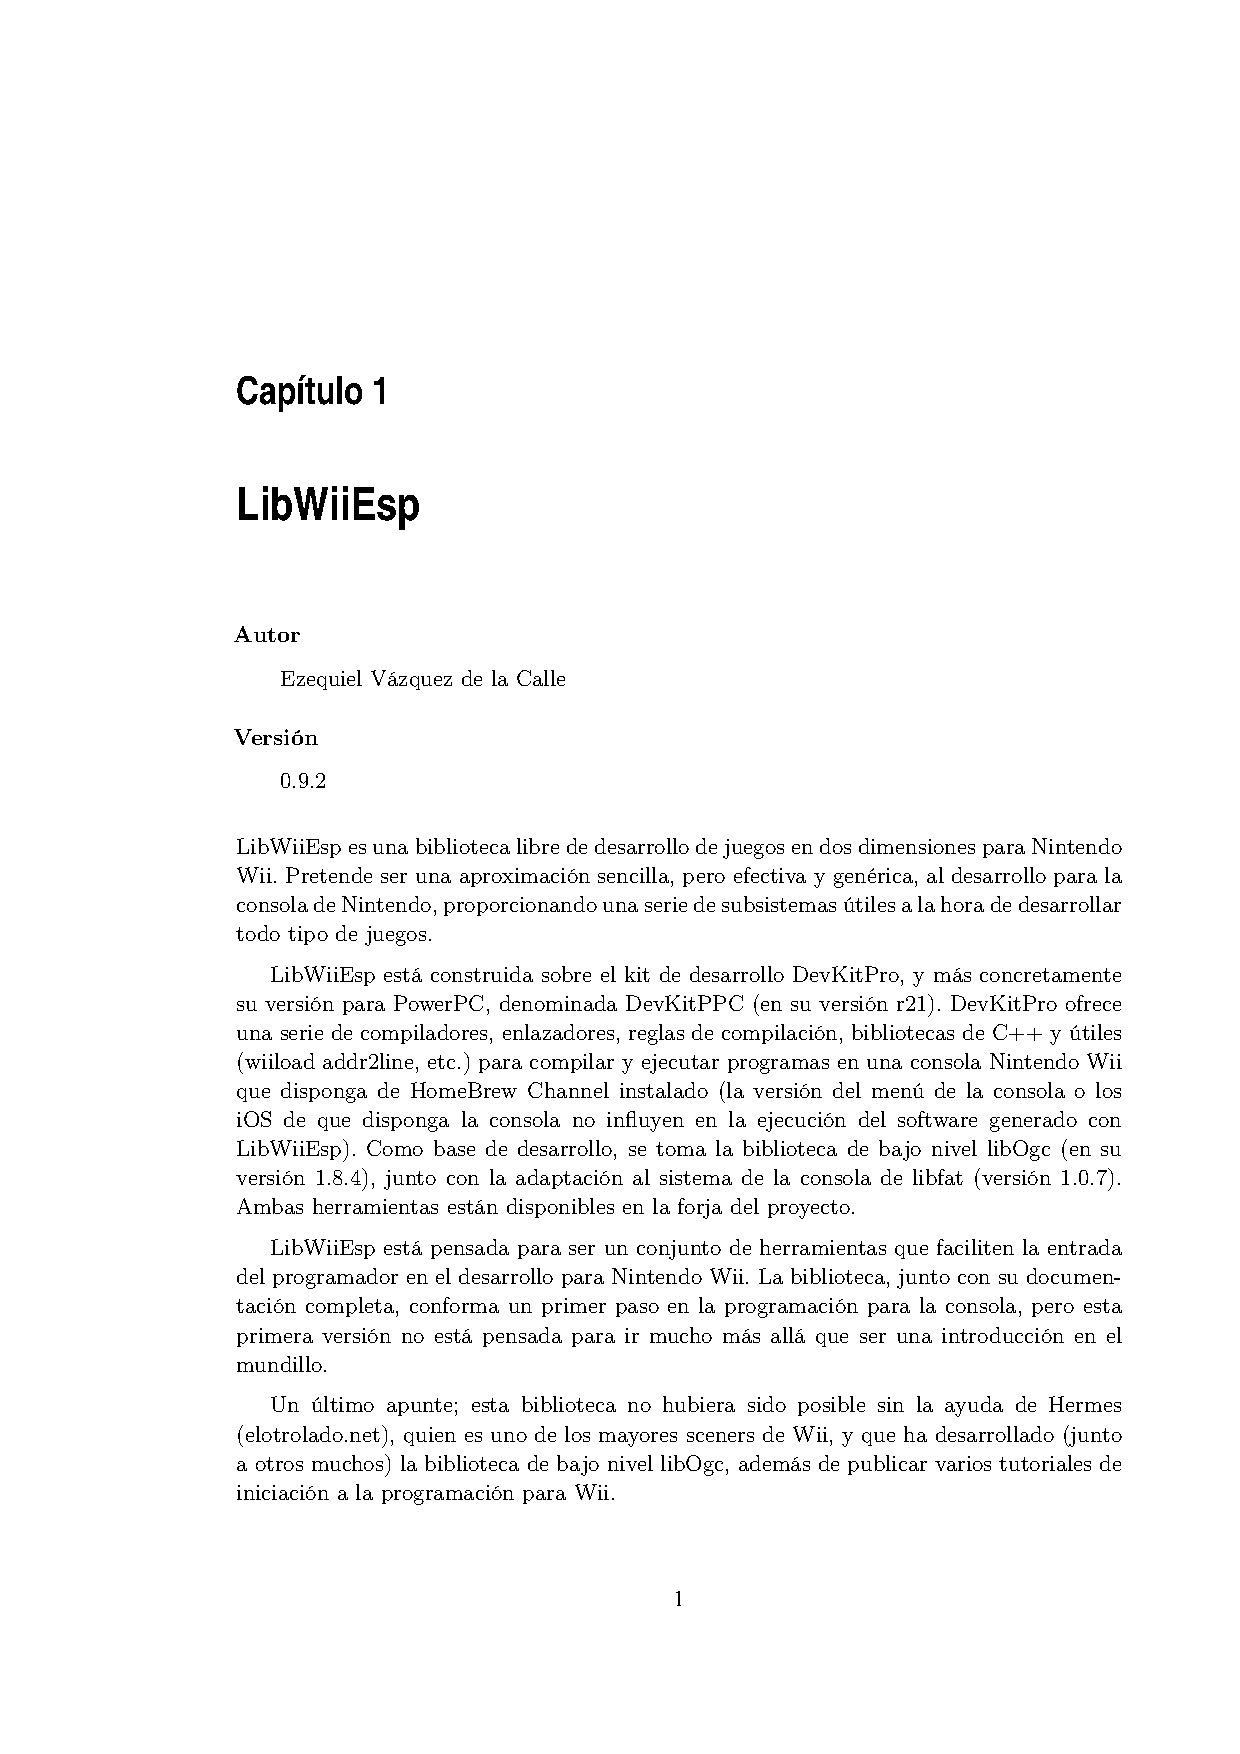
\includepdf[pages=-,pagecommand=\thispagestyle{fancy}]{./referencia/refman}


\input{fdl-1.3}

\end{document}
